\section[Factoring Out Symmetries in Concentration Profiles]{Factoring Out Symmetries in Concentration Profiles}

\begin{frame}{Importance of Symmetries in Data Analysis}

	\centering
	In the previous analysis, we first needed to determine \\where to open and ``unroll'' the circle
	
	\centering
	\begin{tikzpicture}
		\node (drosophila_line) {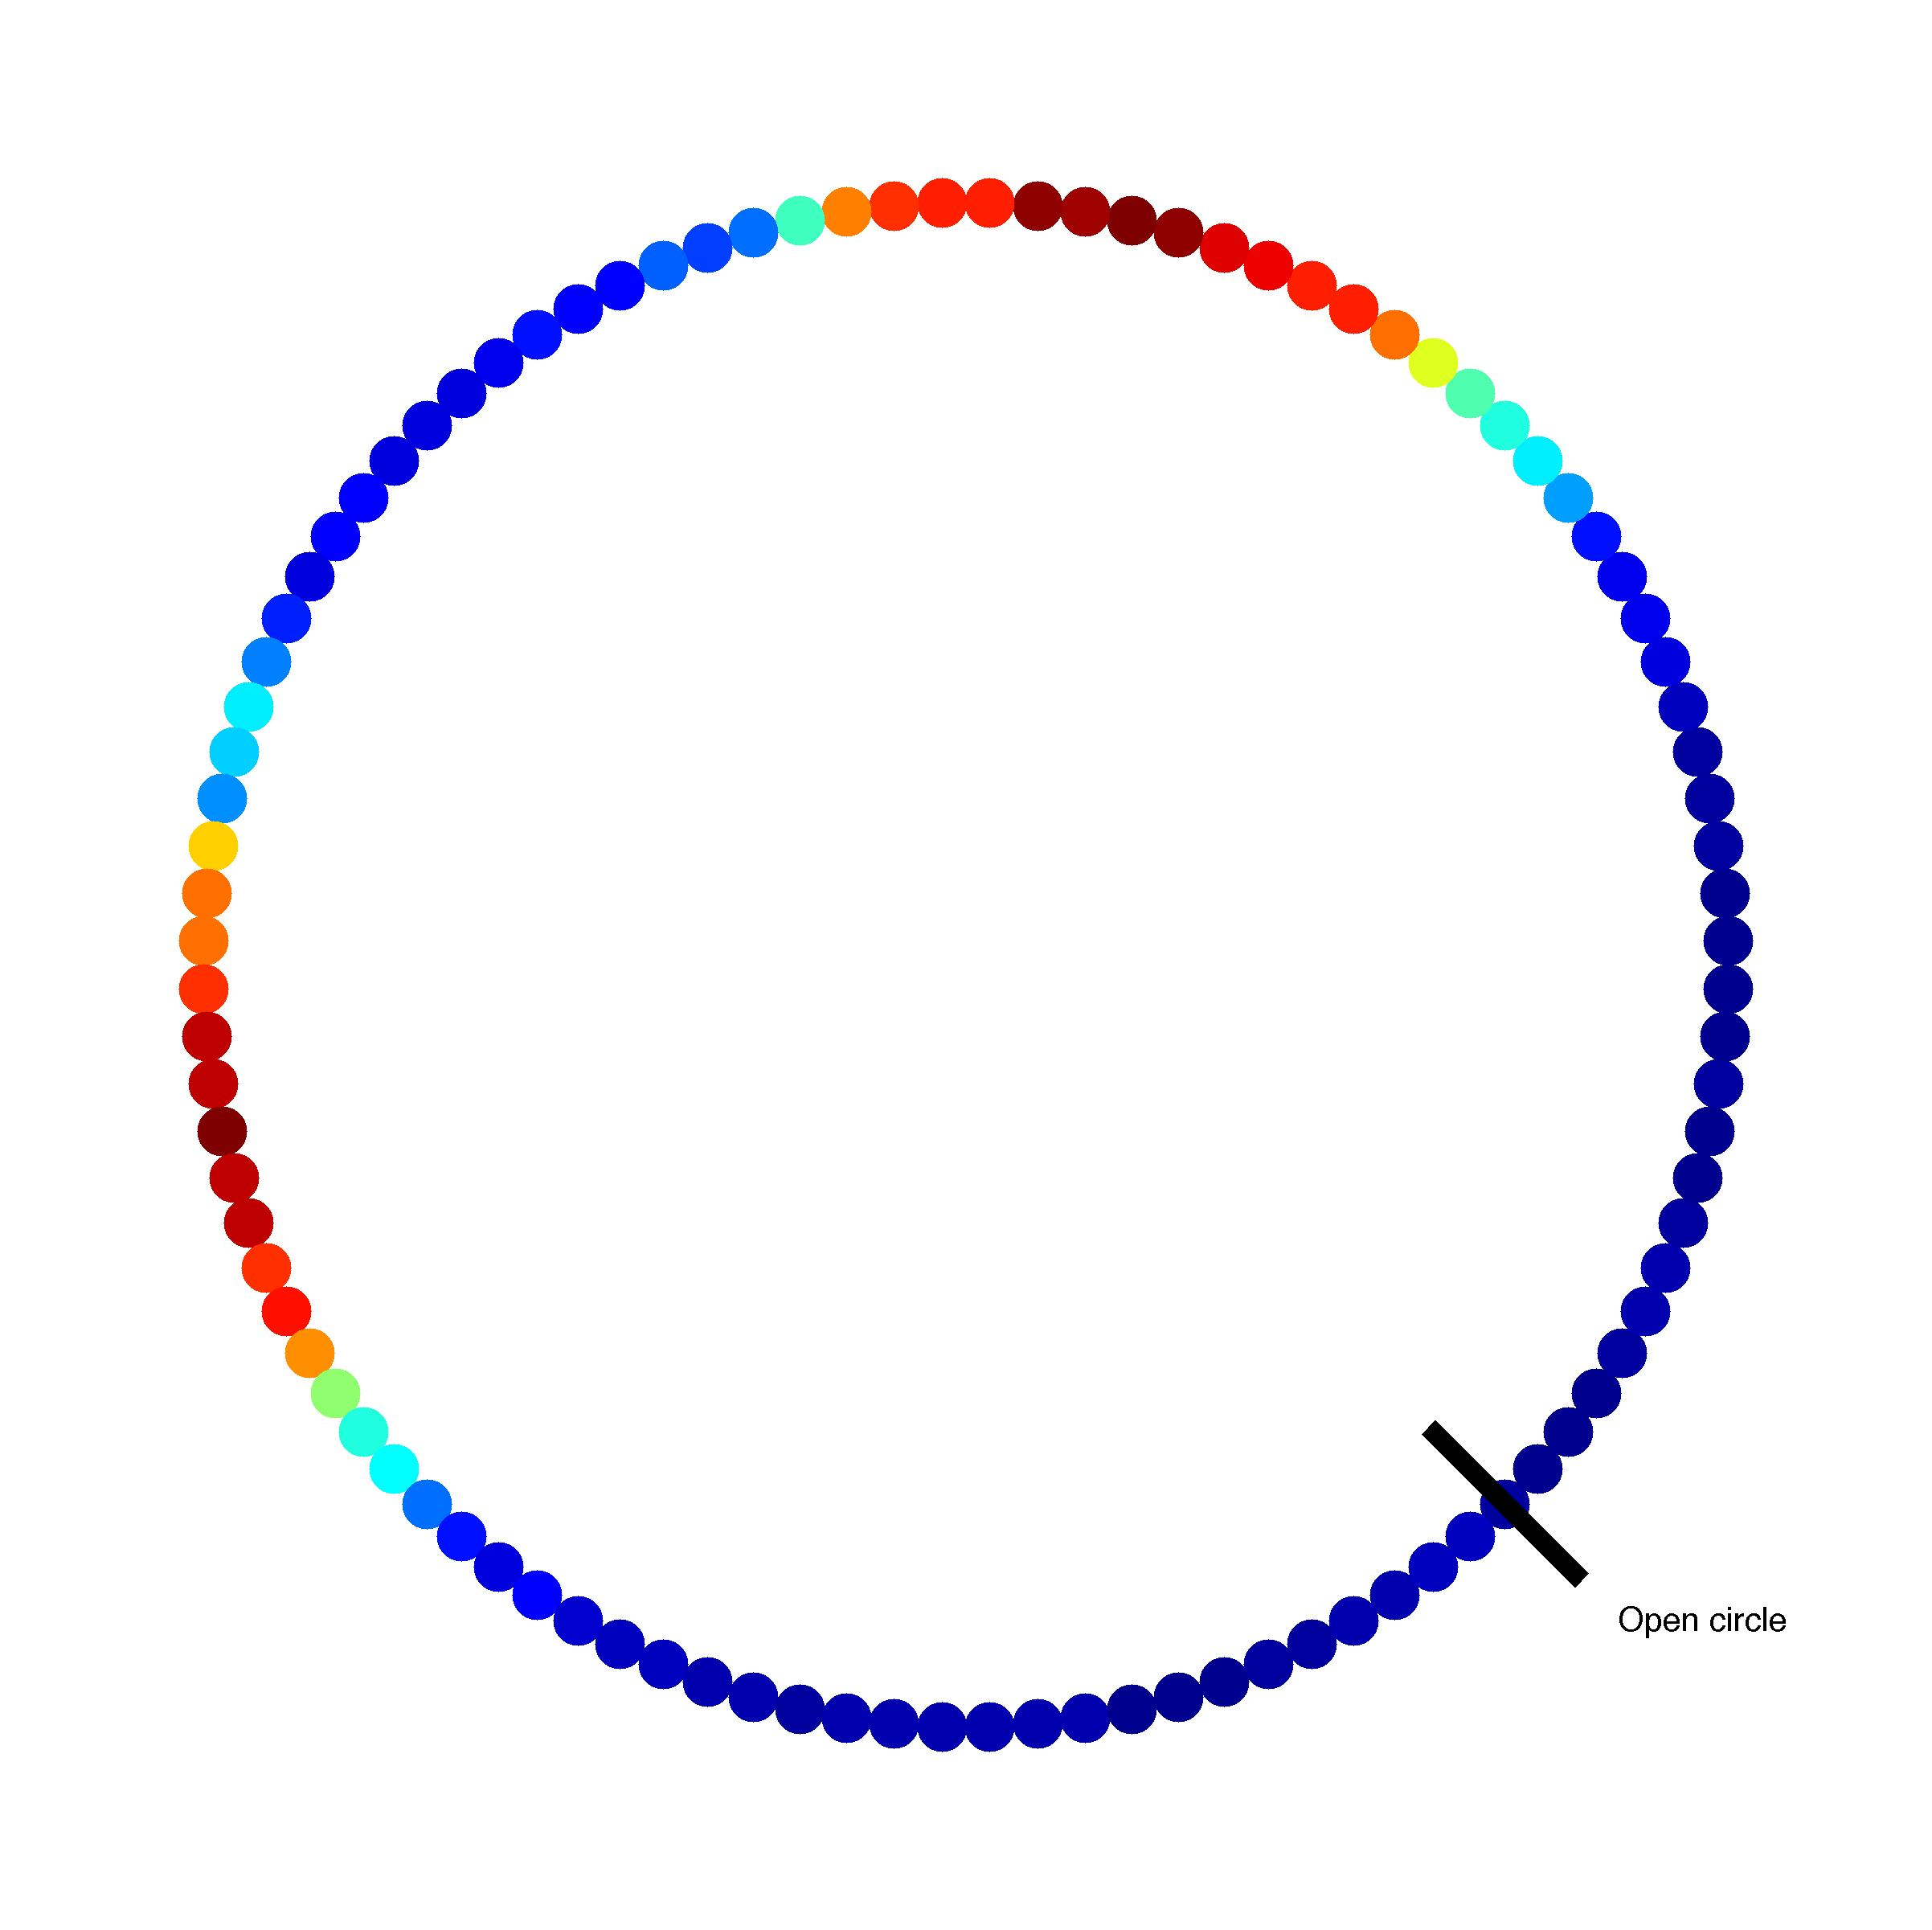
\includegraphics[width=0.2\textwidth]{circle_profile}};
		\node[right=0.3\textwidth of drosophila_line] (drosophila_circle) {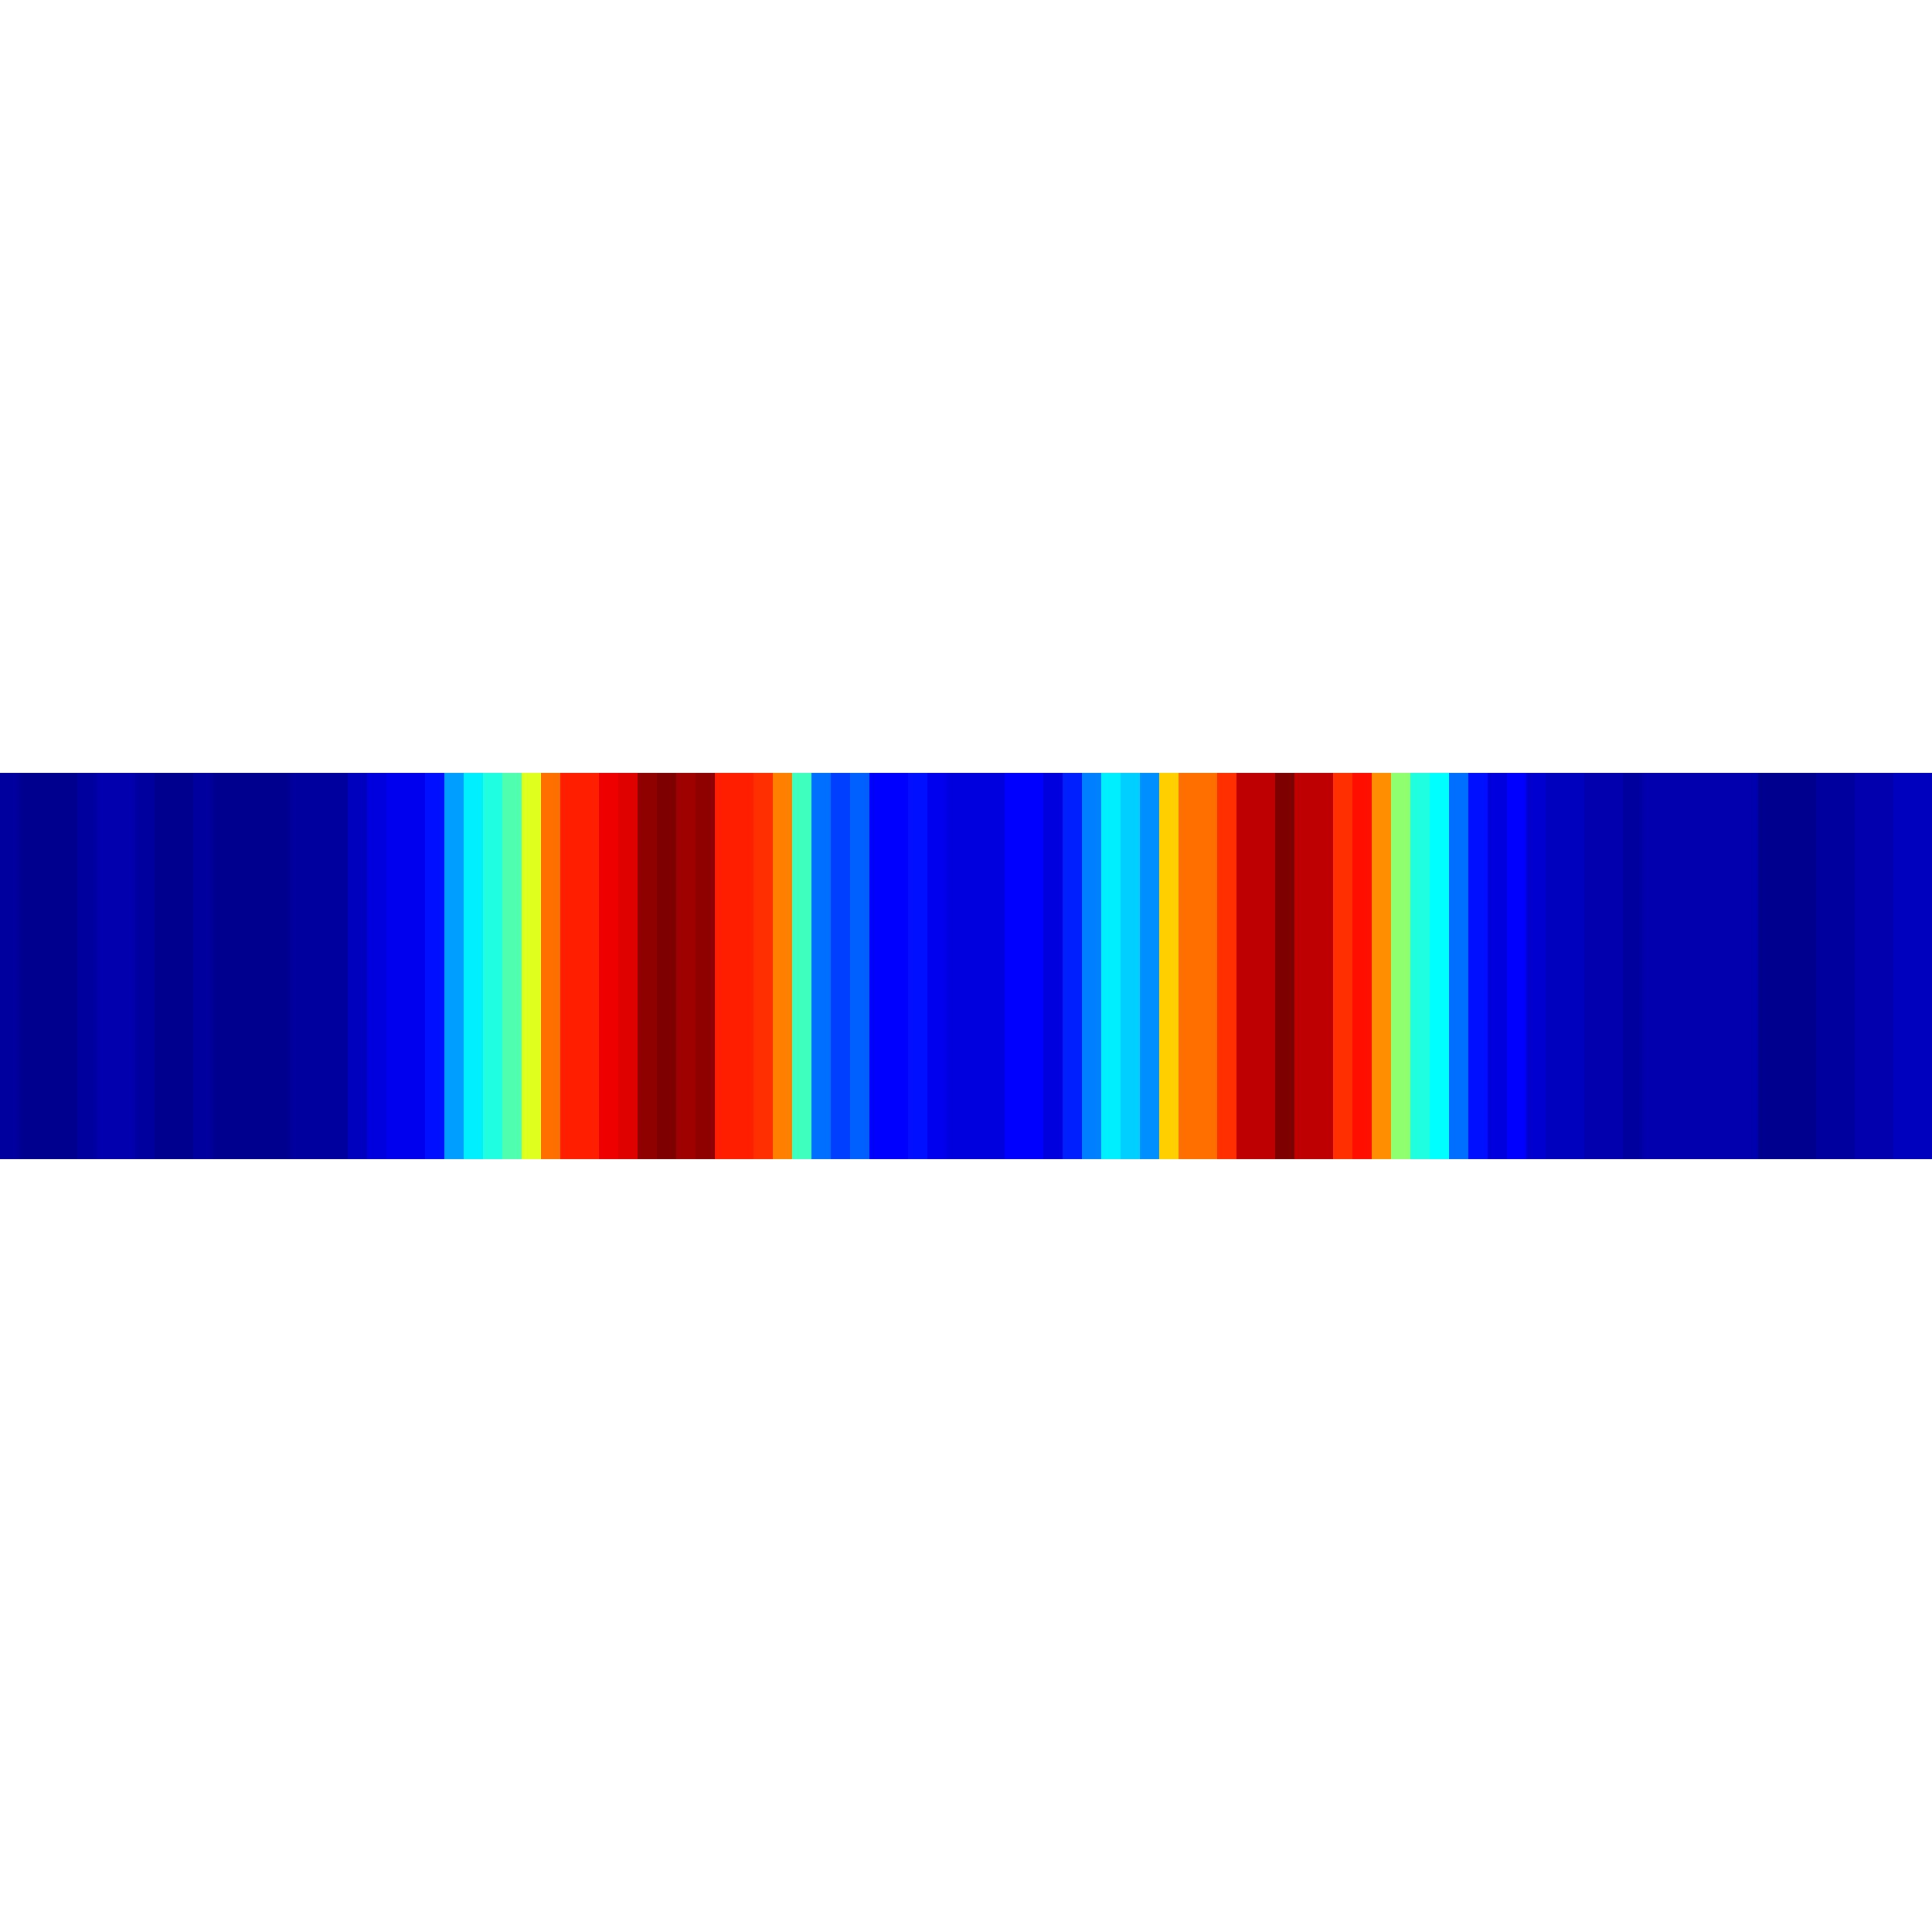
\includegraphics[width=0.25\textwidth, height=0.1in]{line_profile}};
		\draw[->] (drosophila_line) -- (drosophila_circle) node[above,midway] {``Unroll'' circle};
	\end{tikzpicture}
	
	This is done by staining for {\em another} protein (Dorsal) that is expressed only along the ventral midline, and then aligning the profiles along their ventral midlines.
	
	\vspace{0.2in}
	We would like to {\em automatically} align these concentration profiles\\
	without having to stain for a second protein.

\end{frame}

\begin{frame}{How to Address Rotation Invariance in Data Analysis}
    There are two ways to view rotation-invariant data
 
 	\begin{block}{}
        \begin{tikzpicture}
        	\node[text width=0.3\textwidth] (text1) {{\bf We can use rotations to {\em augment} data} \\ Given a data point $x$, we include all rotations of $x$ in our data set \par};
            \node[right=of text1] (fig1) {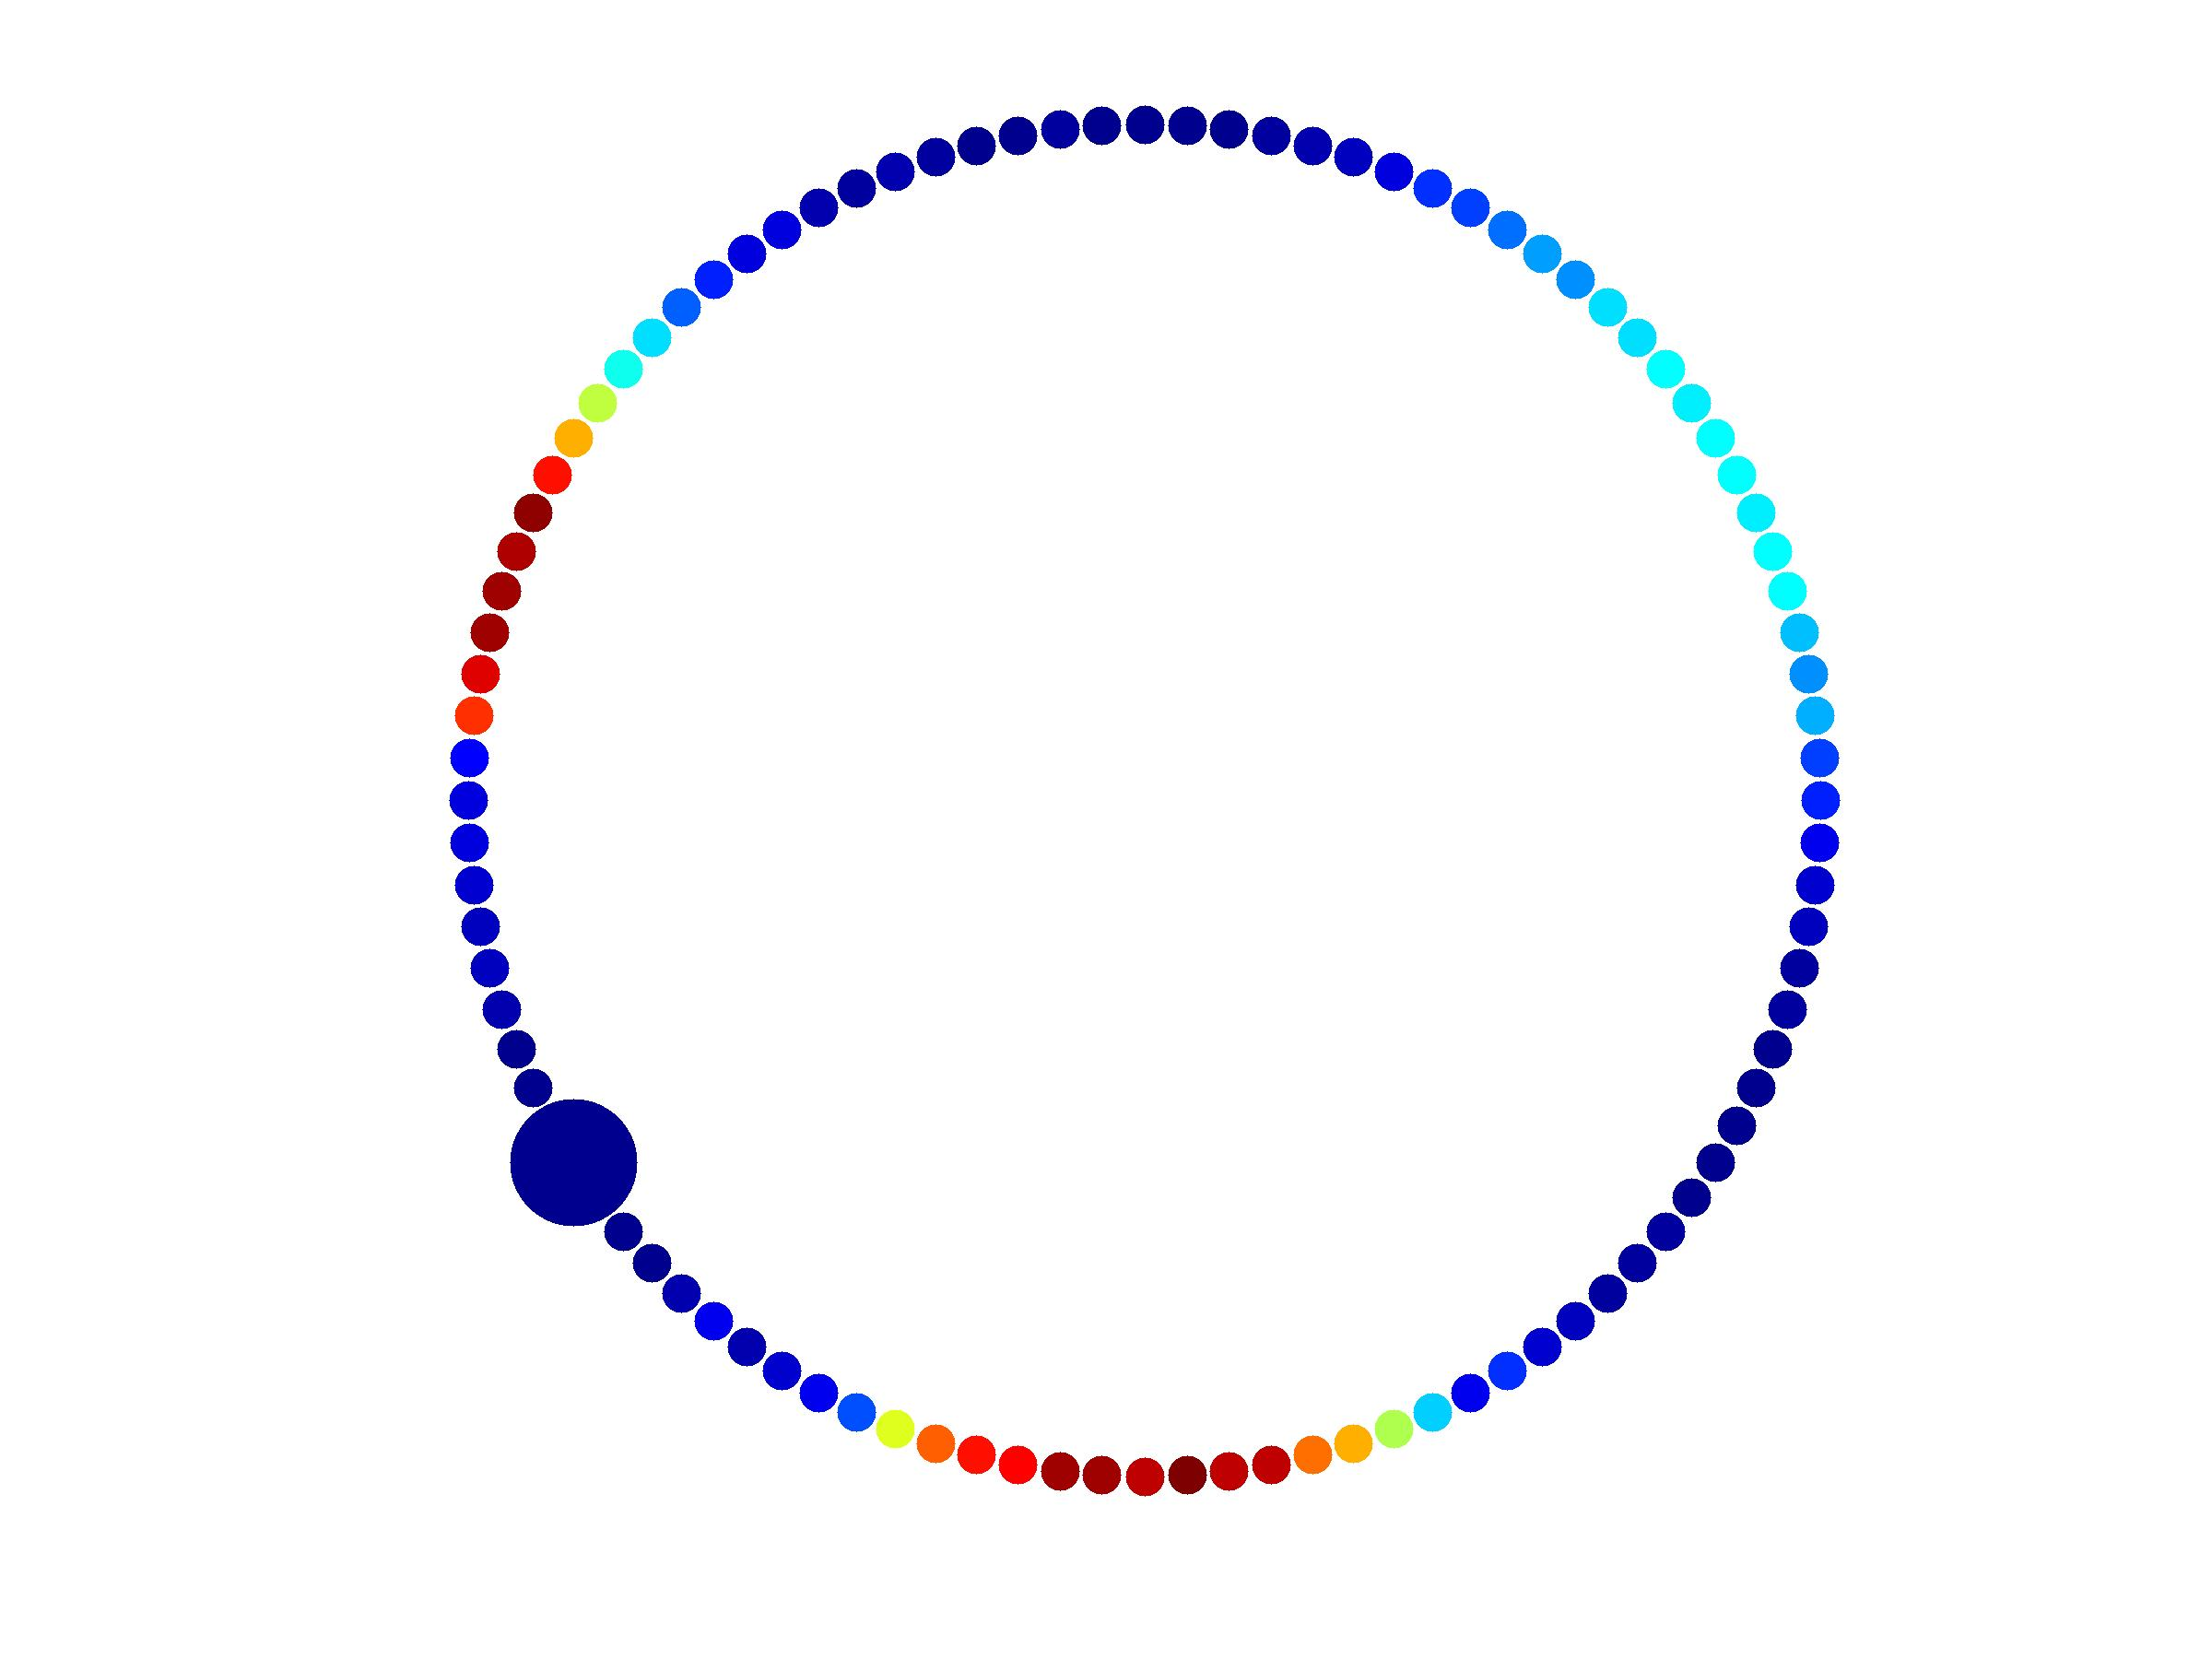
\includegraphics[width=0.25\textwidth]{../SIAM_DS_2013/drosophila_rot1.jpg}};
            \node [right of=fig1, node distance=0.35\textwidth] (fig2) {
            \begin{minipage}{0.25\textwidth}
                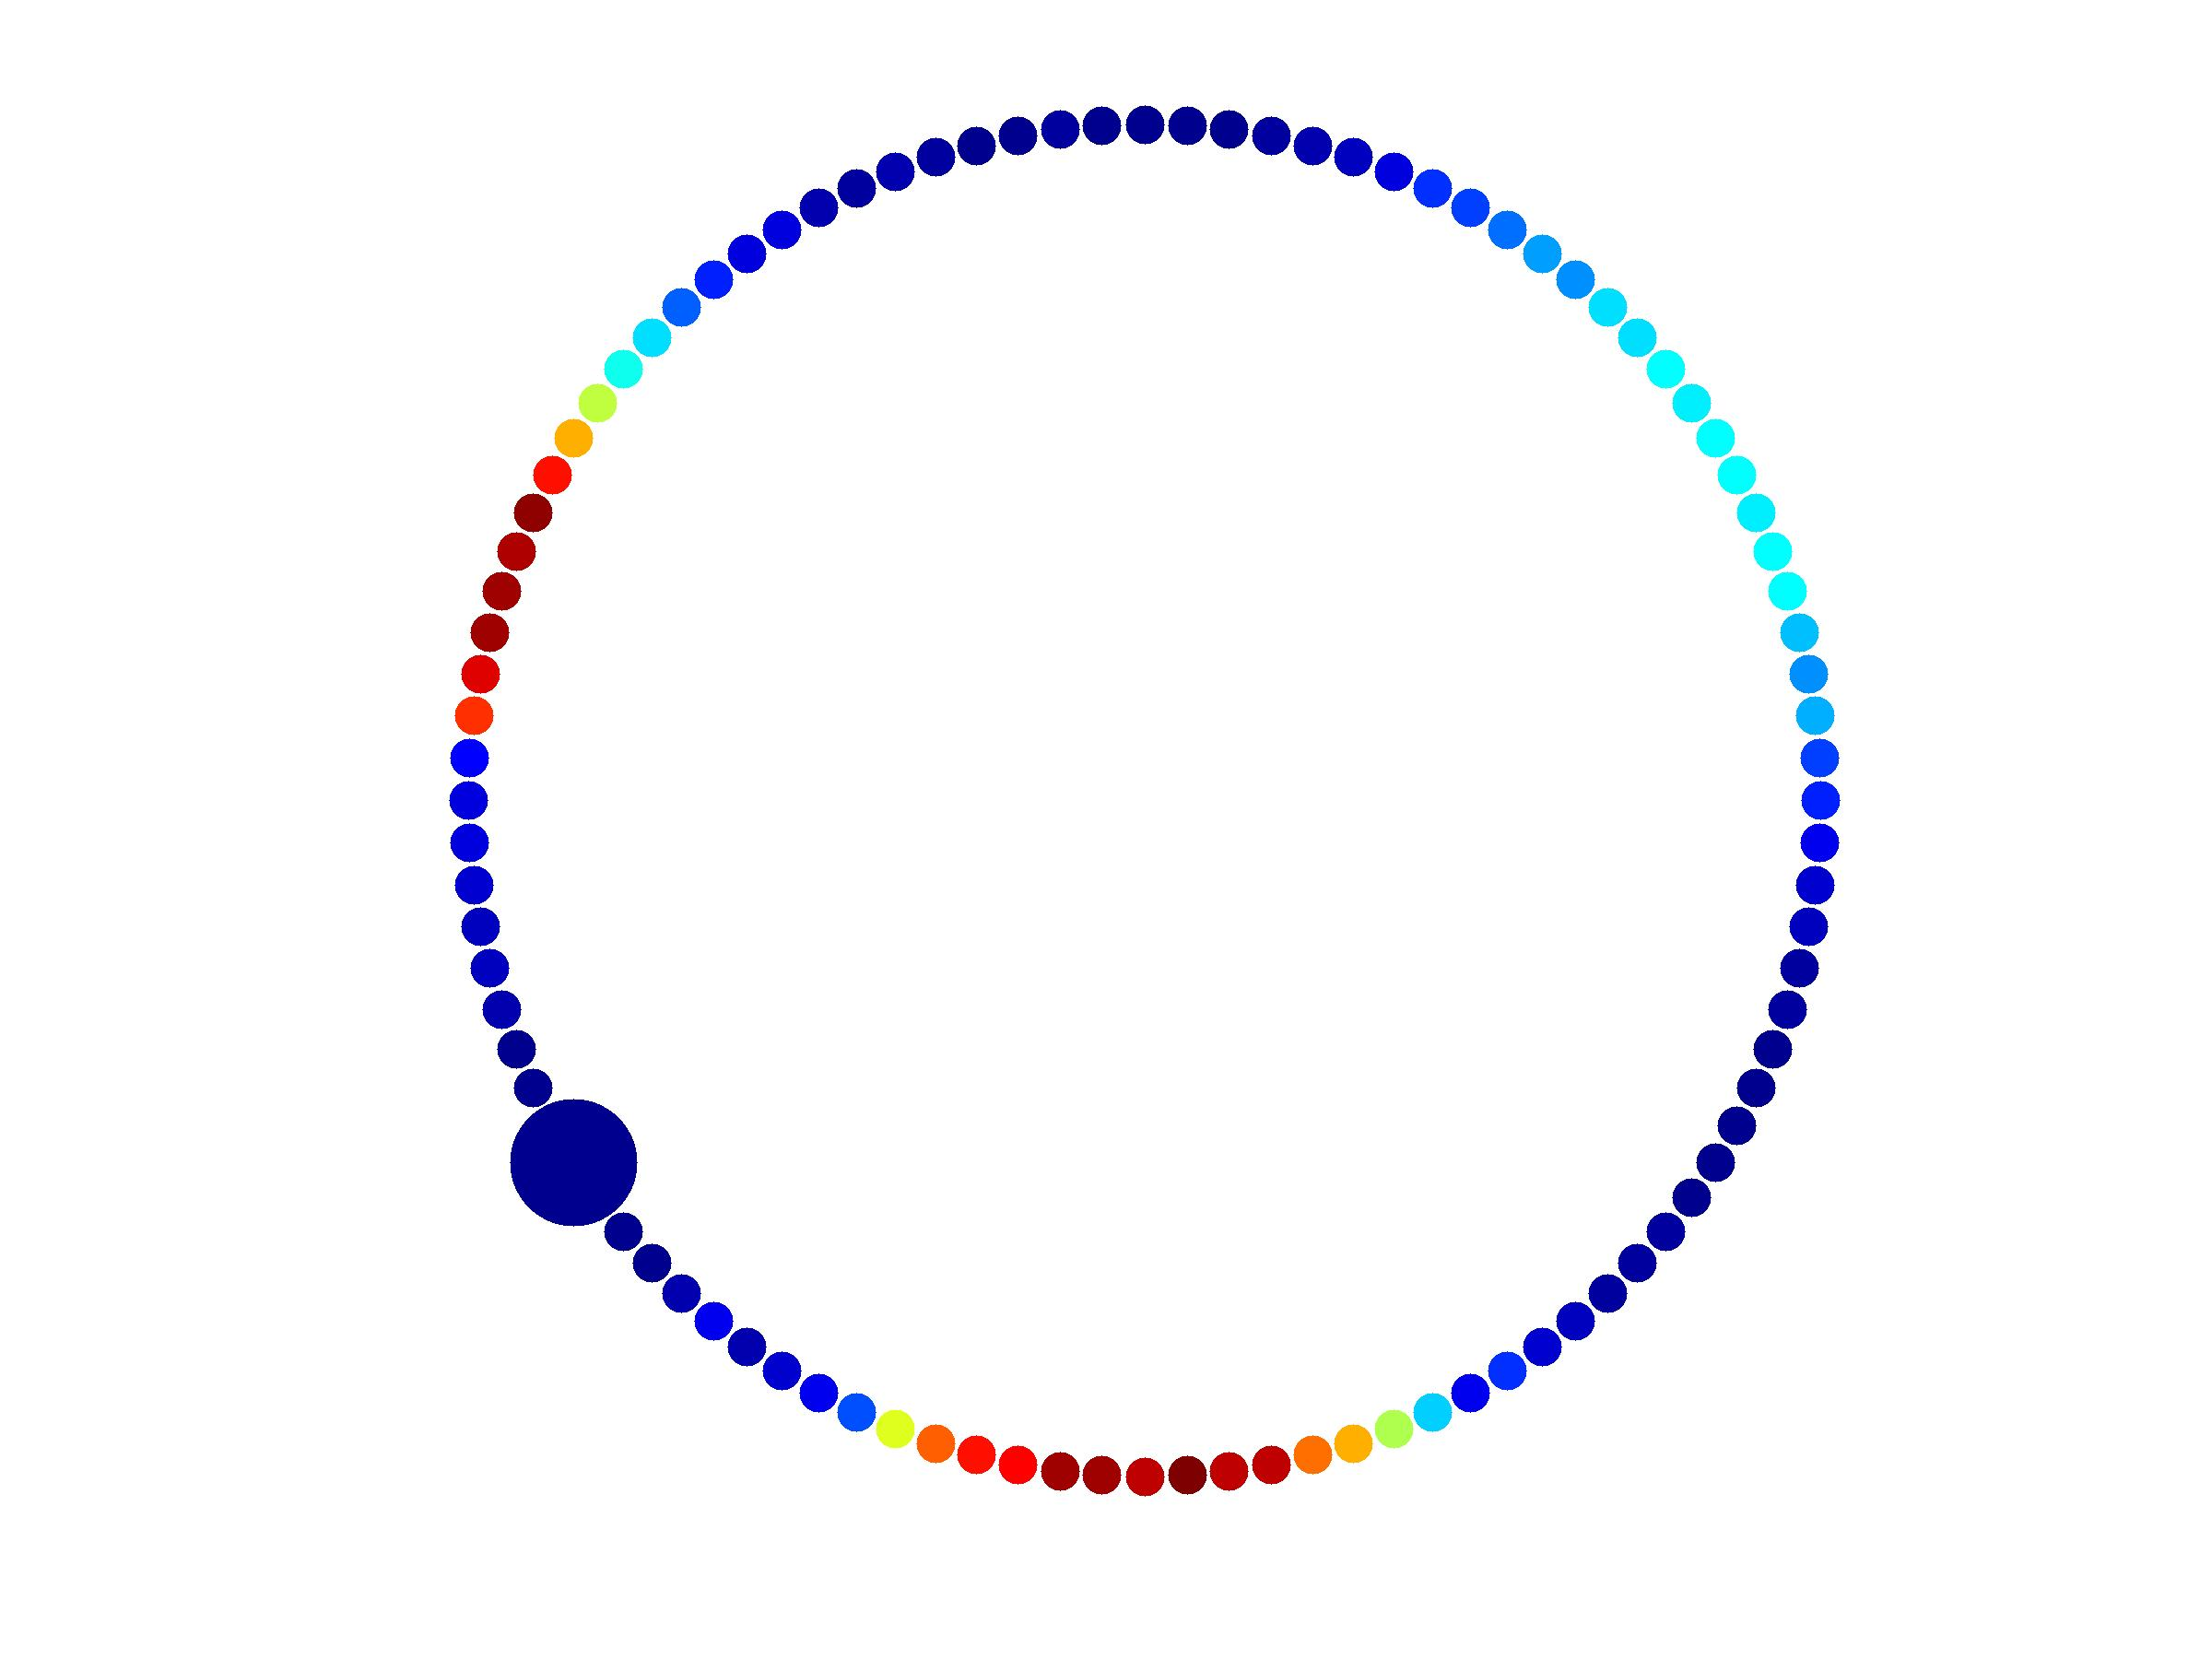
\includegraphics[width=0.45\textwidth]{../SIAM_DS_2013/drosophila_rot1.jpg}
                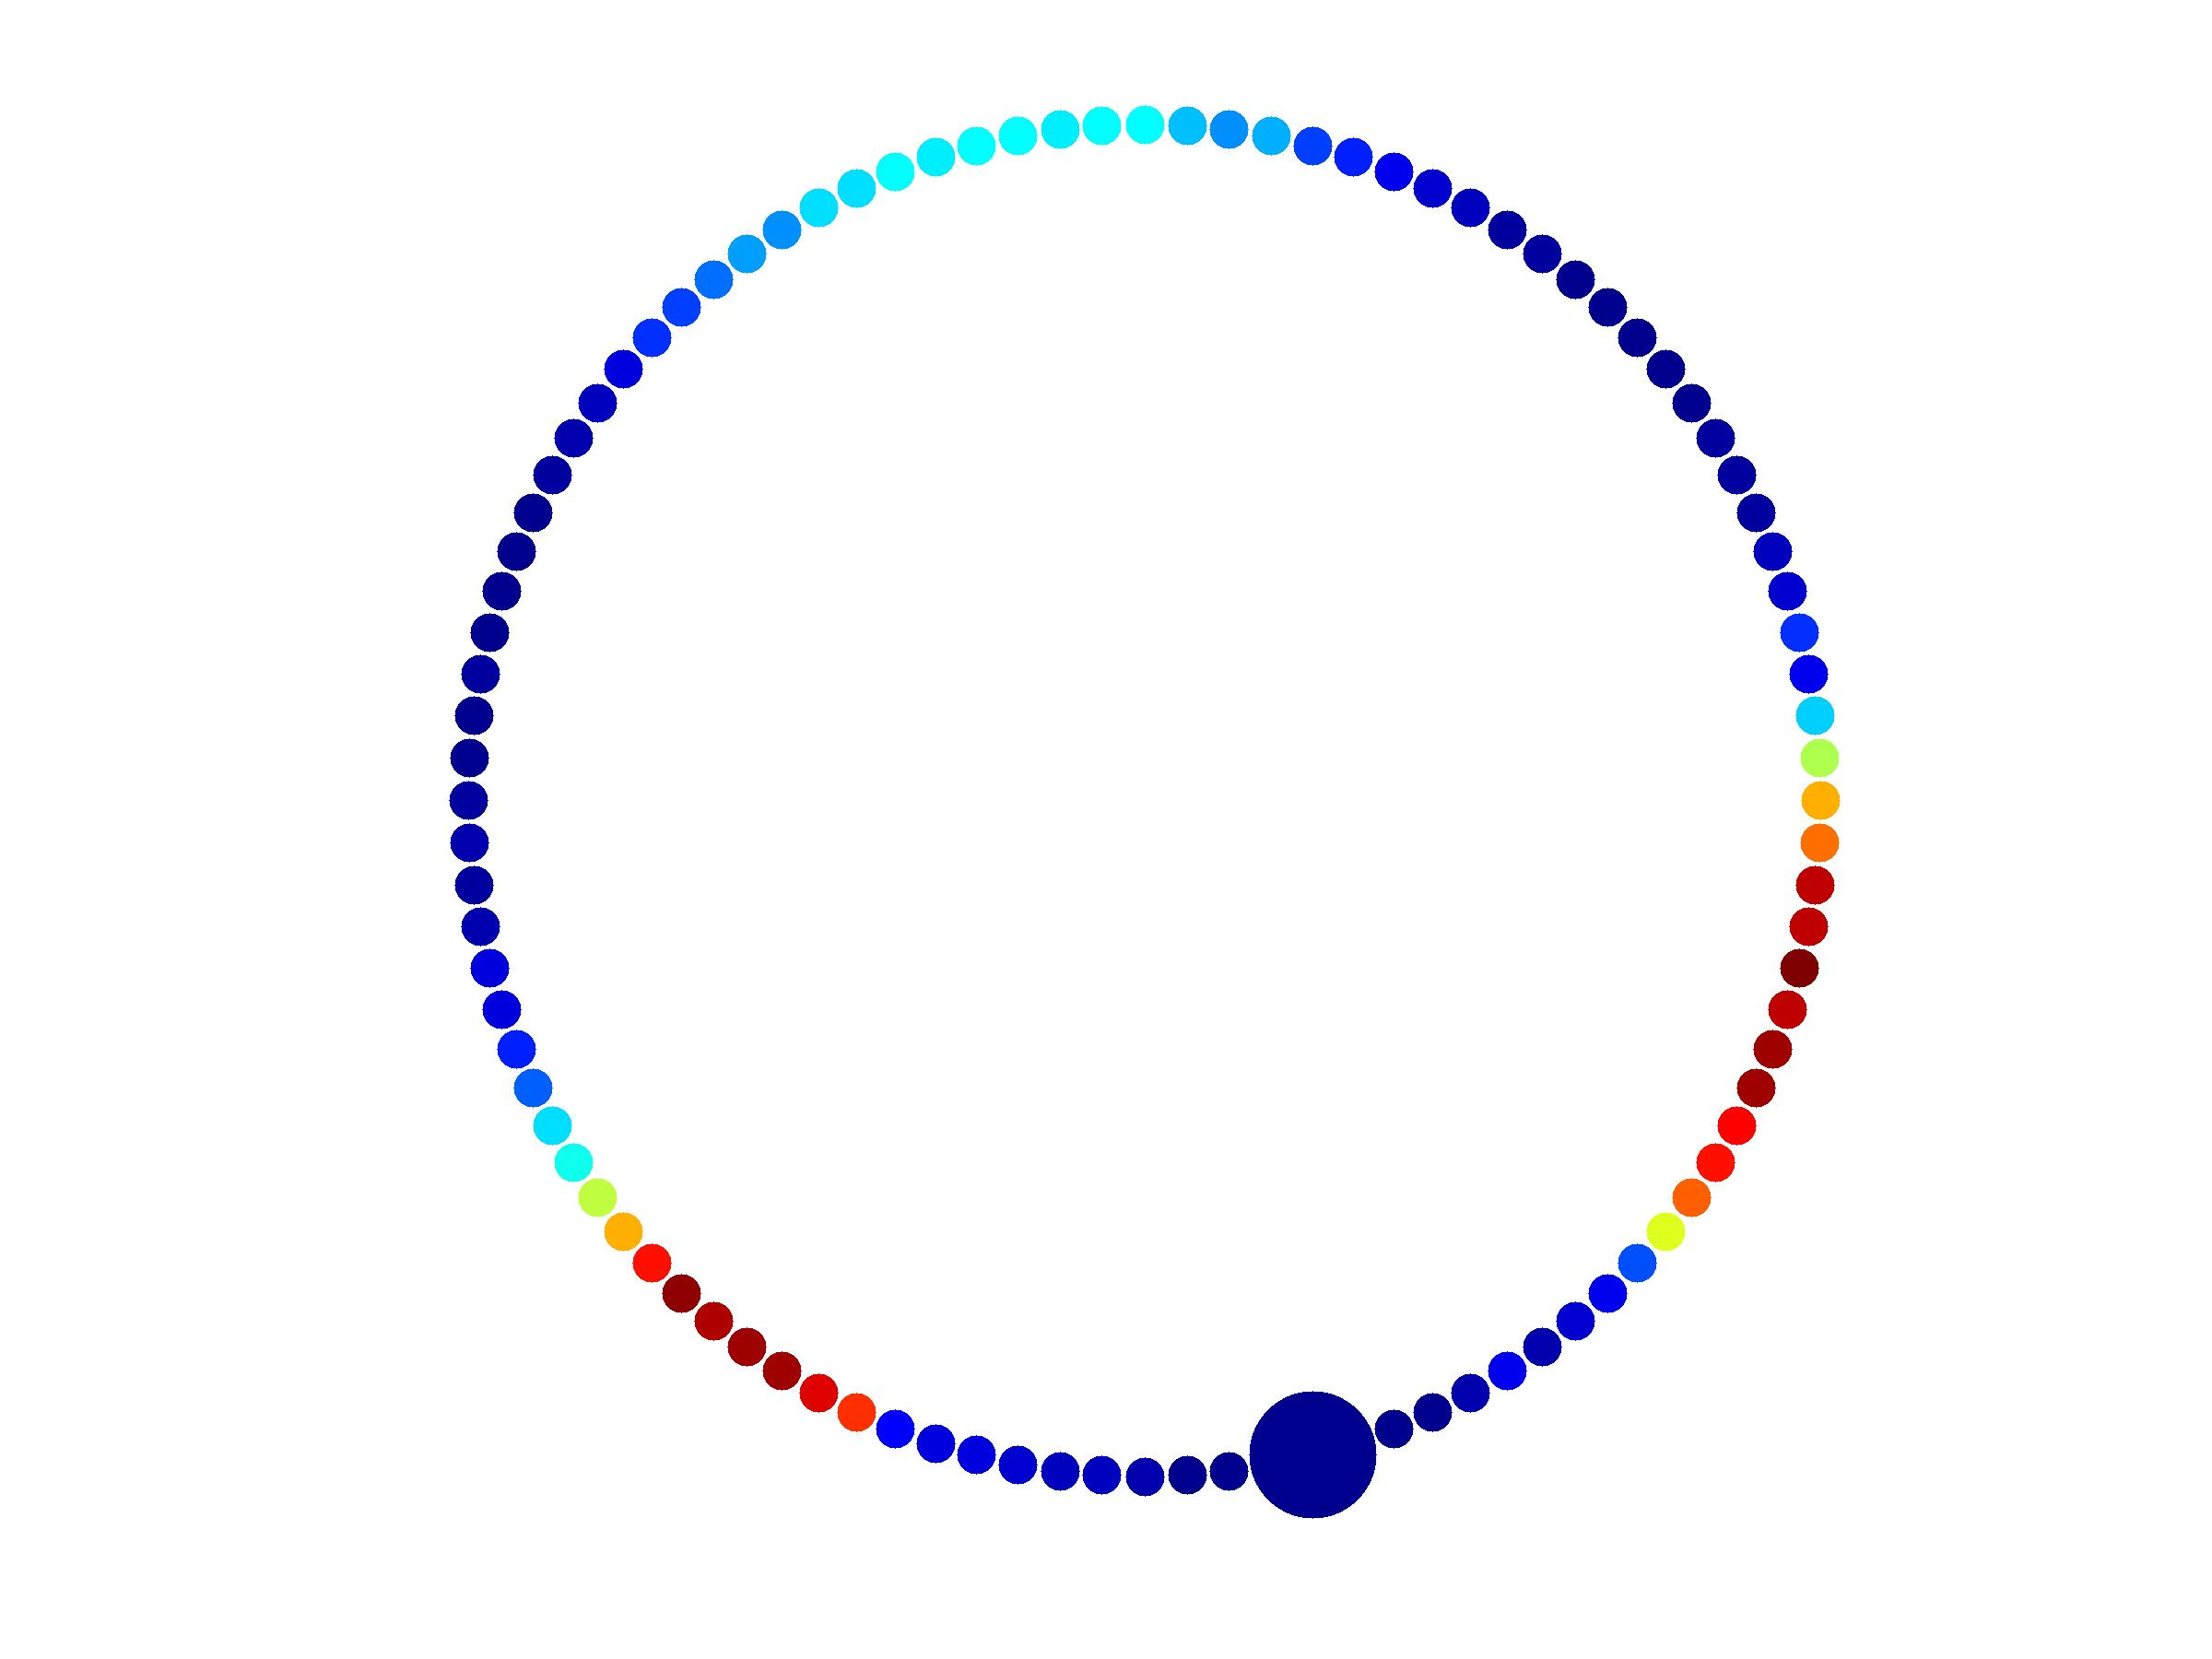
\includegraphics[width=0.45\textwidth]{../SIAM_DS_2013/drosophila_rot3.jpg}\\
                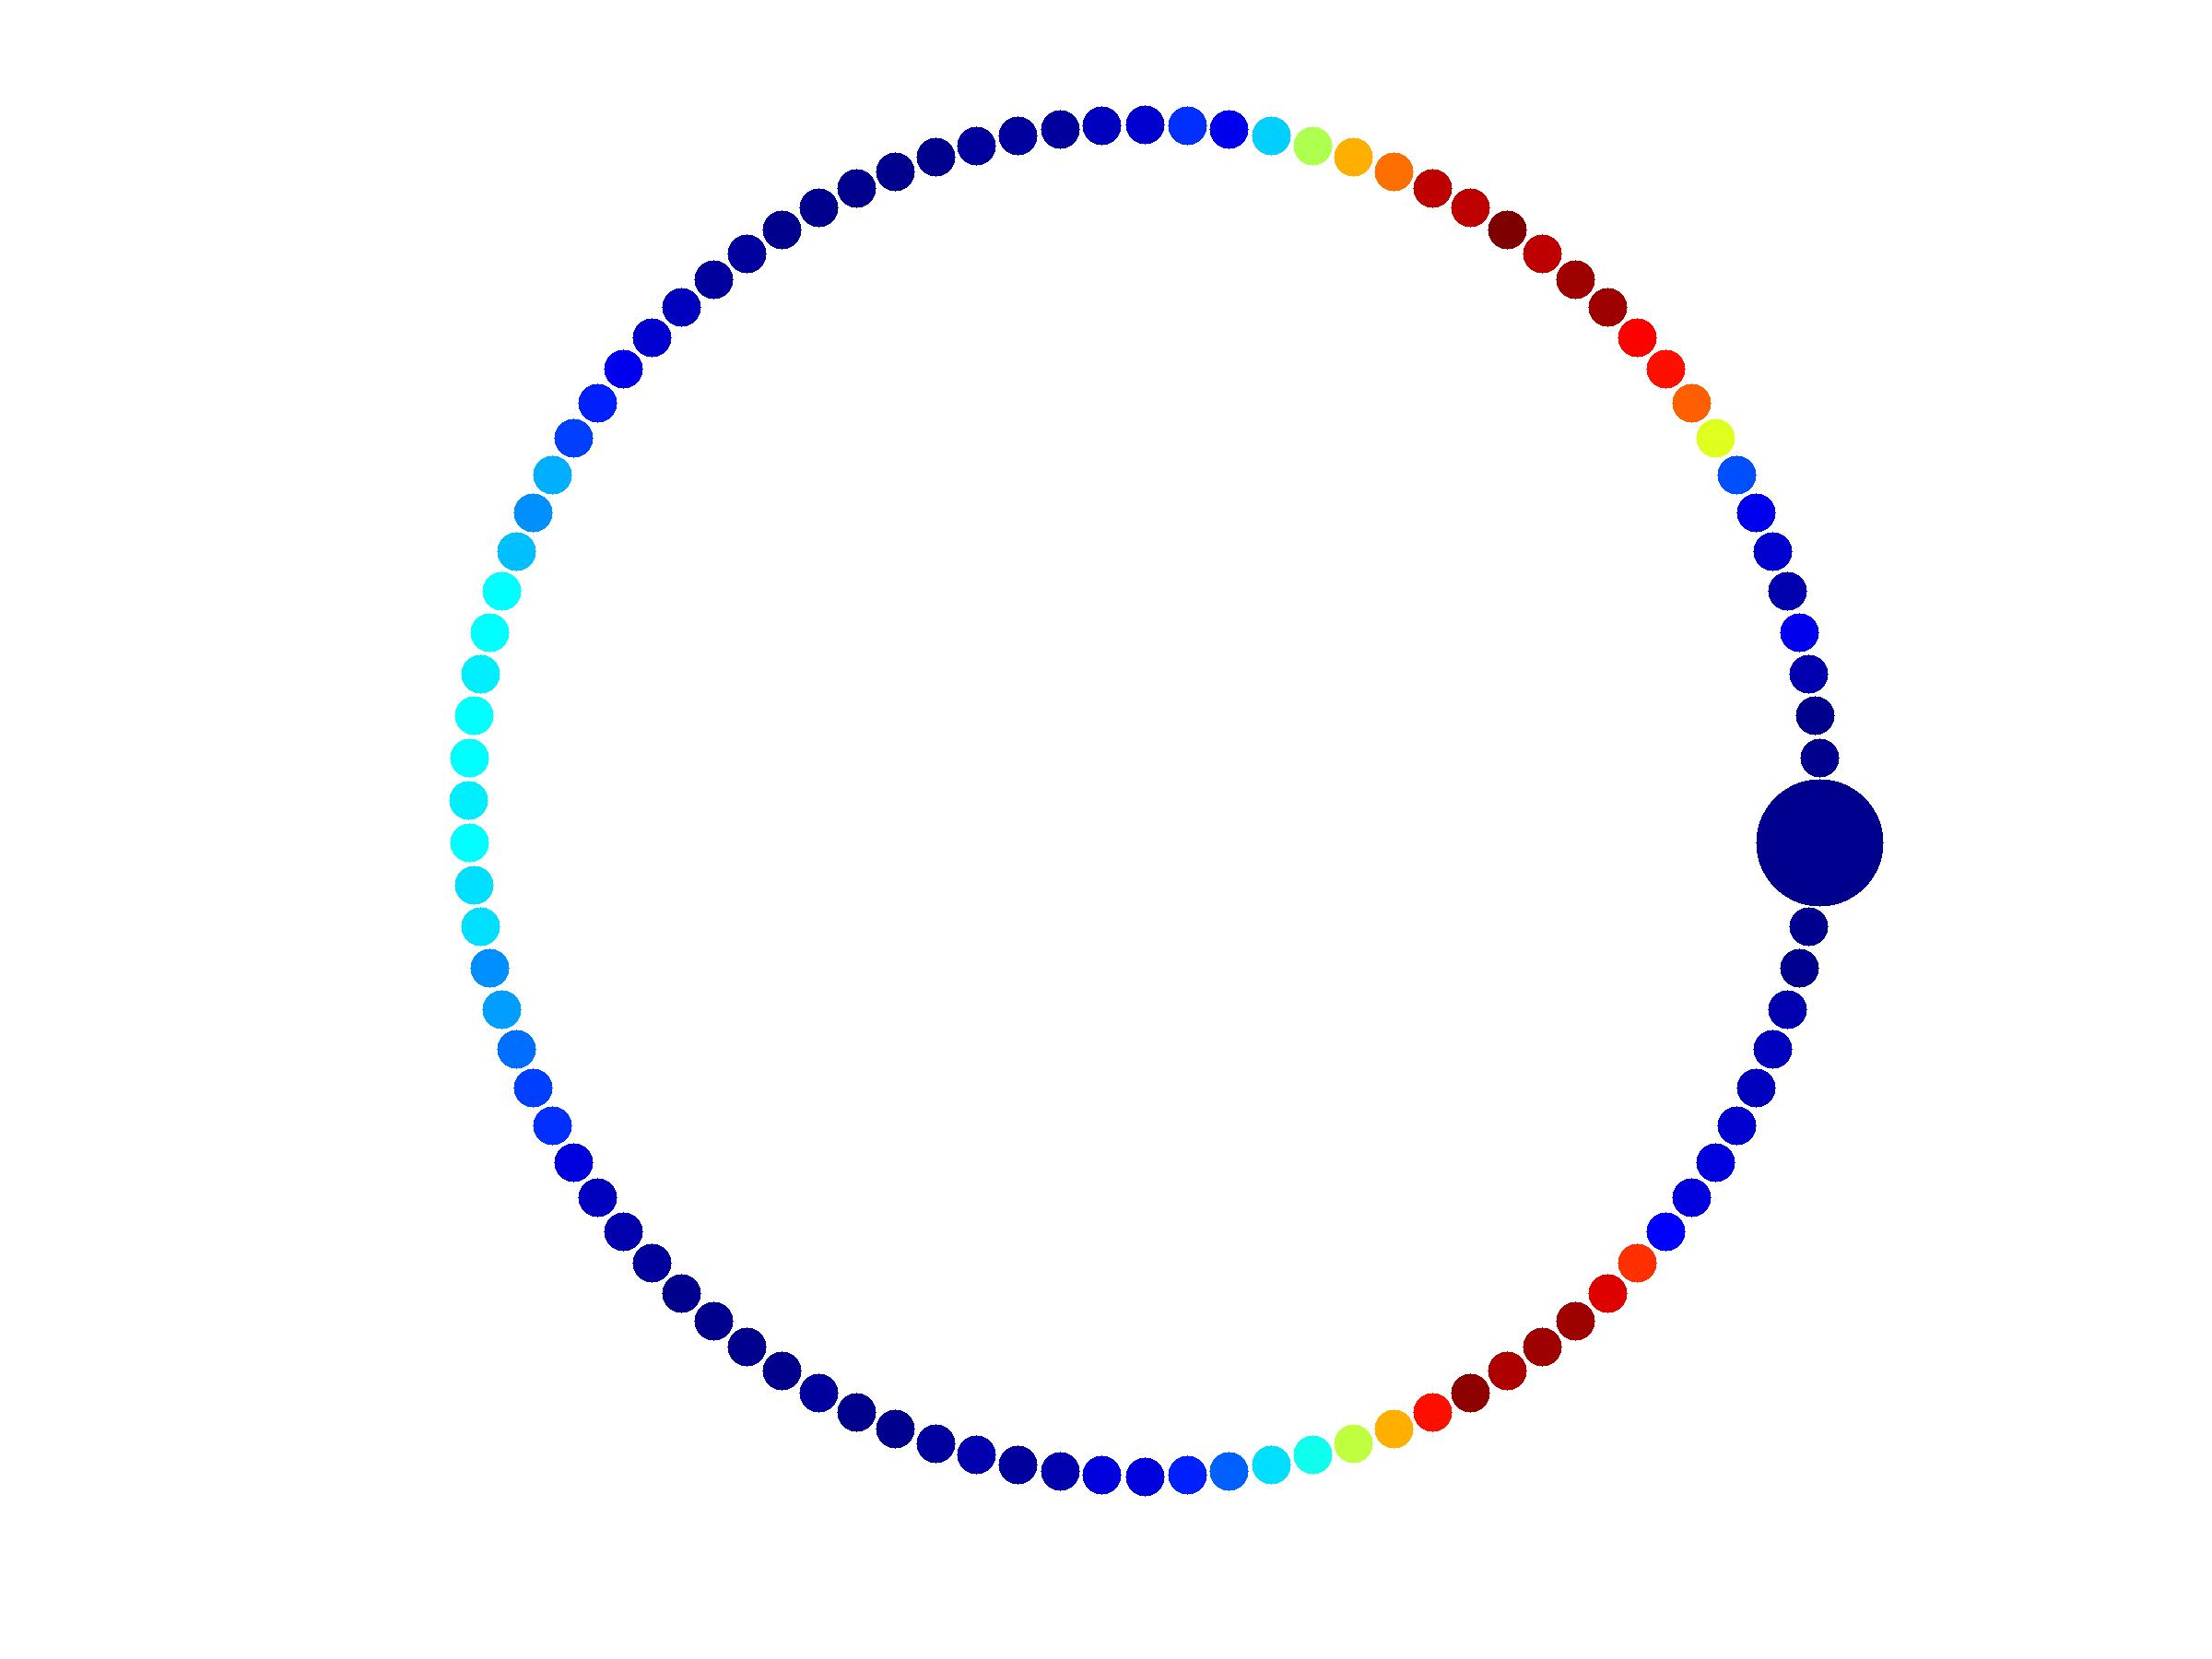
\includegraphics[width=0.45\textwidth]{../SIAM_DS_2013/drosophila_rot5.jpg}
                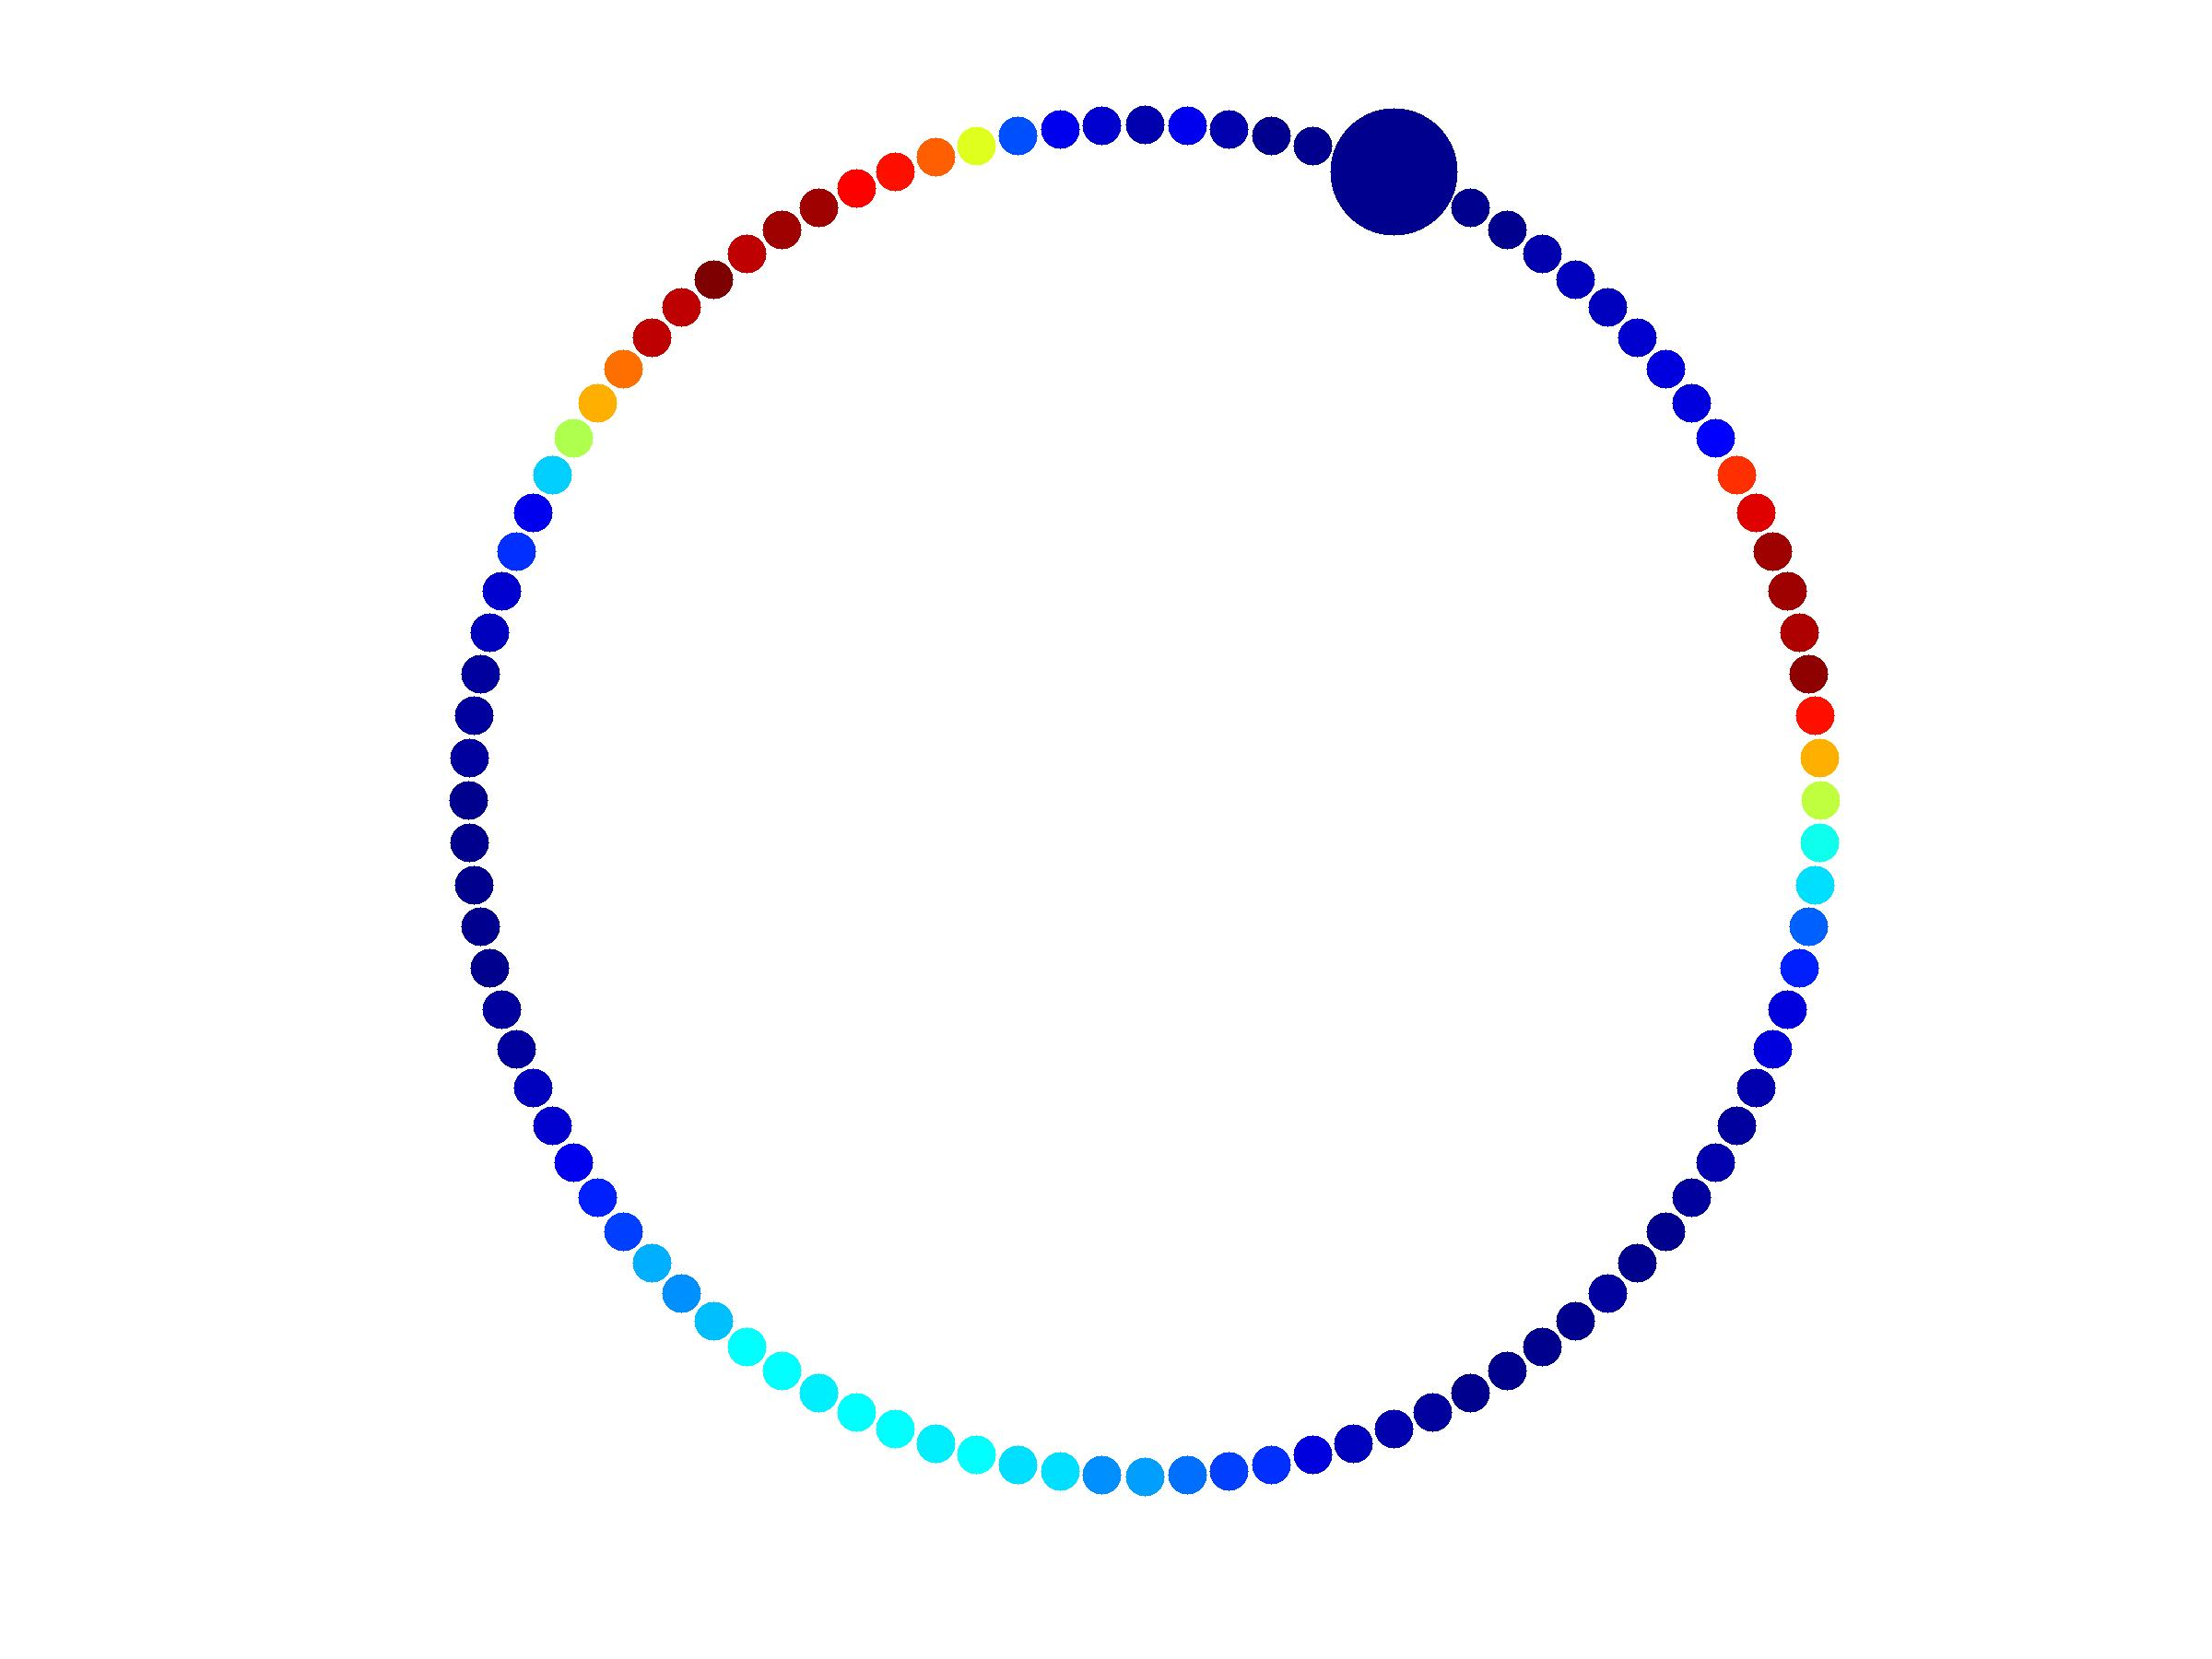
\includegraphics[width=0.45\textwidth]{../SIAM_DS_2013/drosophila_rot7.jpg}
            \end{minipage}};
            \draw [->] (fig1.east) -- (fig2.west);
        \end{tikzpicture}
        {\scriptsize \em This results in sines and cosines as PCA modes \footnotemark \par}
	\end{block}
	
	\footcitetext{sirovich1987turbulence}
	
	\vspace{-0.3in}
	
	\begin{block}{}
        \begin{tikzpicture}
        	\node [text width=0.3\textwidth] (text1) {{\bf We can use rotations to {\em reduce} data} \\ We first align the data before doing further analysis};
            \node[right=of text1] (fig1) {
            \begin{minipage}{0.25\textwidth}
            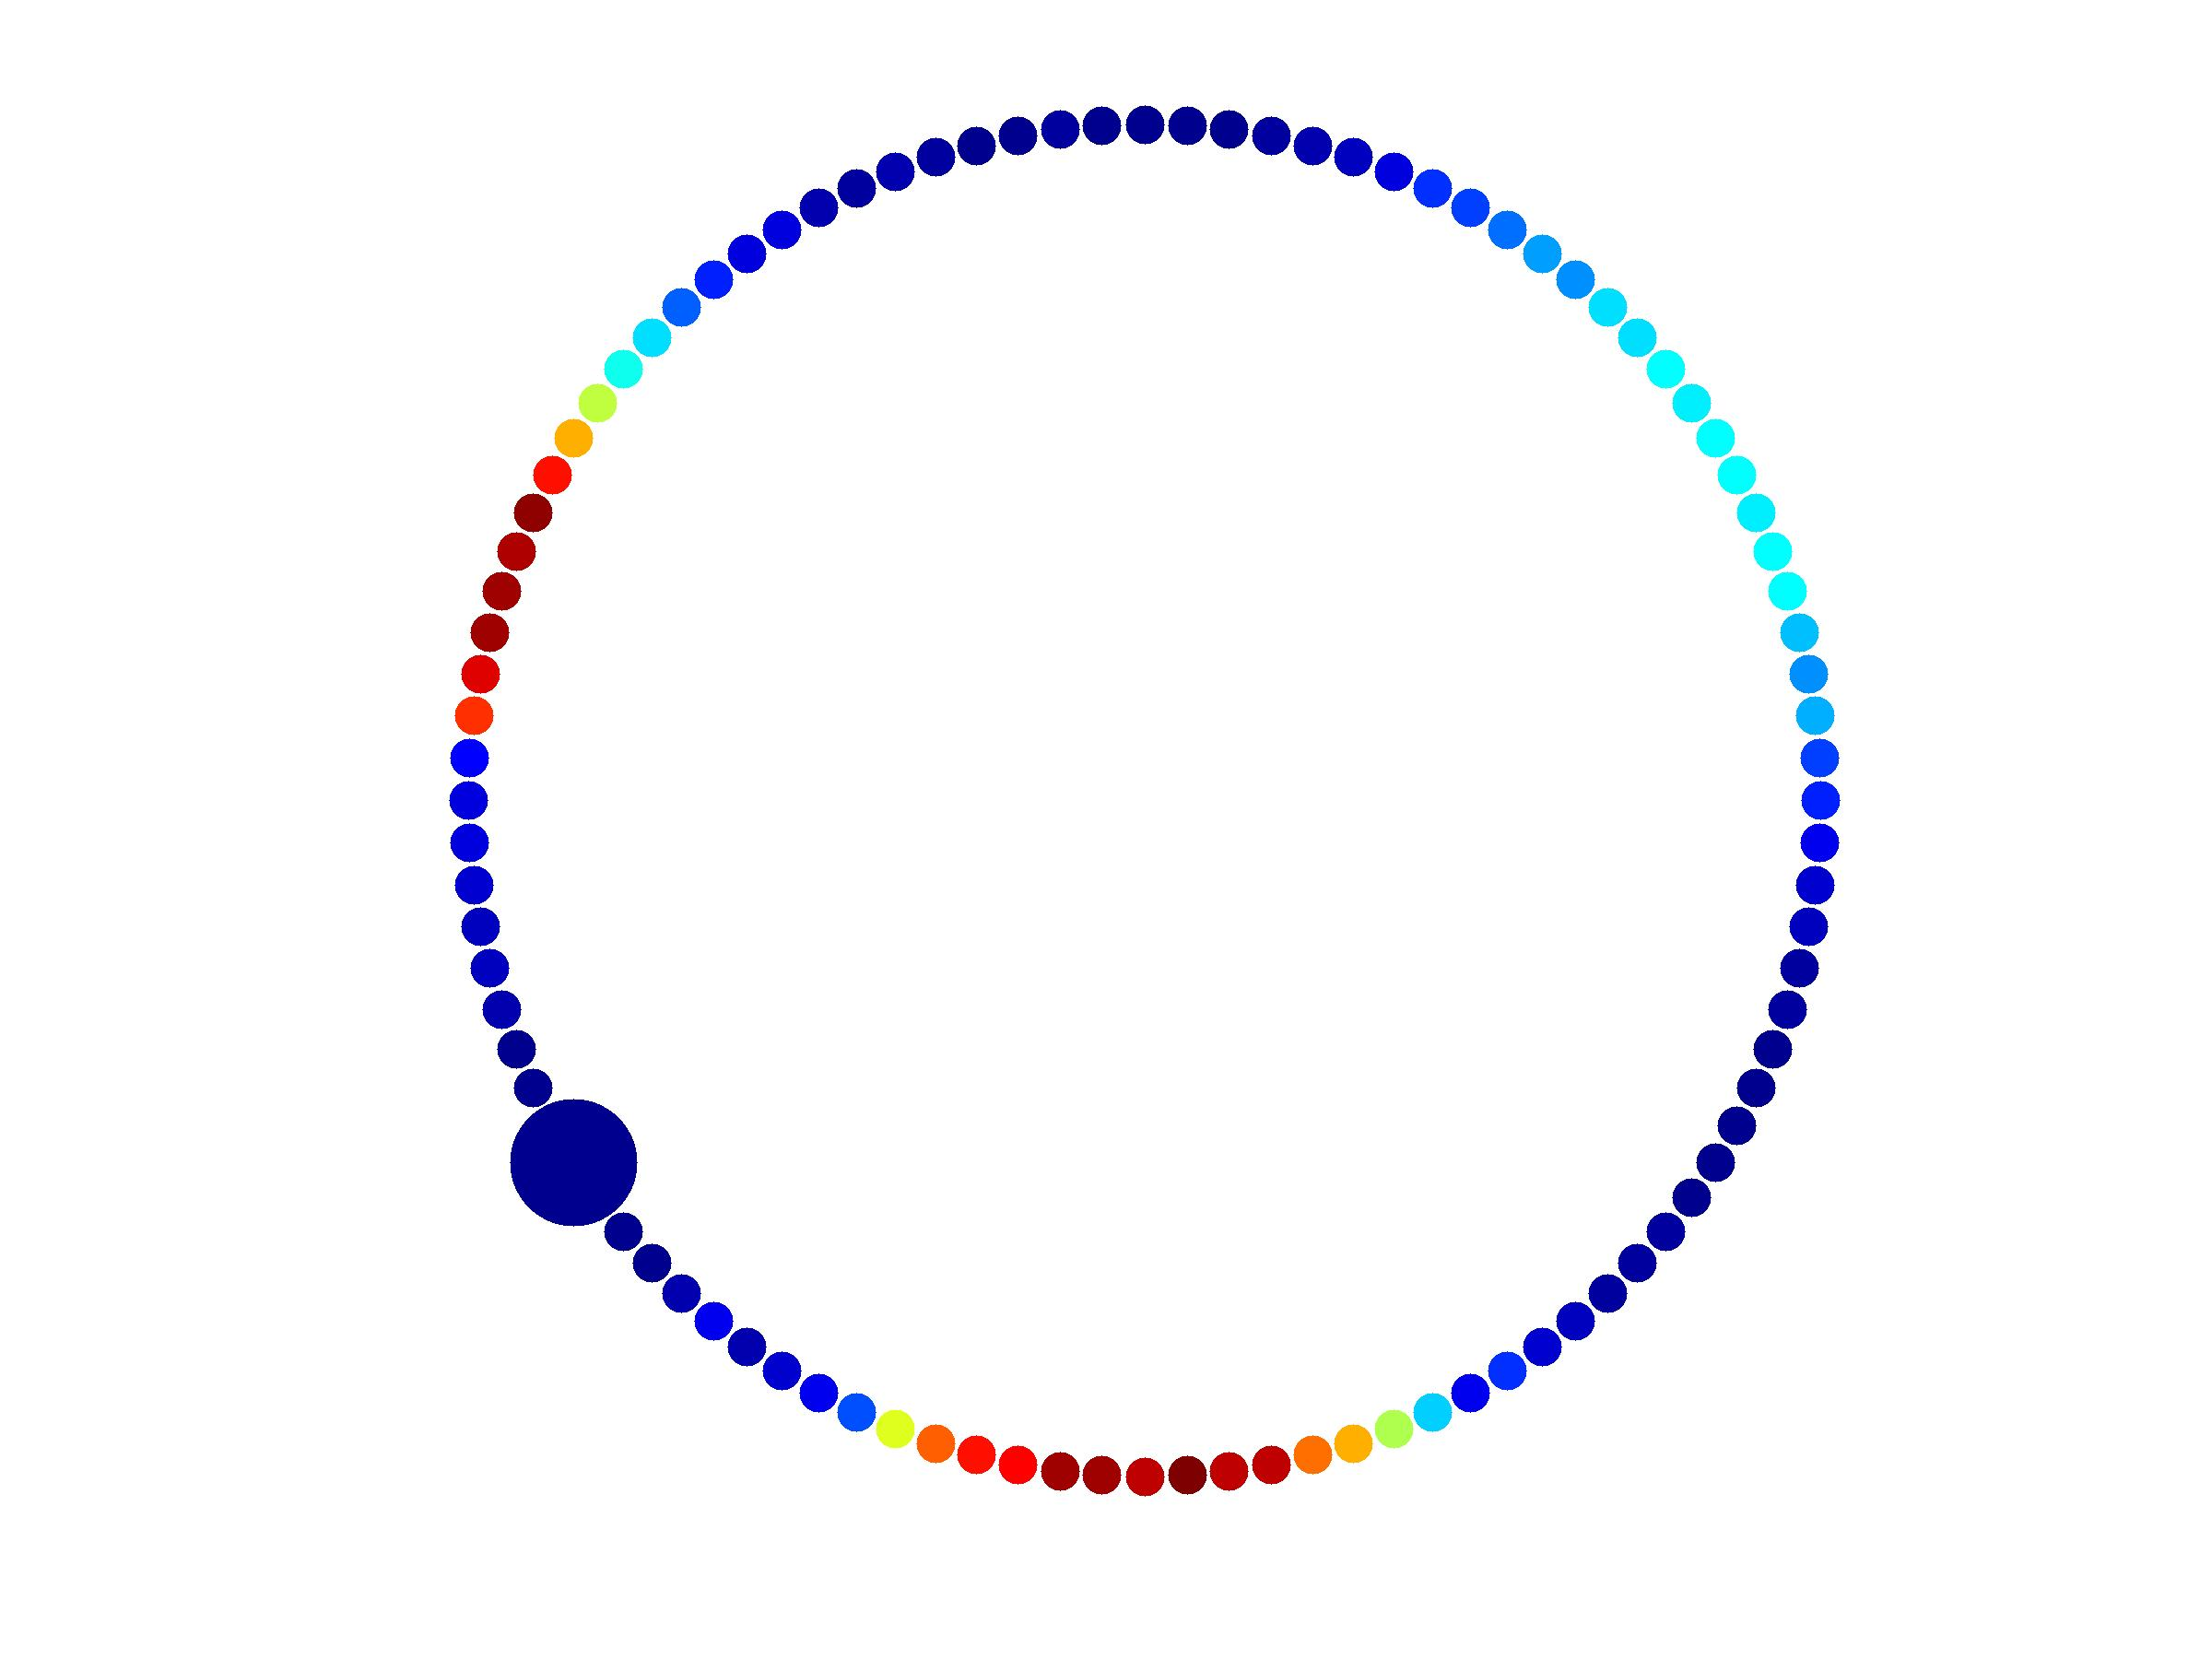
\includegraphics[width=0.45\textwidth]{../SIAM_DS_2013/drosophila_rot1.jpg}
            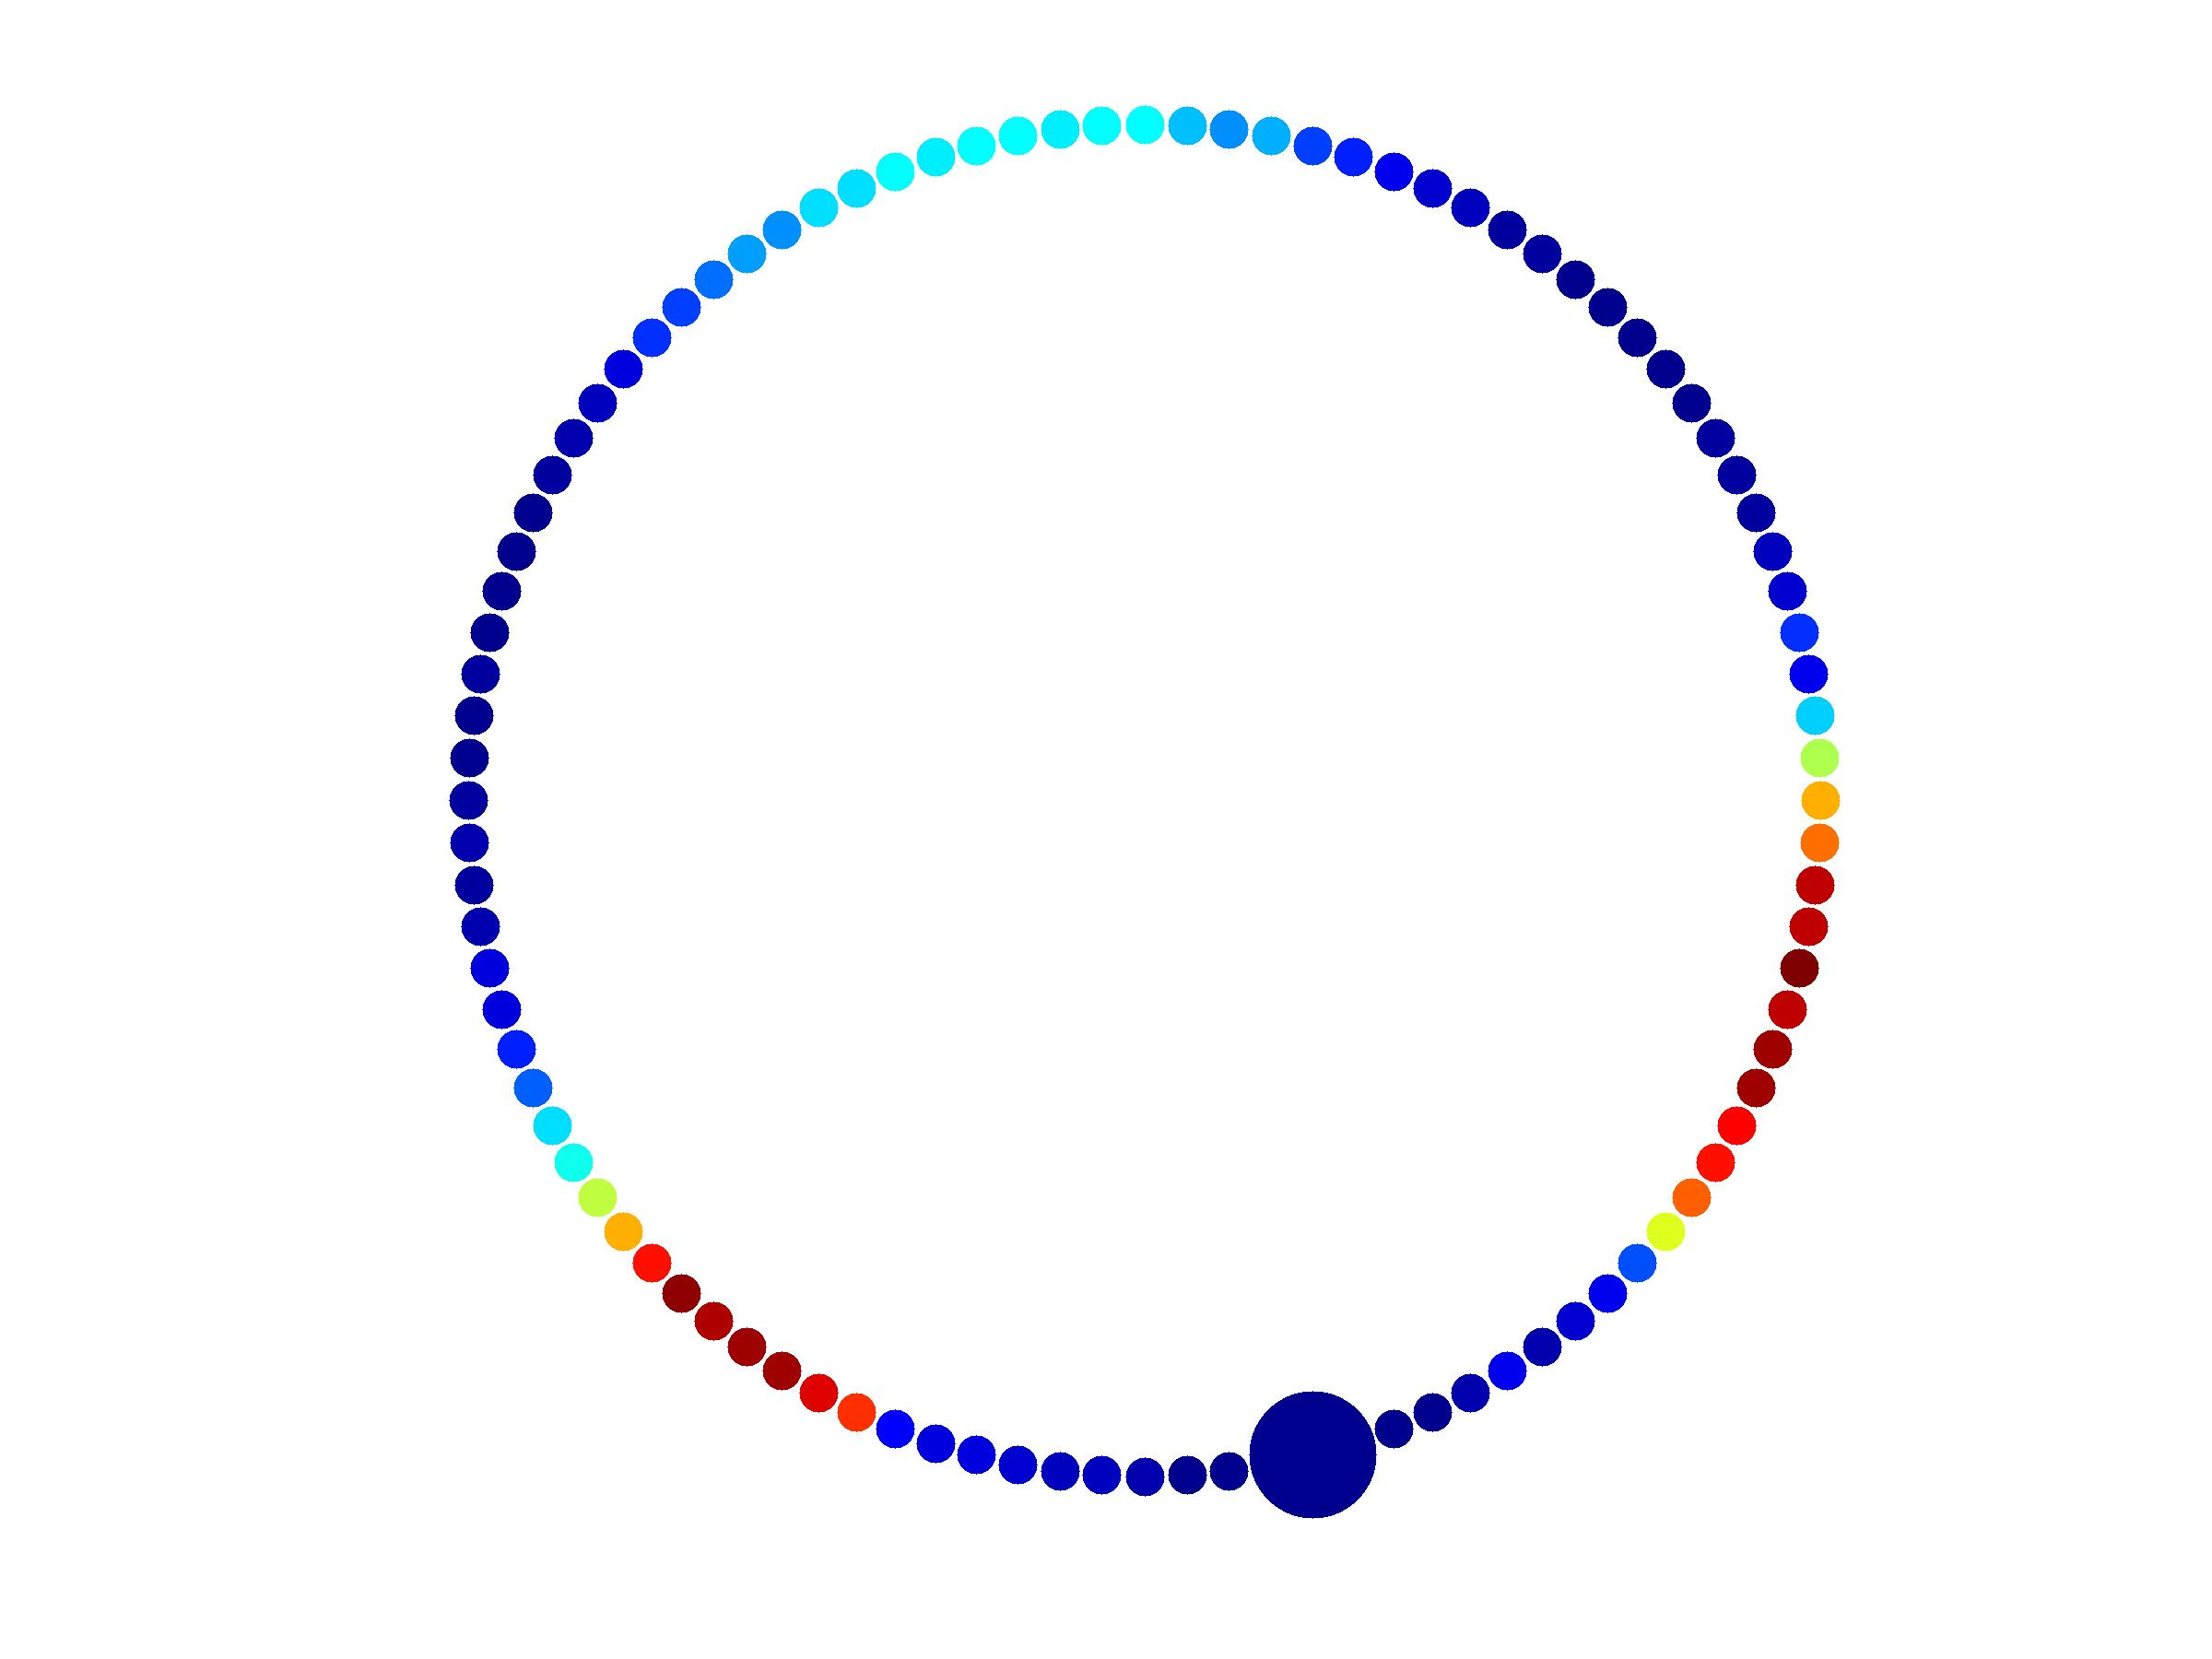
\includegraphics[width=0.45\textwidth]{../SIAM_DS_2013/drosophila_rot3.jpg}\\
			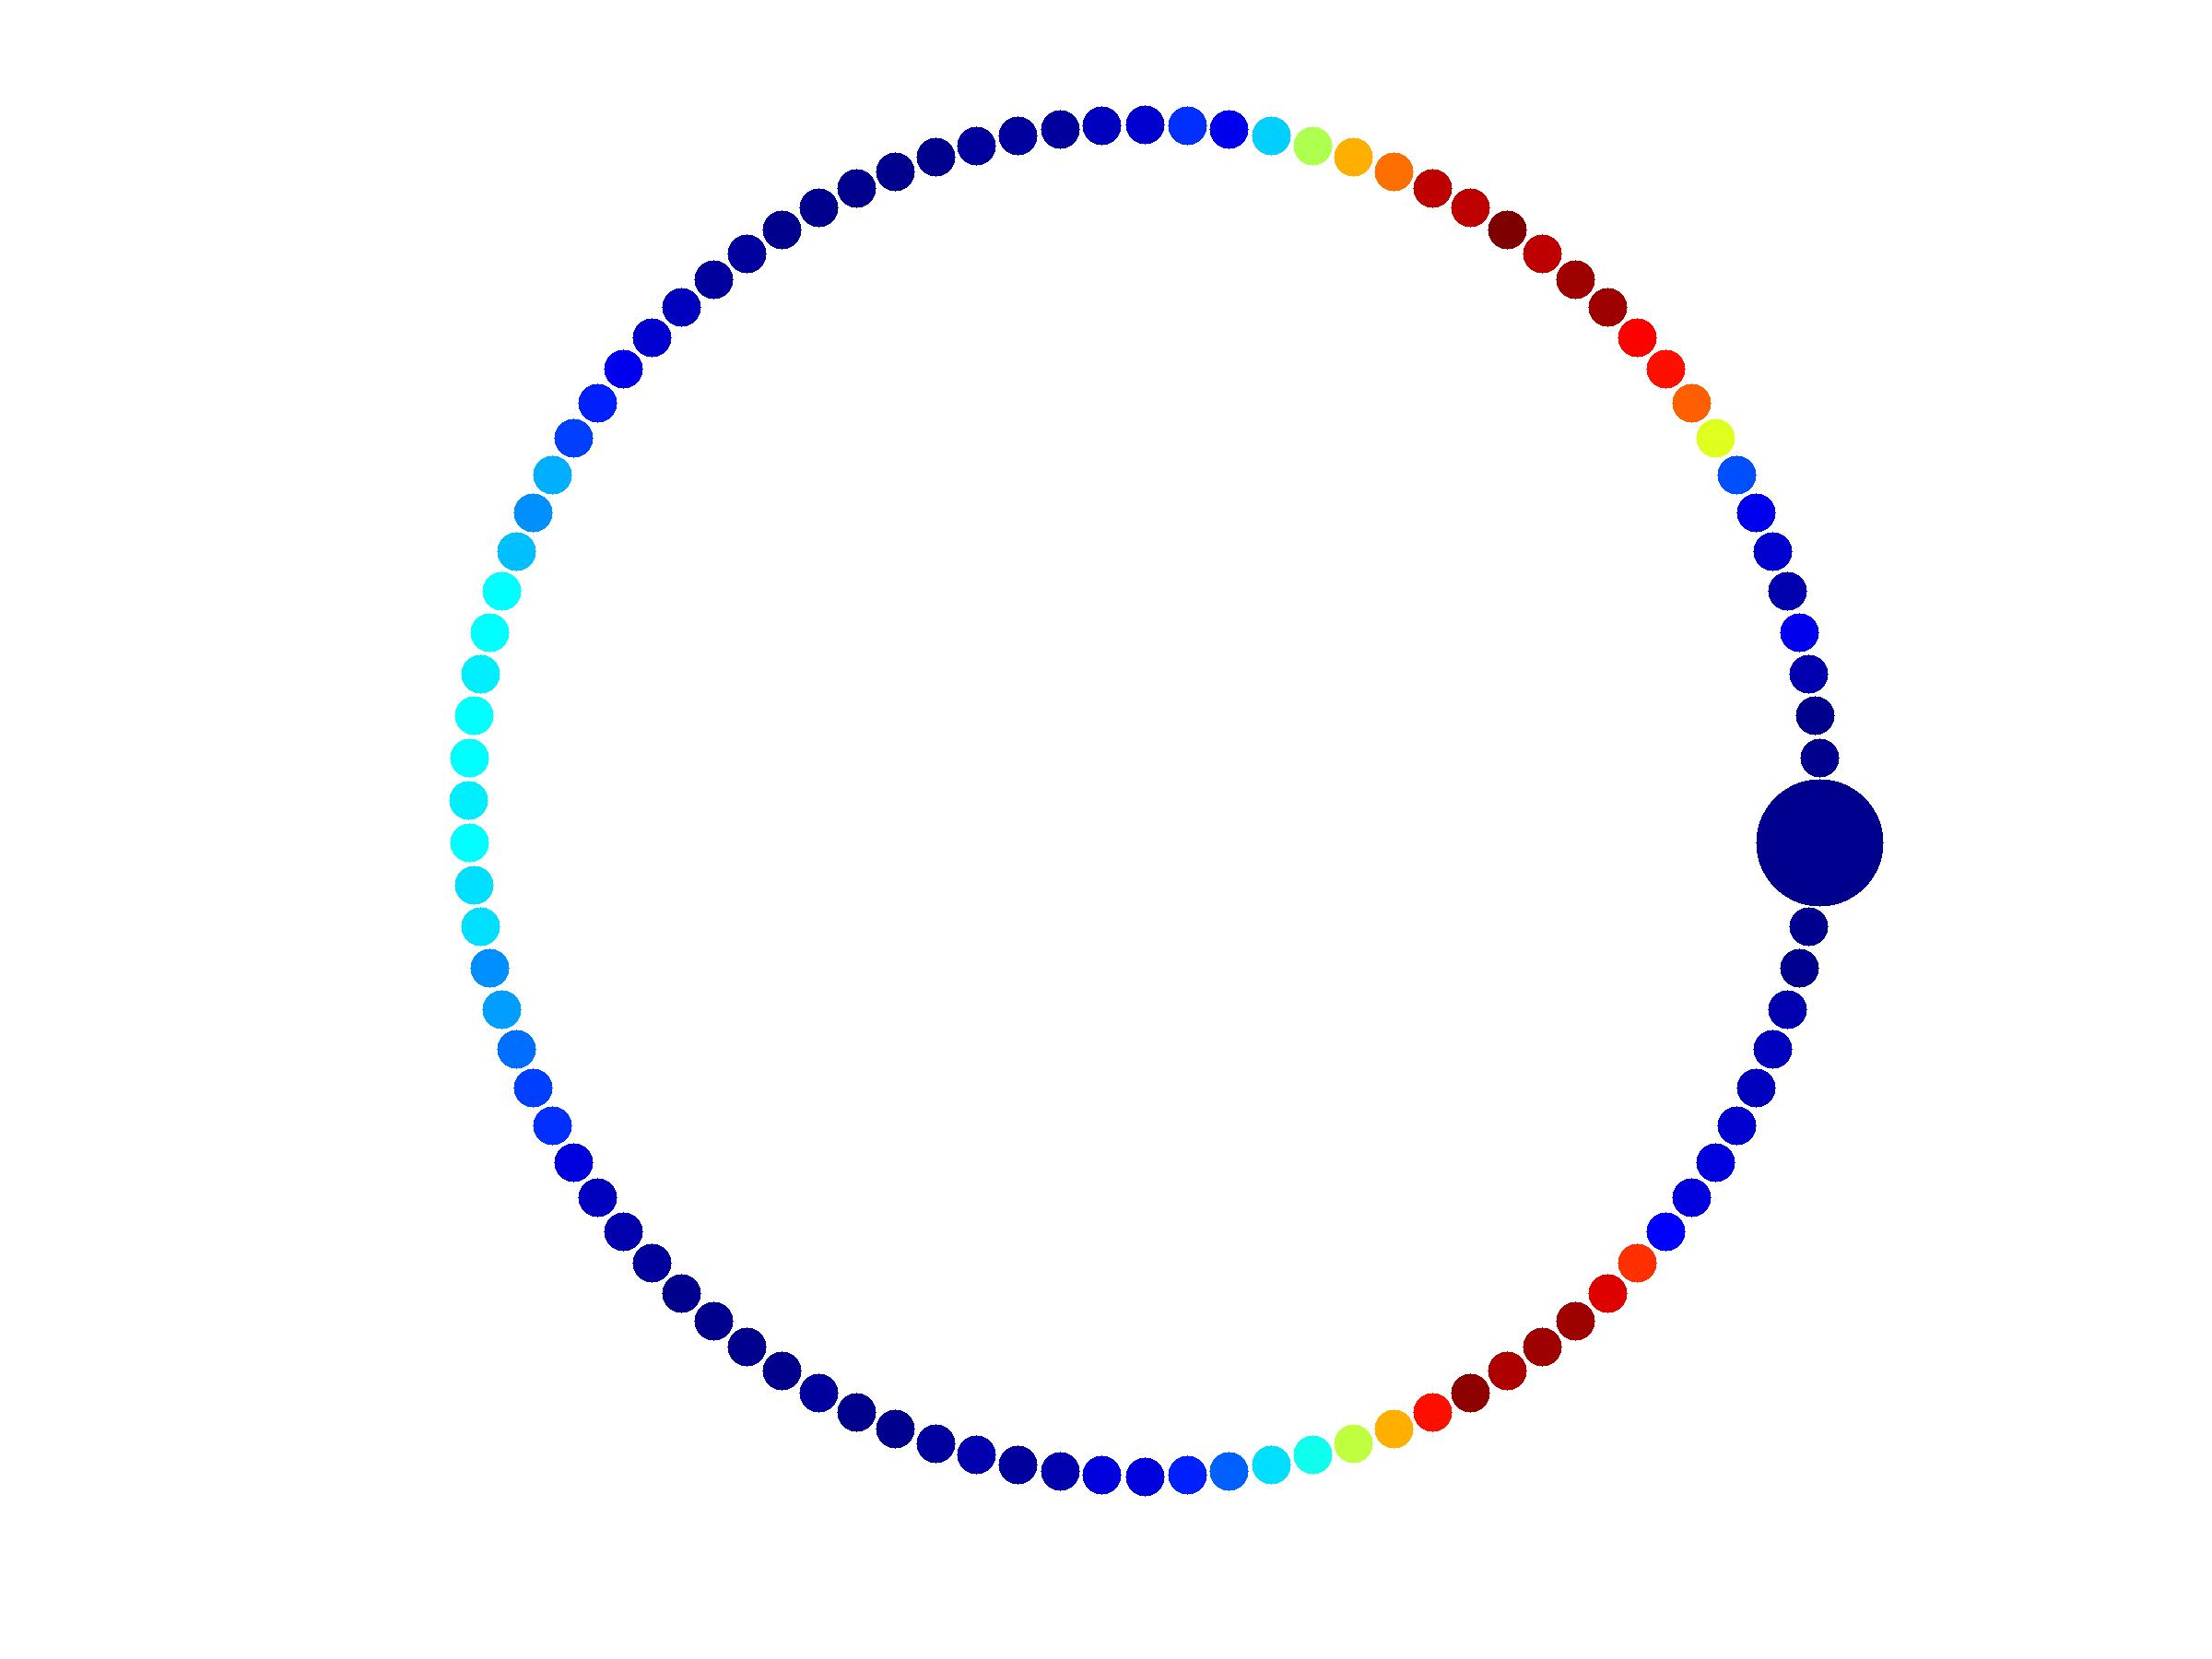
\includegraphics[width=0.45\textwidth]{../SIAM_DS_2013/drosophila_rot5.jpg}
            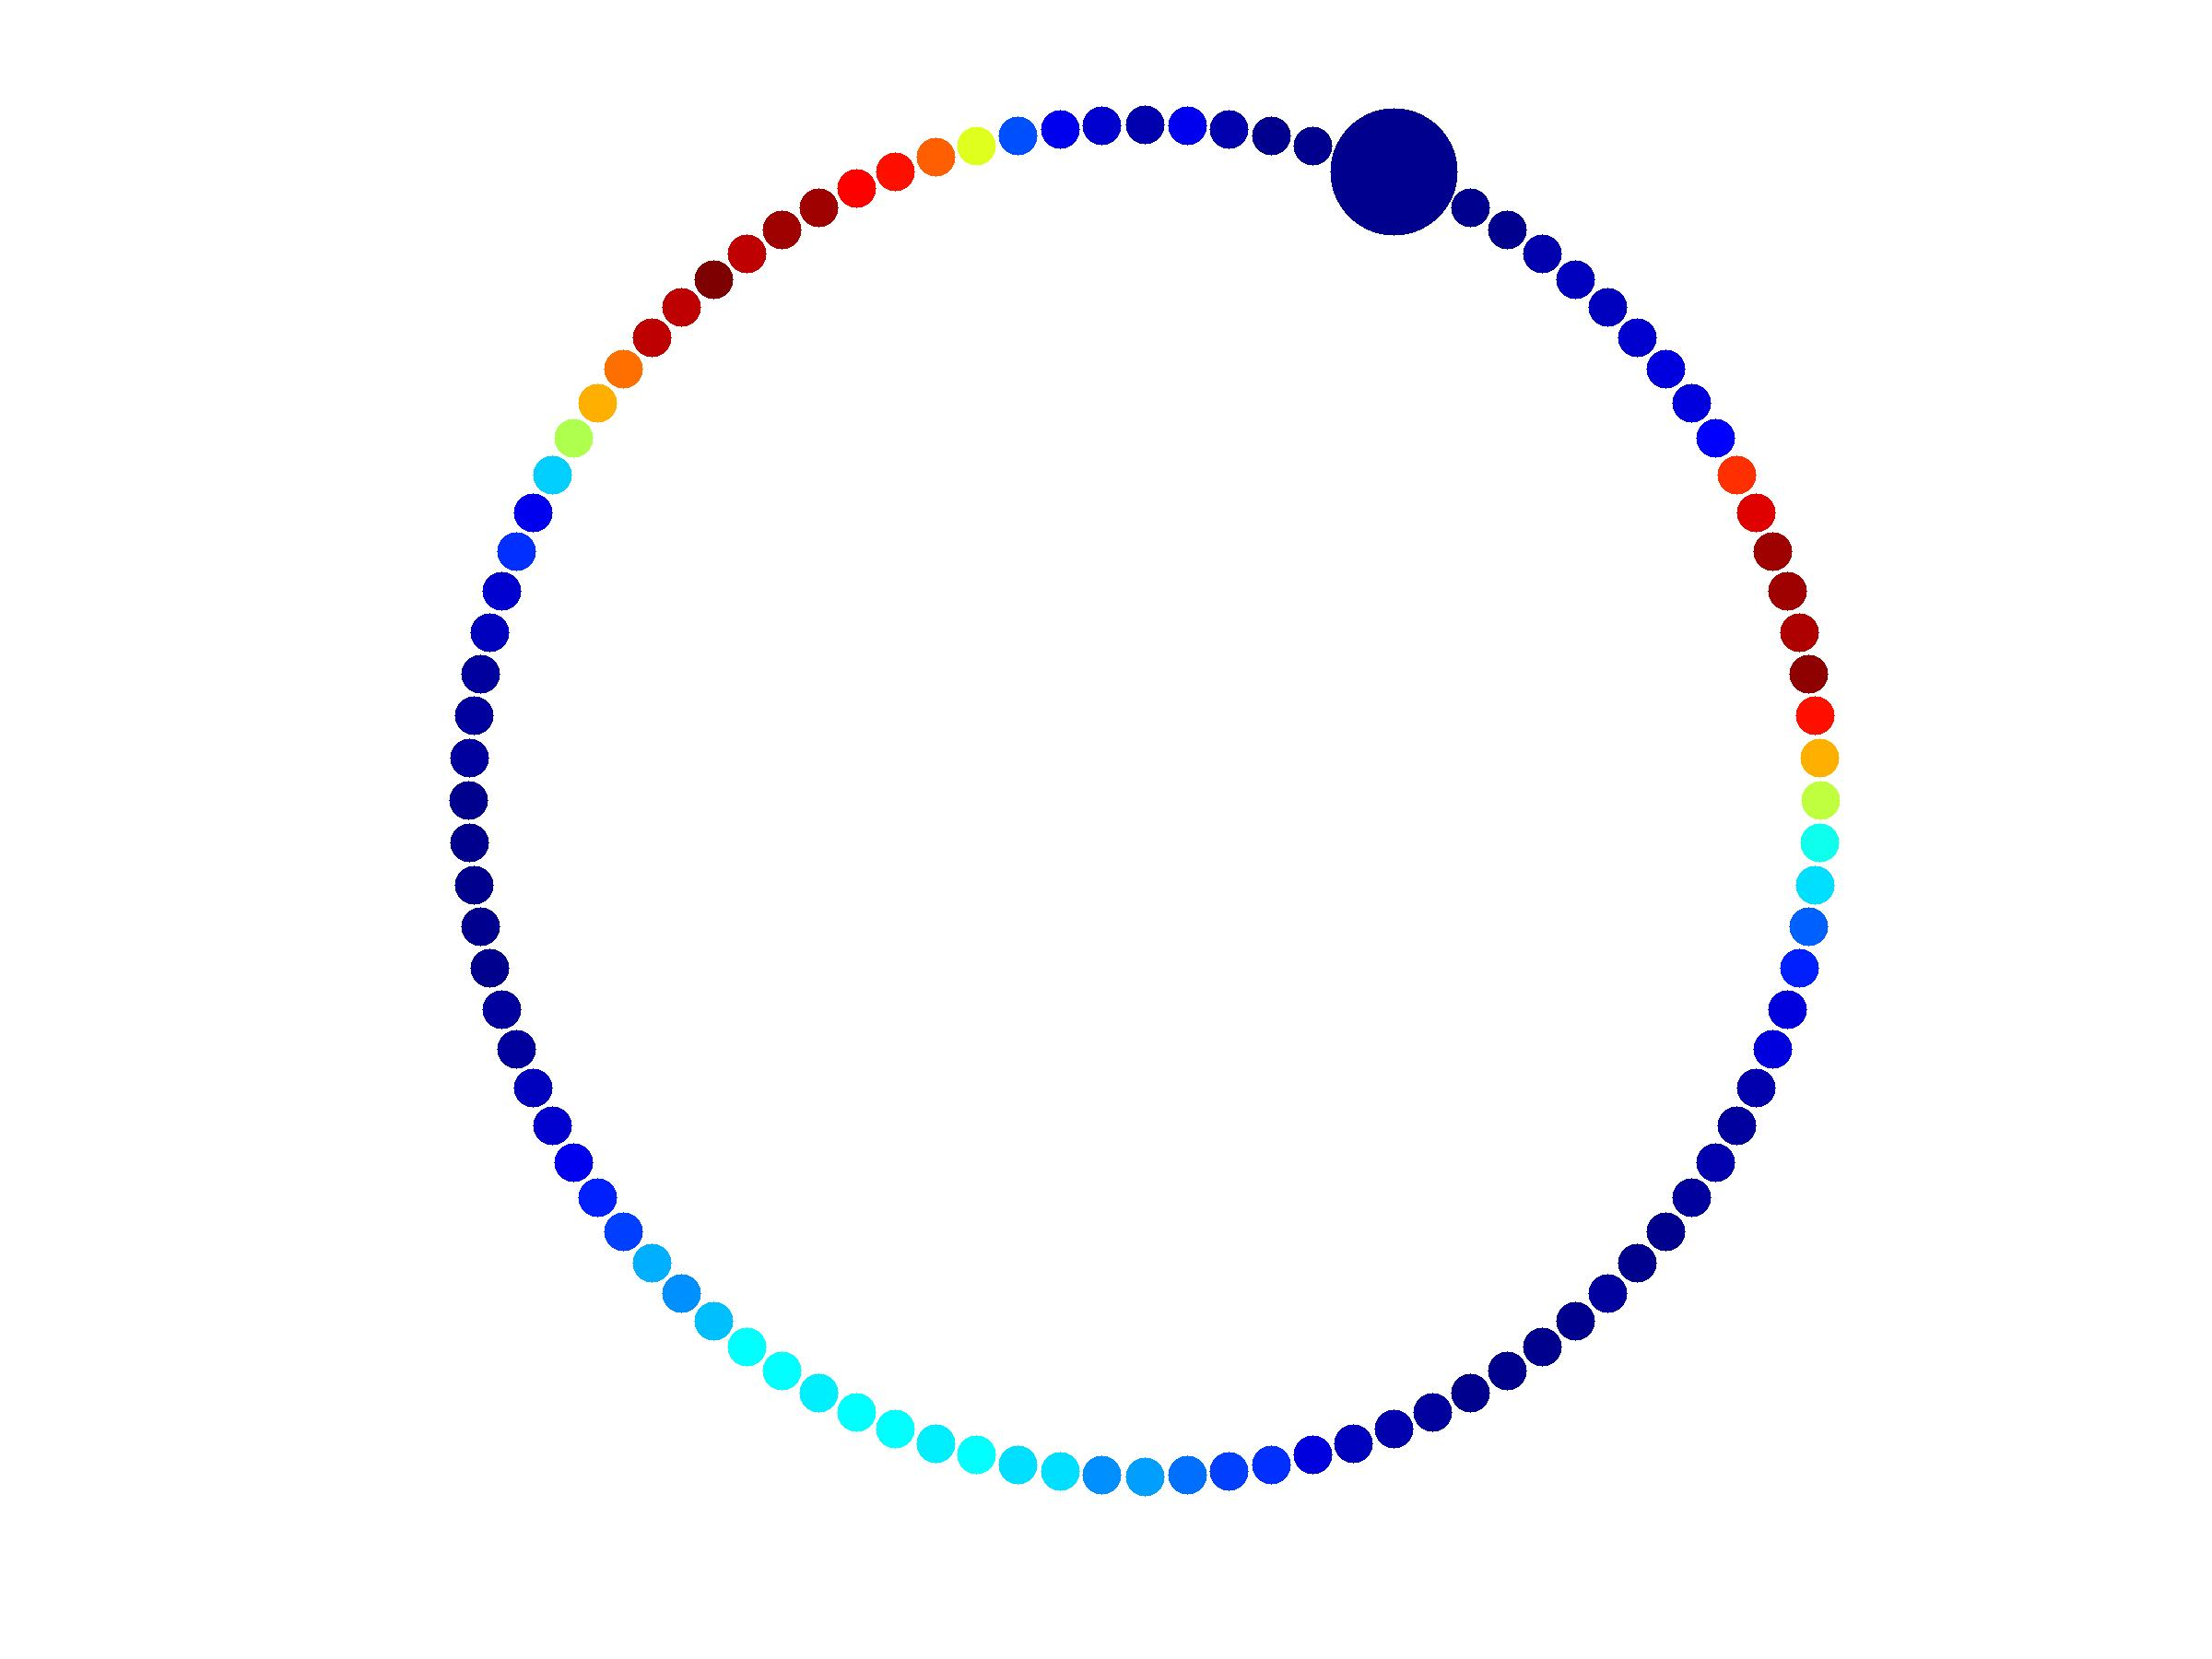
\includegraphics[width=0.45\textwidth]{../SIAM_DS_2013/drosophila_rot7.jpg}
            \end{minipage}};
            
            \node [right of=fig1, node distance=0.35\textwidth] (fig2) {
            \begin{minipage}{0.25\textwidth}
            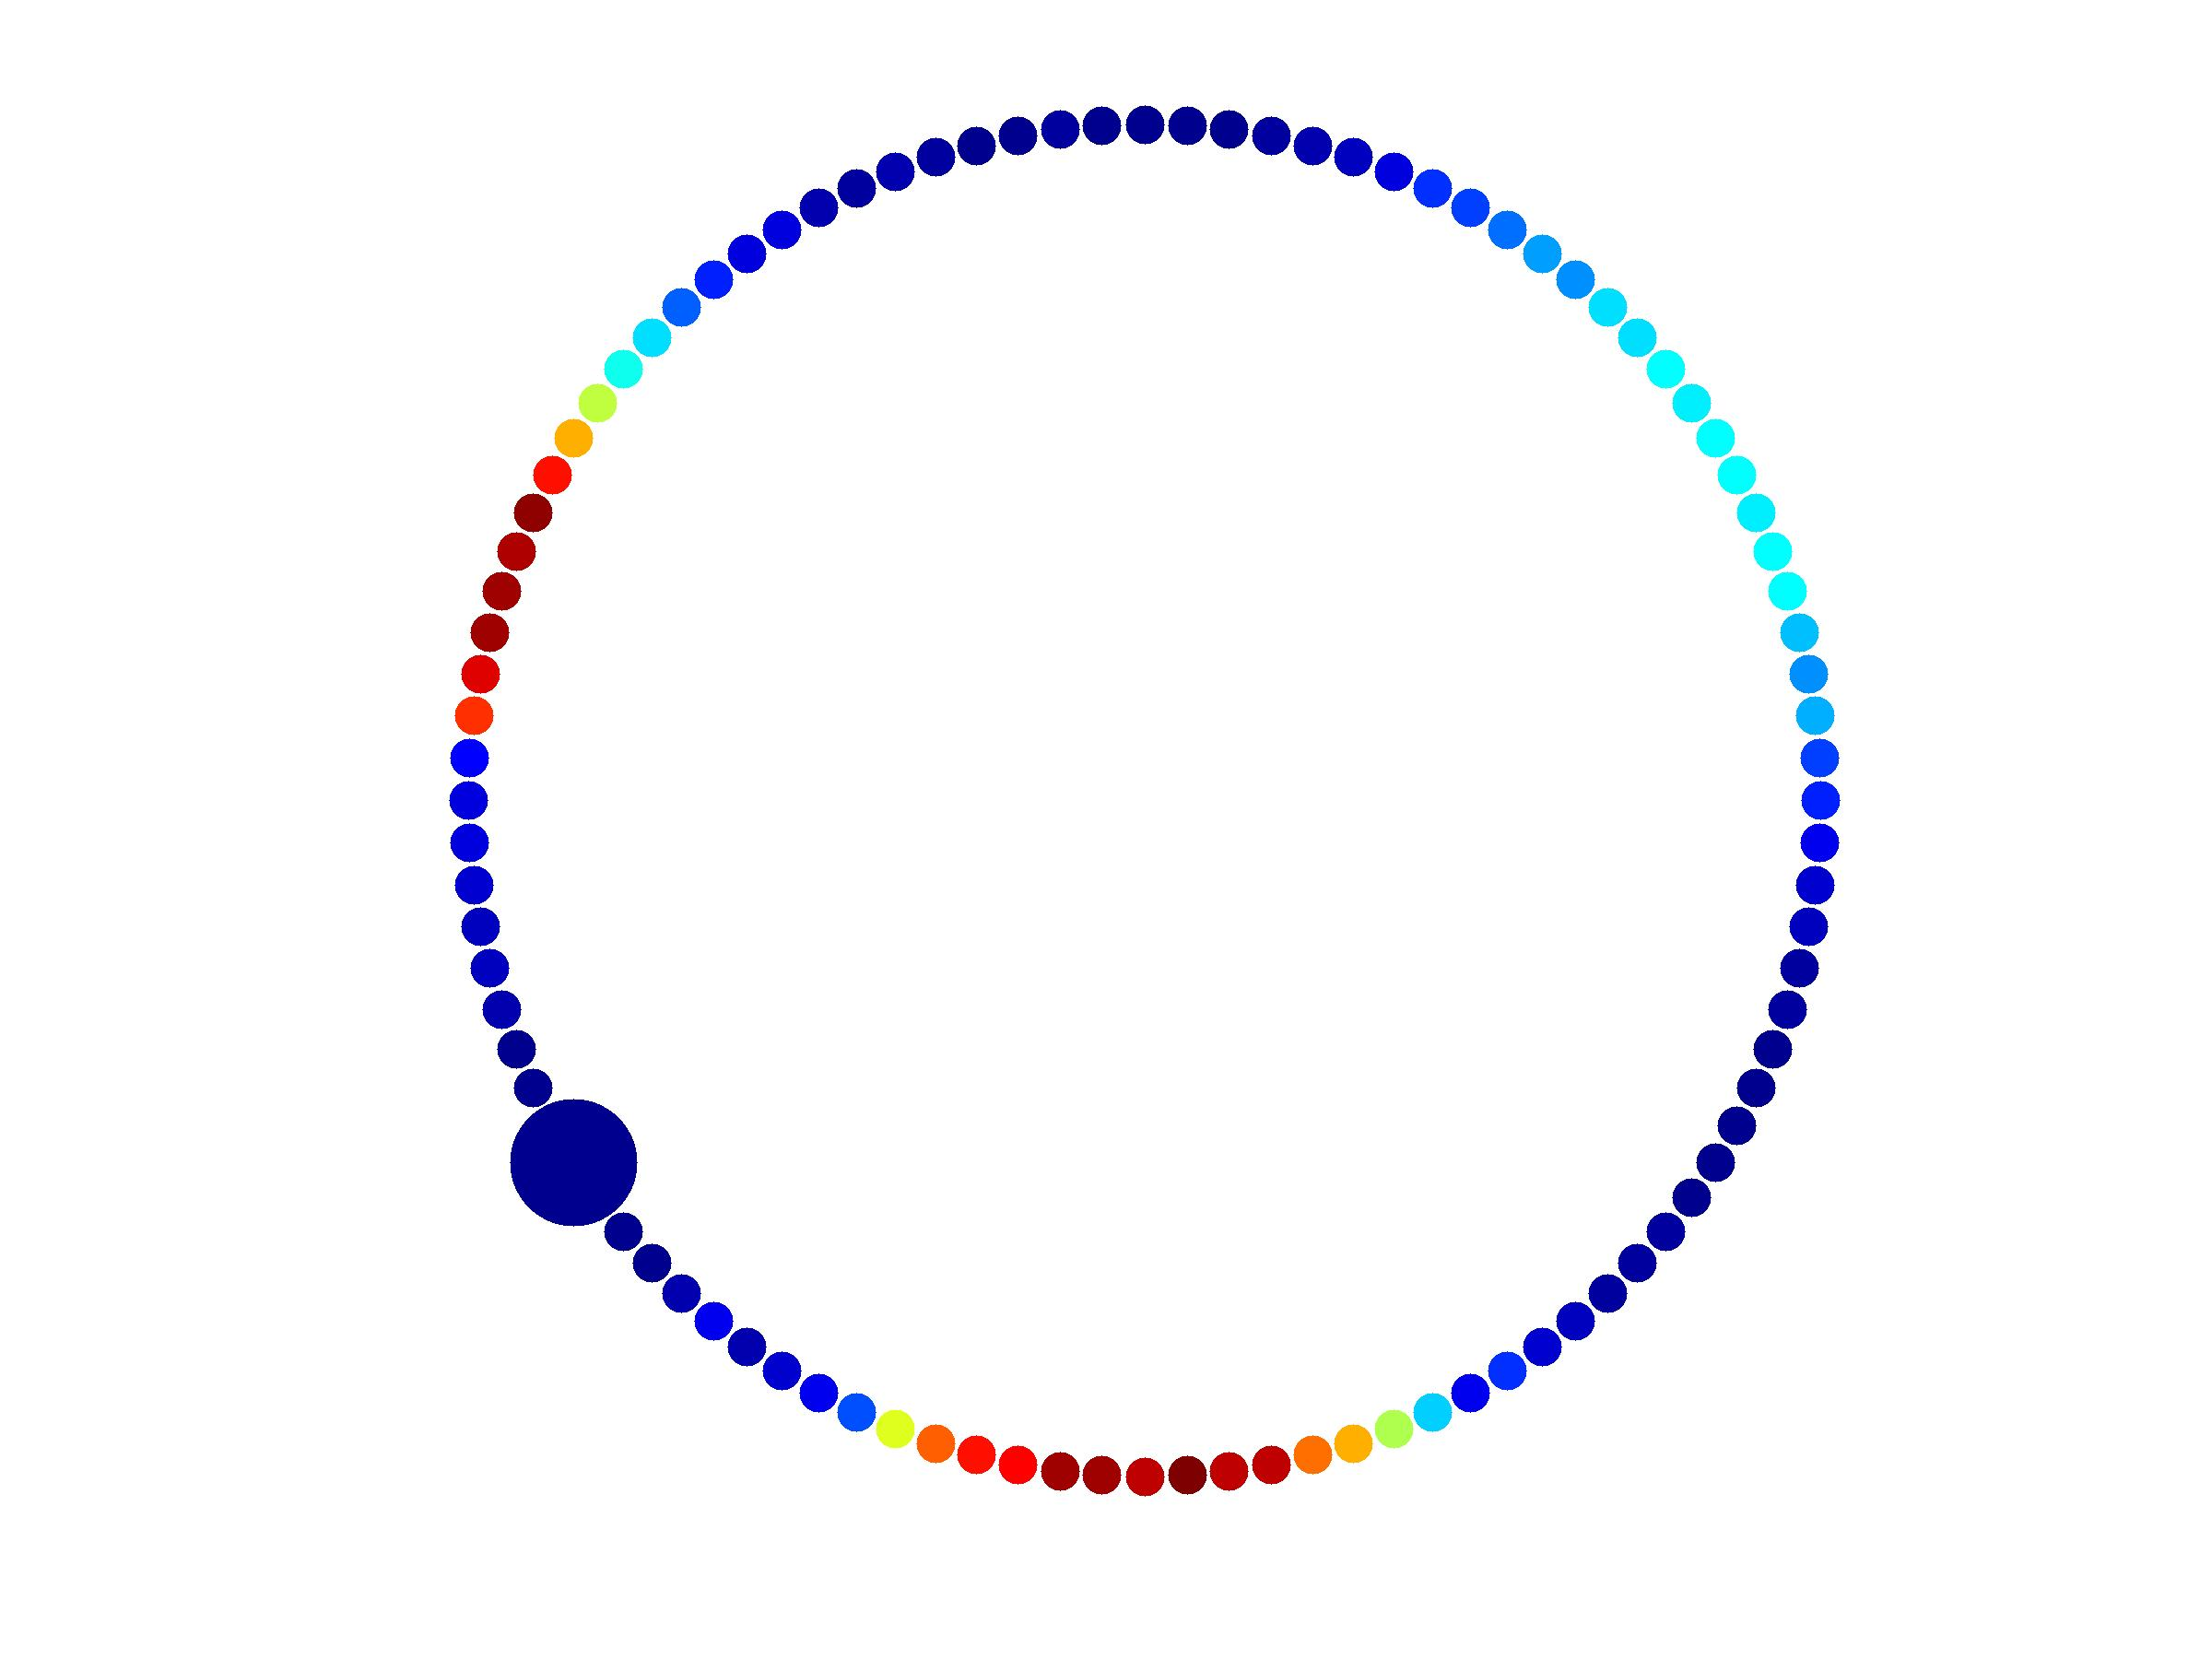
\includegraphics[width=0.45\textwidth]{../SIAM_DS_2013/drosophila_rot1.jpg}
            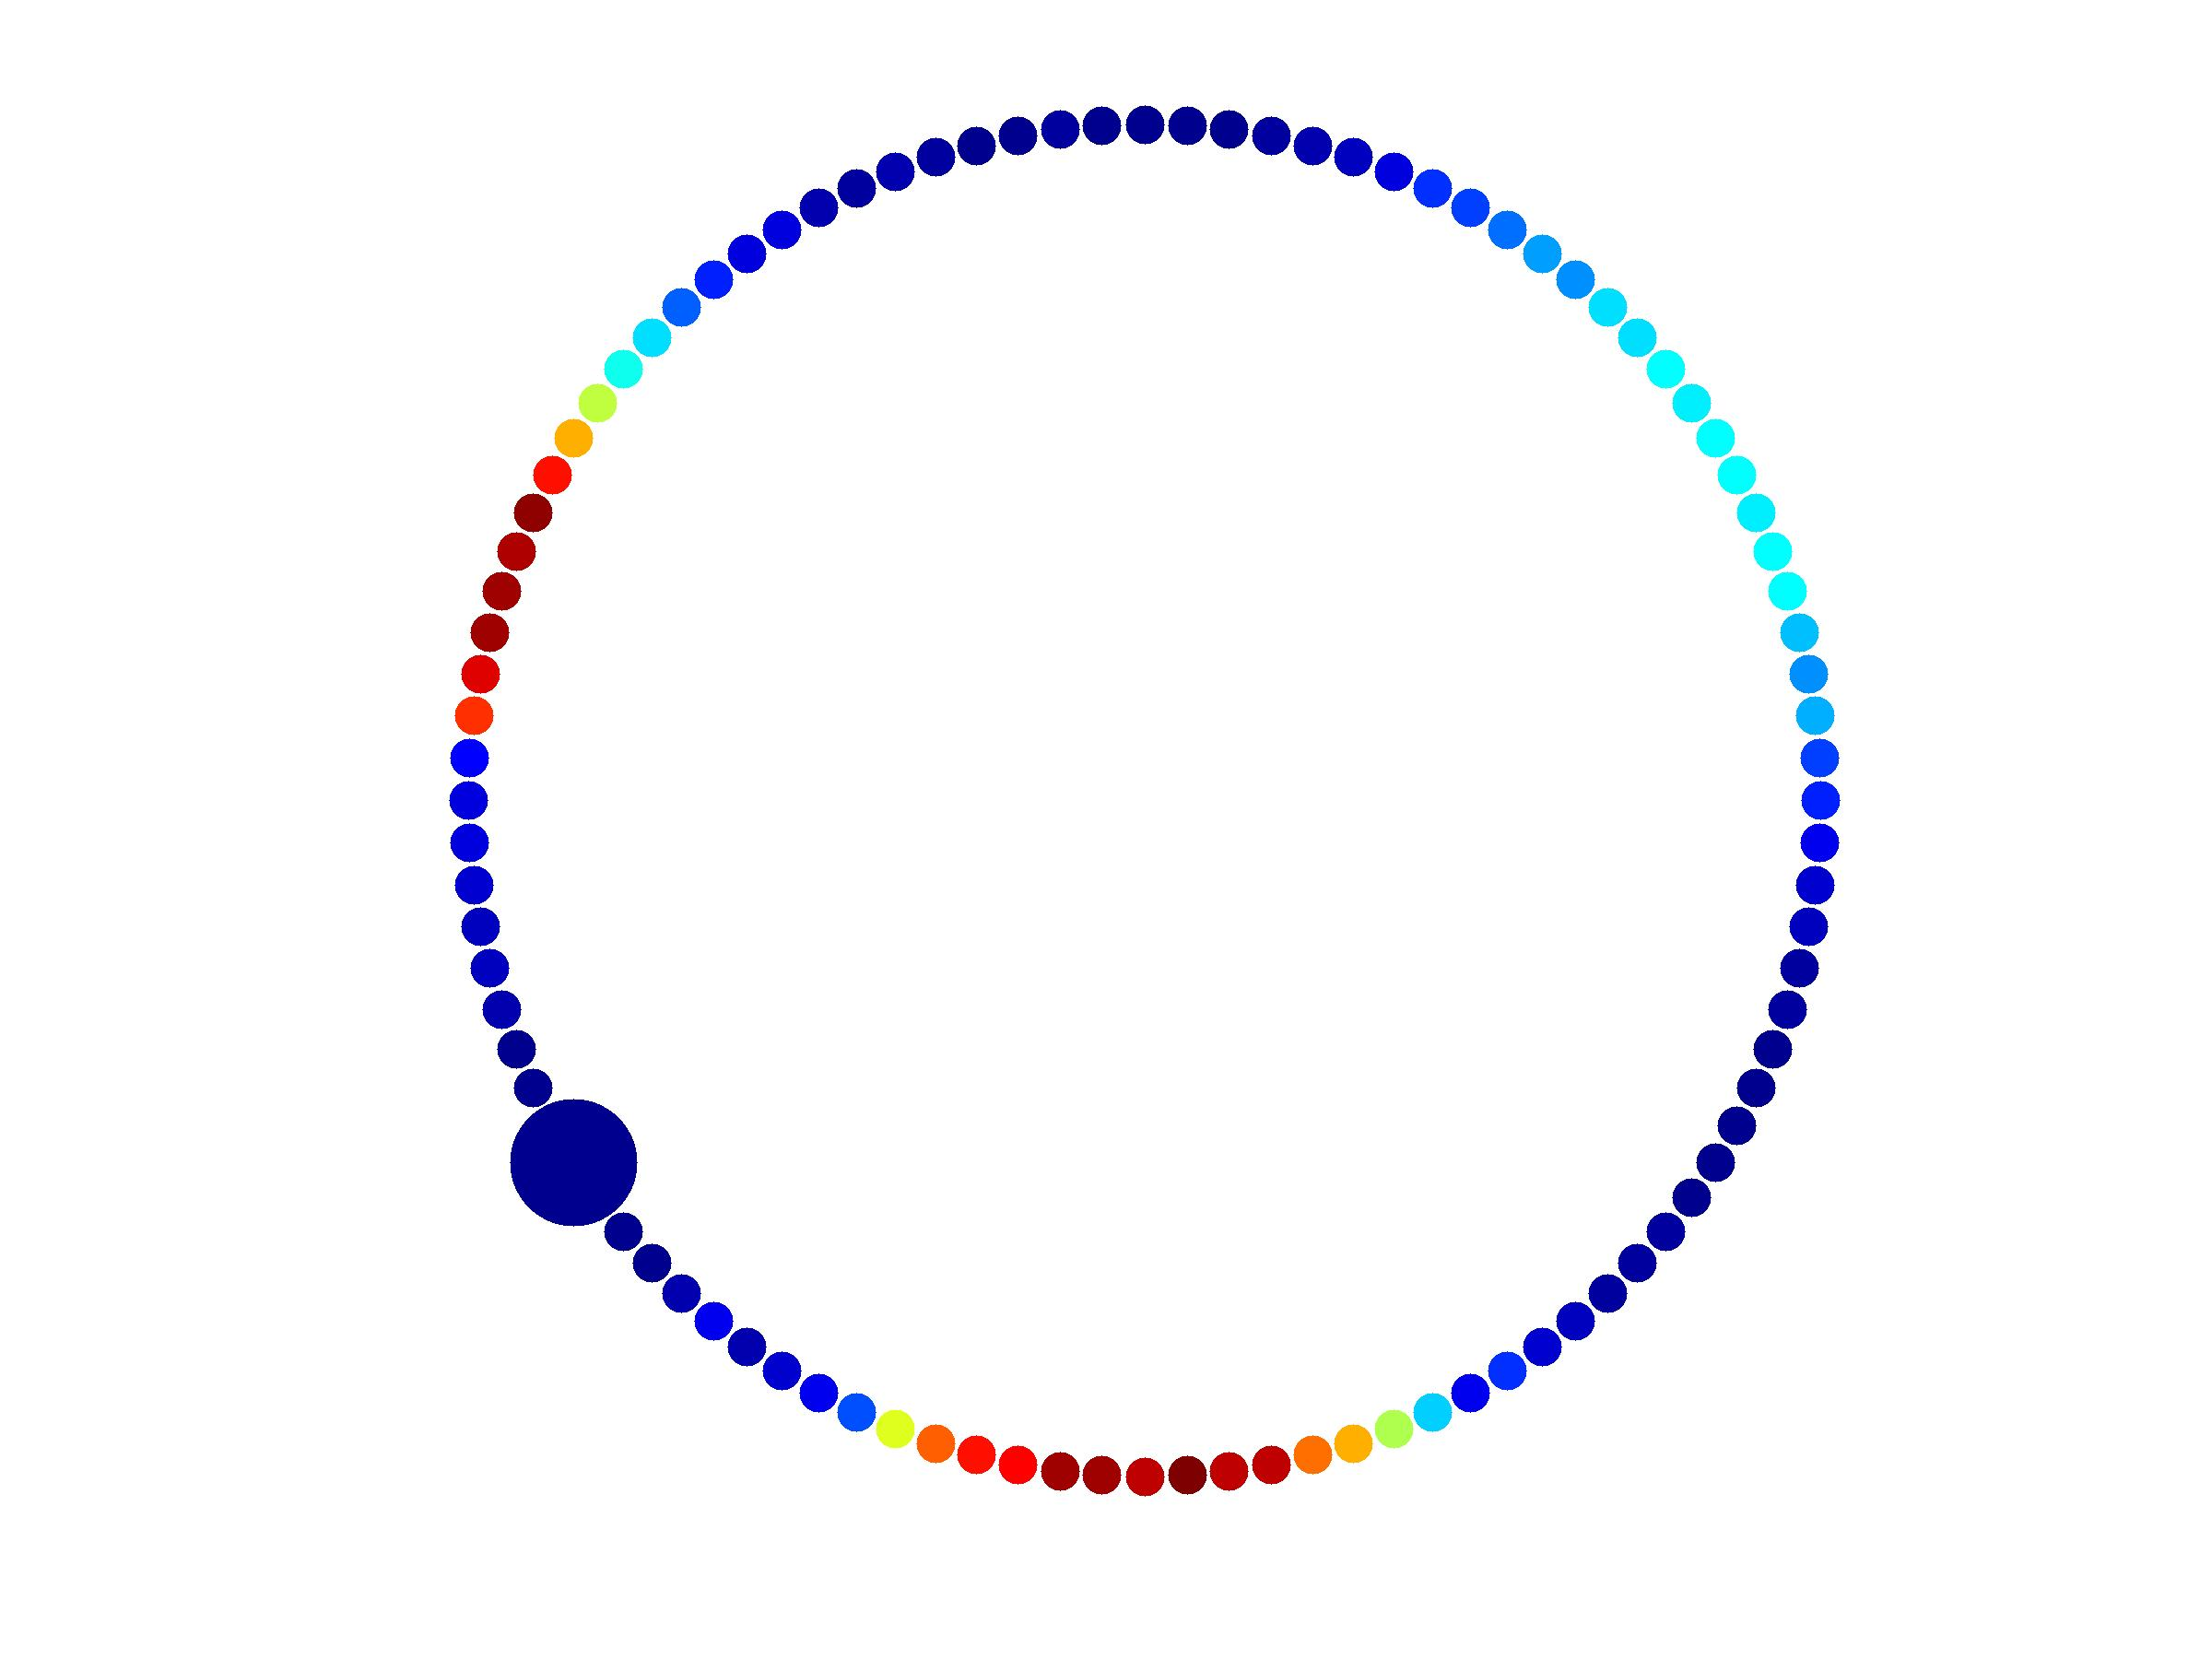
\includegraphics[width=0.45\textwidth]{../SIAM_DS_2013/drosophila_rot1.jpg}\\
            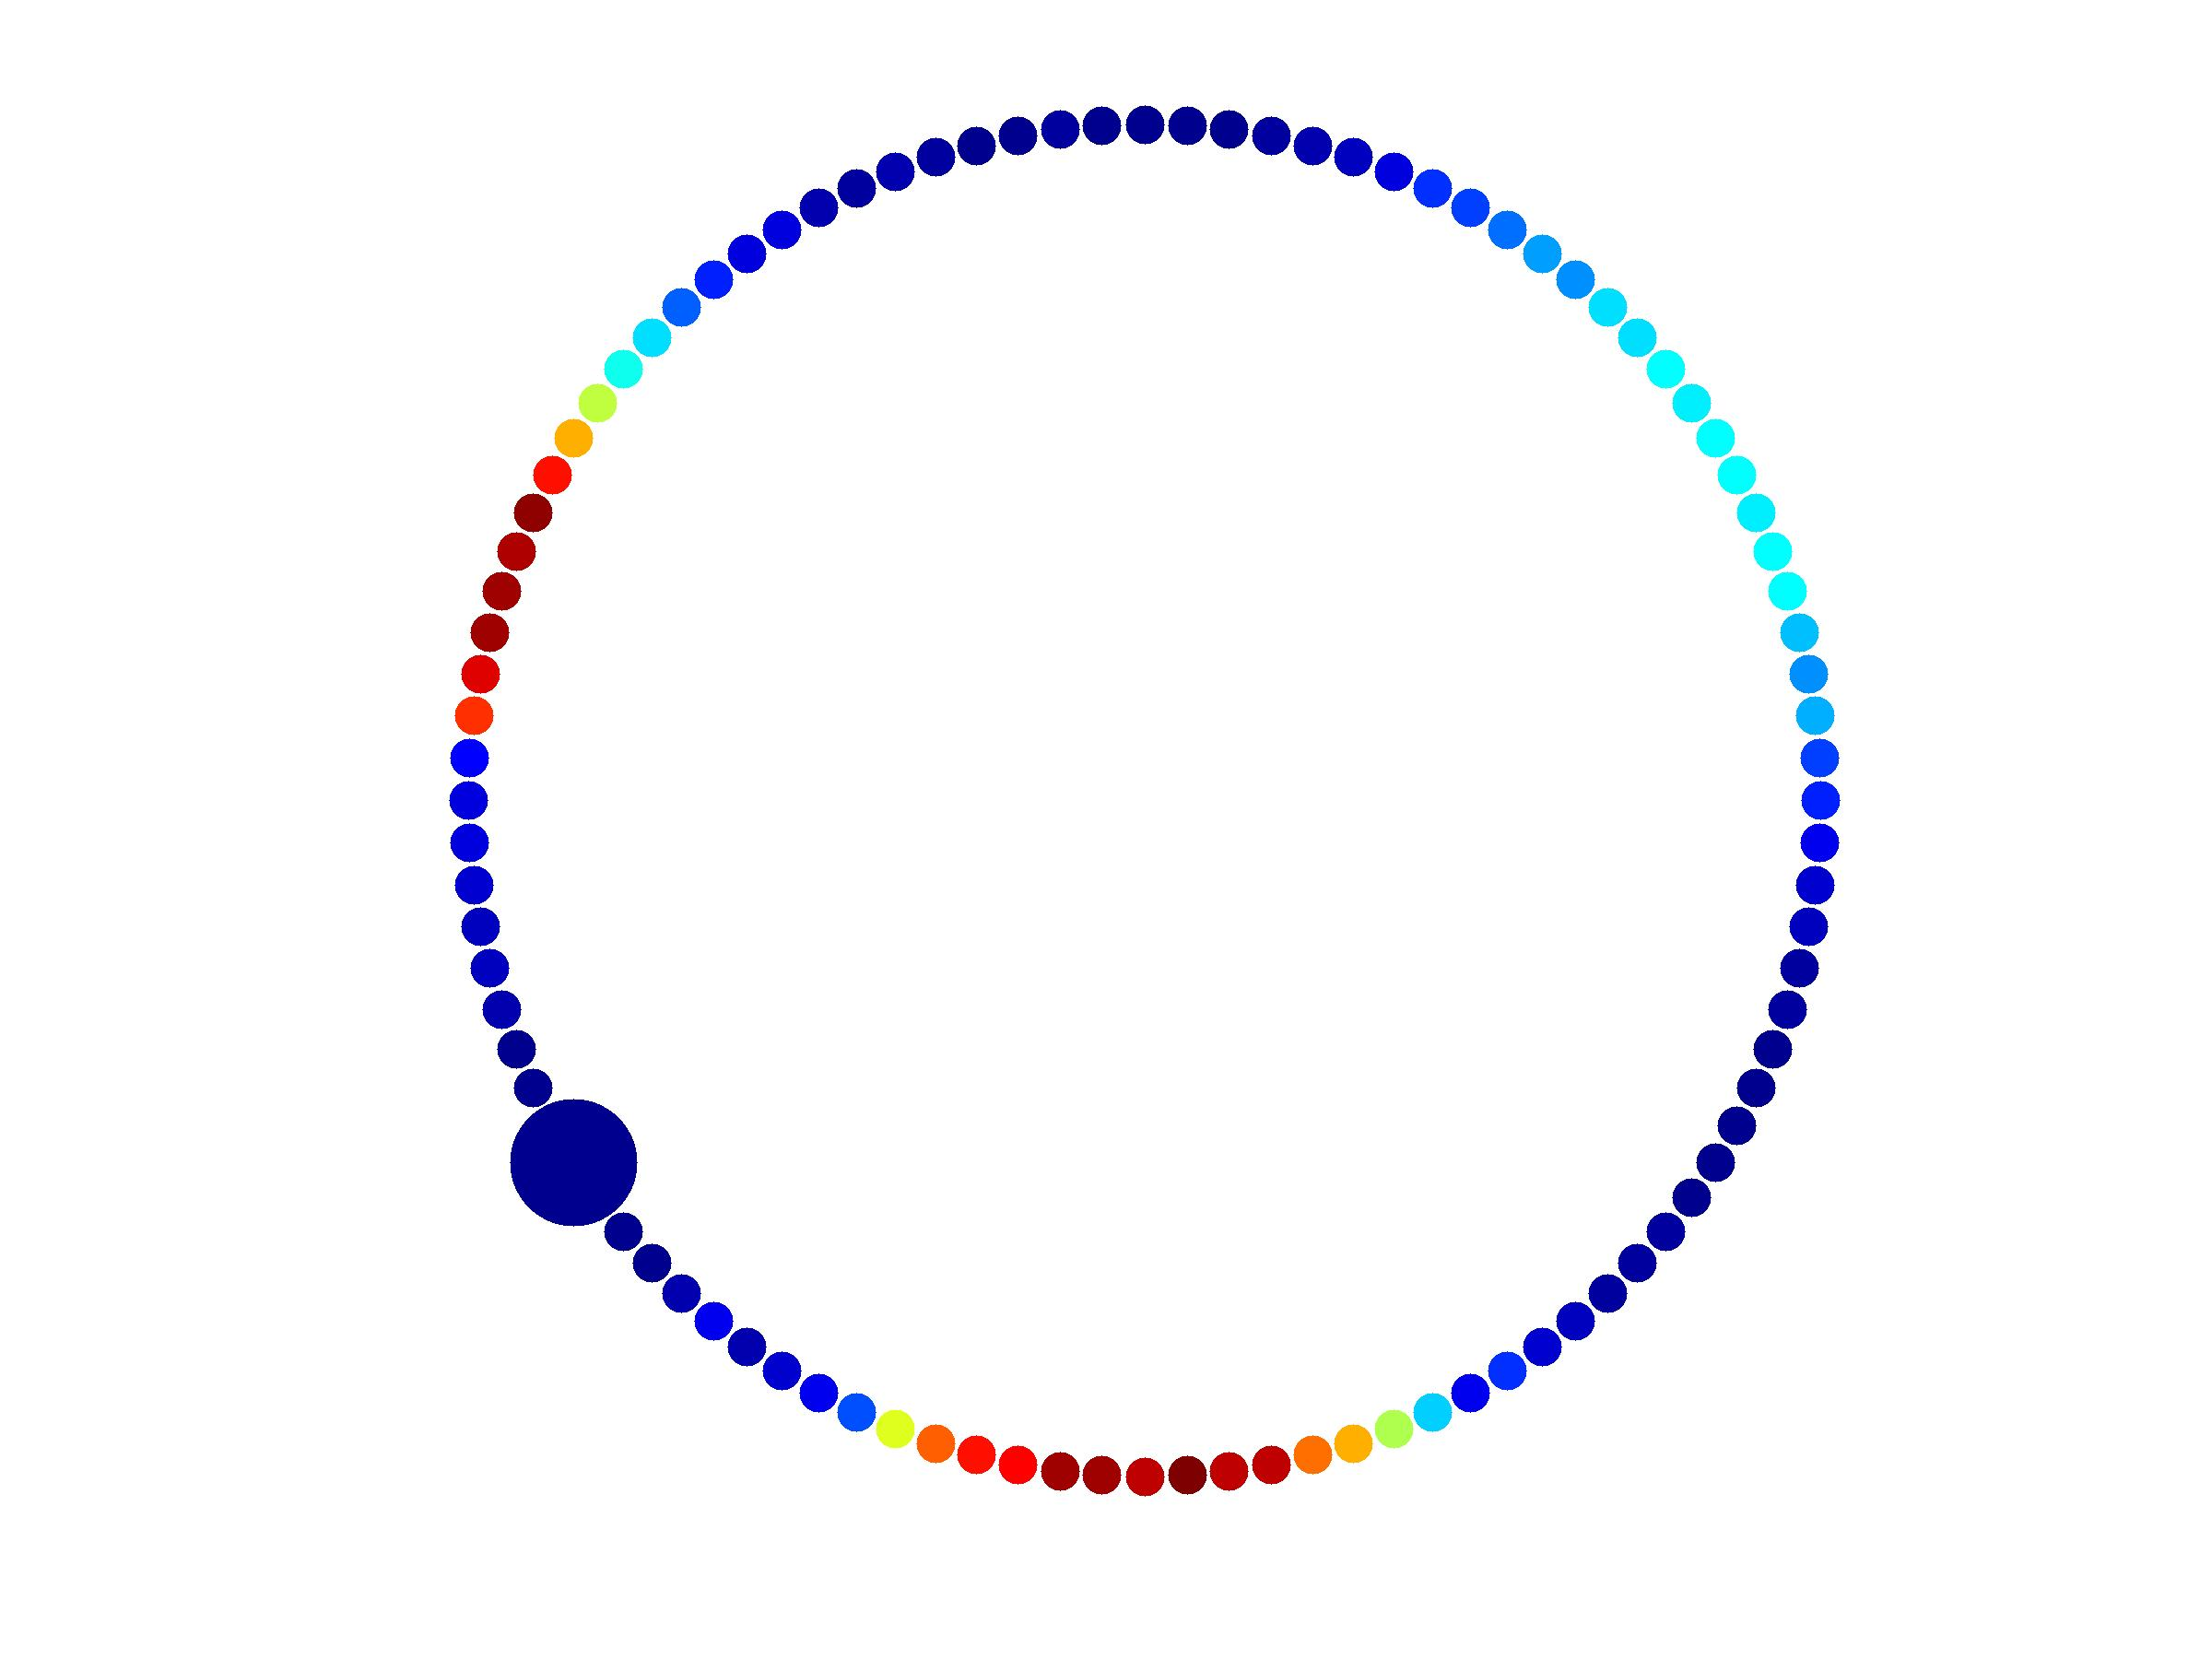
\includegraphics[width=0.45\textwidth]{../SIAM_DS_2013/drosophila_rot1.jpg}
            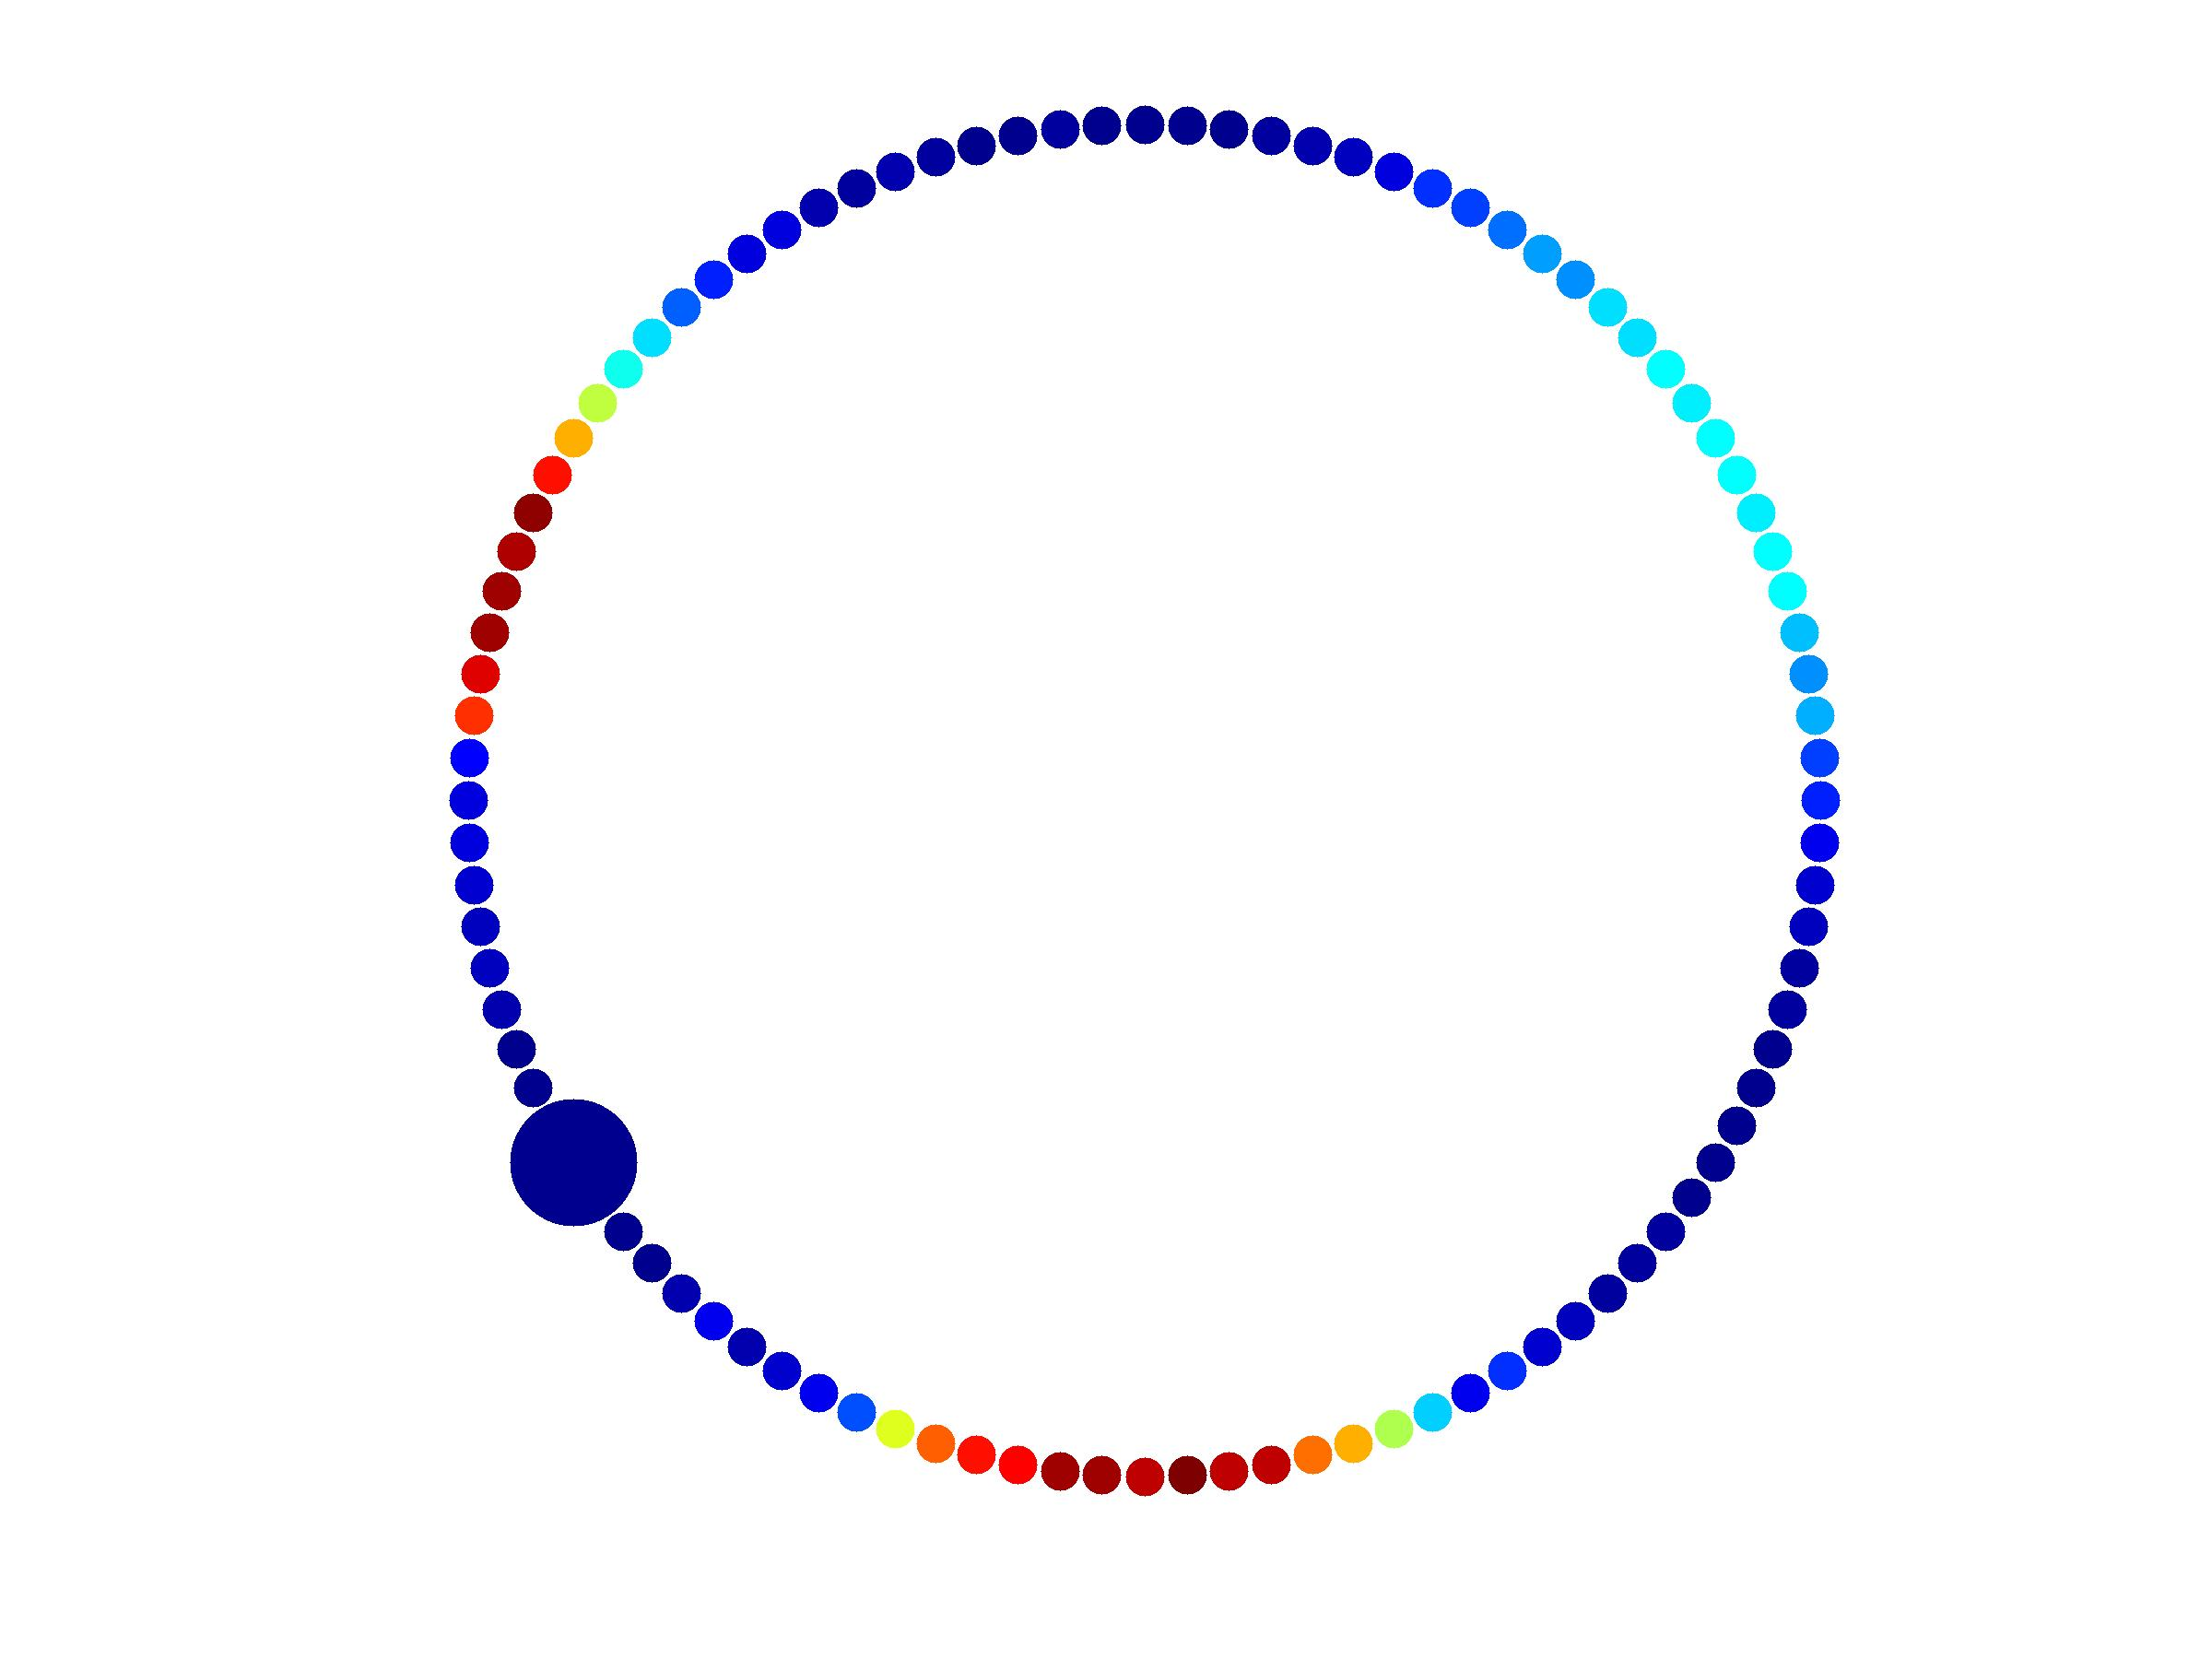
\includegraphics[width=0.45\textwidth]{../SIAM_DS_2013/drosophila_rot1.jpg}
            \end{minipage}};
            \draw [->] (fig1.east) -- (fig2.west);
        \end{tikzpicture}
	\end{block}

    We will {\bf reduce} the data by factoring out the underlying rotations
\end{frame}

\begin{frame}{Factoring Out Rotations}
	\centering	
	
	\only<1>{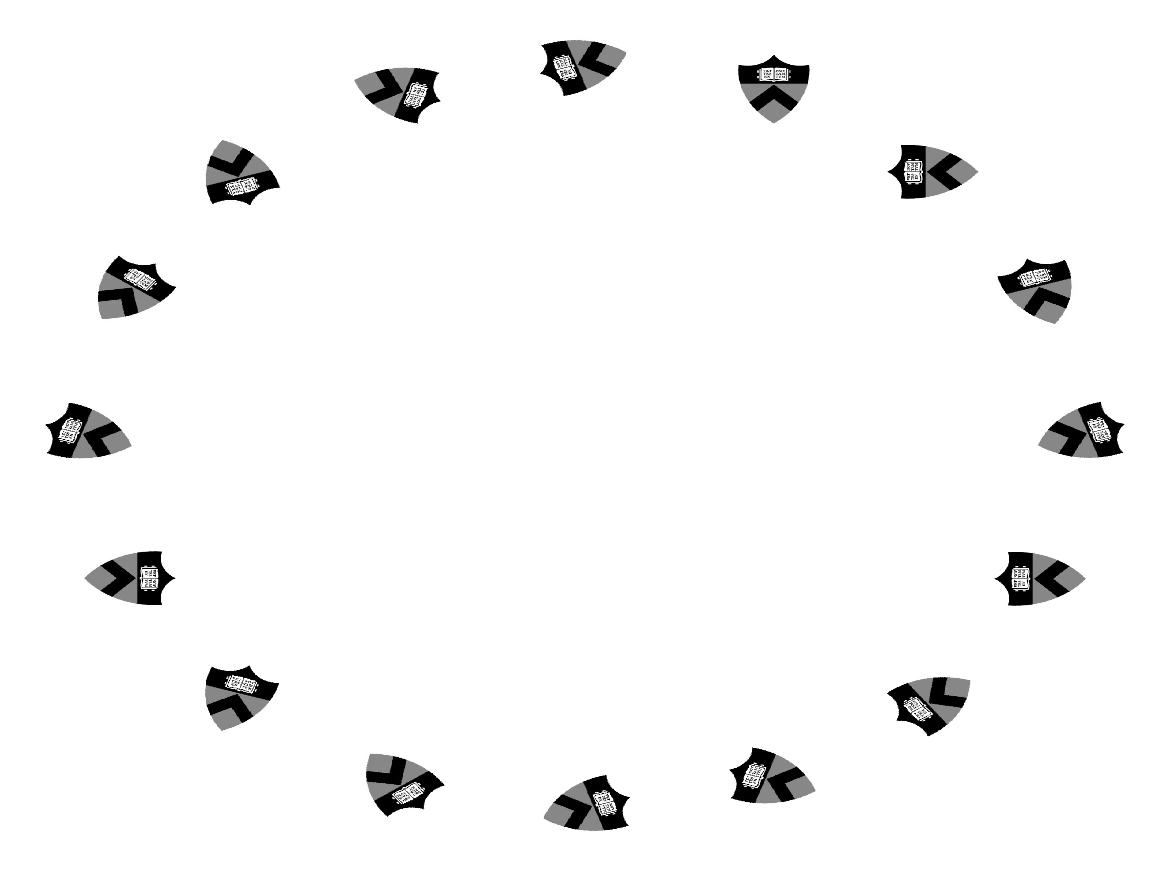
\includegraphics[width=0.5\textwidth, trim=2in 2in 2in 2in, clip]{PU_clean}}
	\only<2>{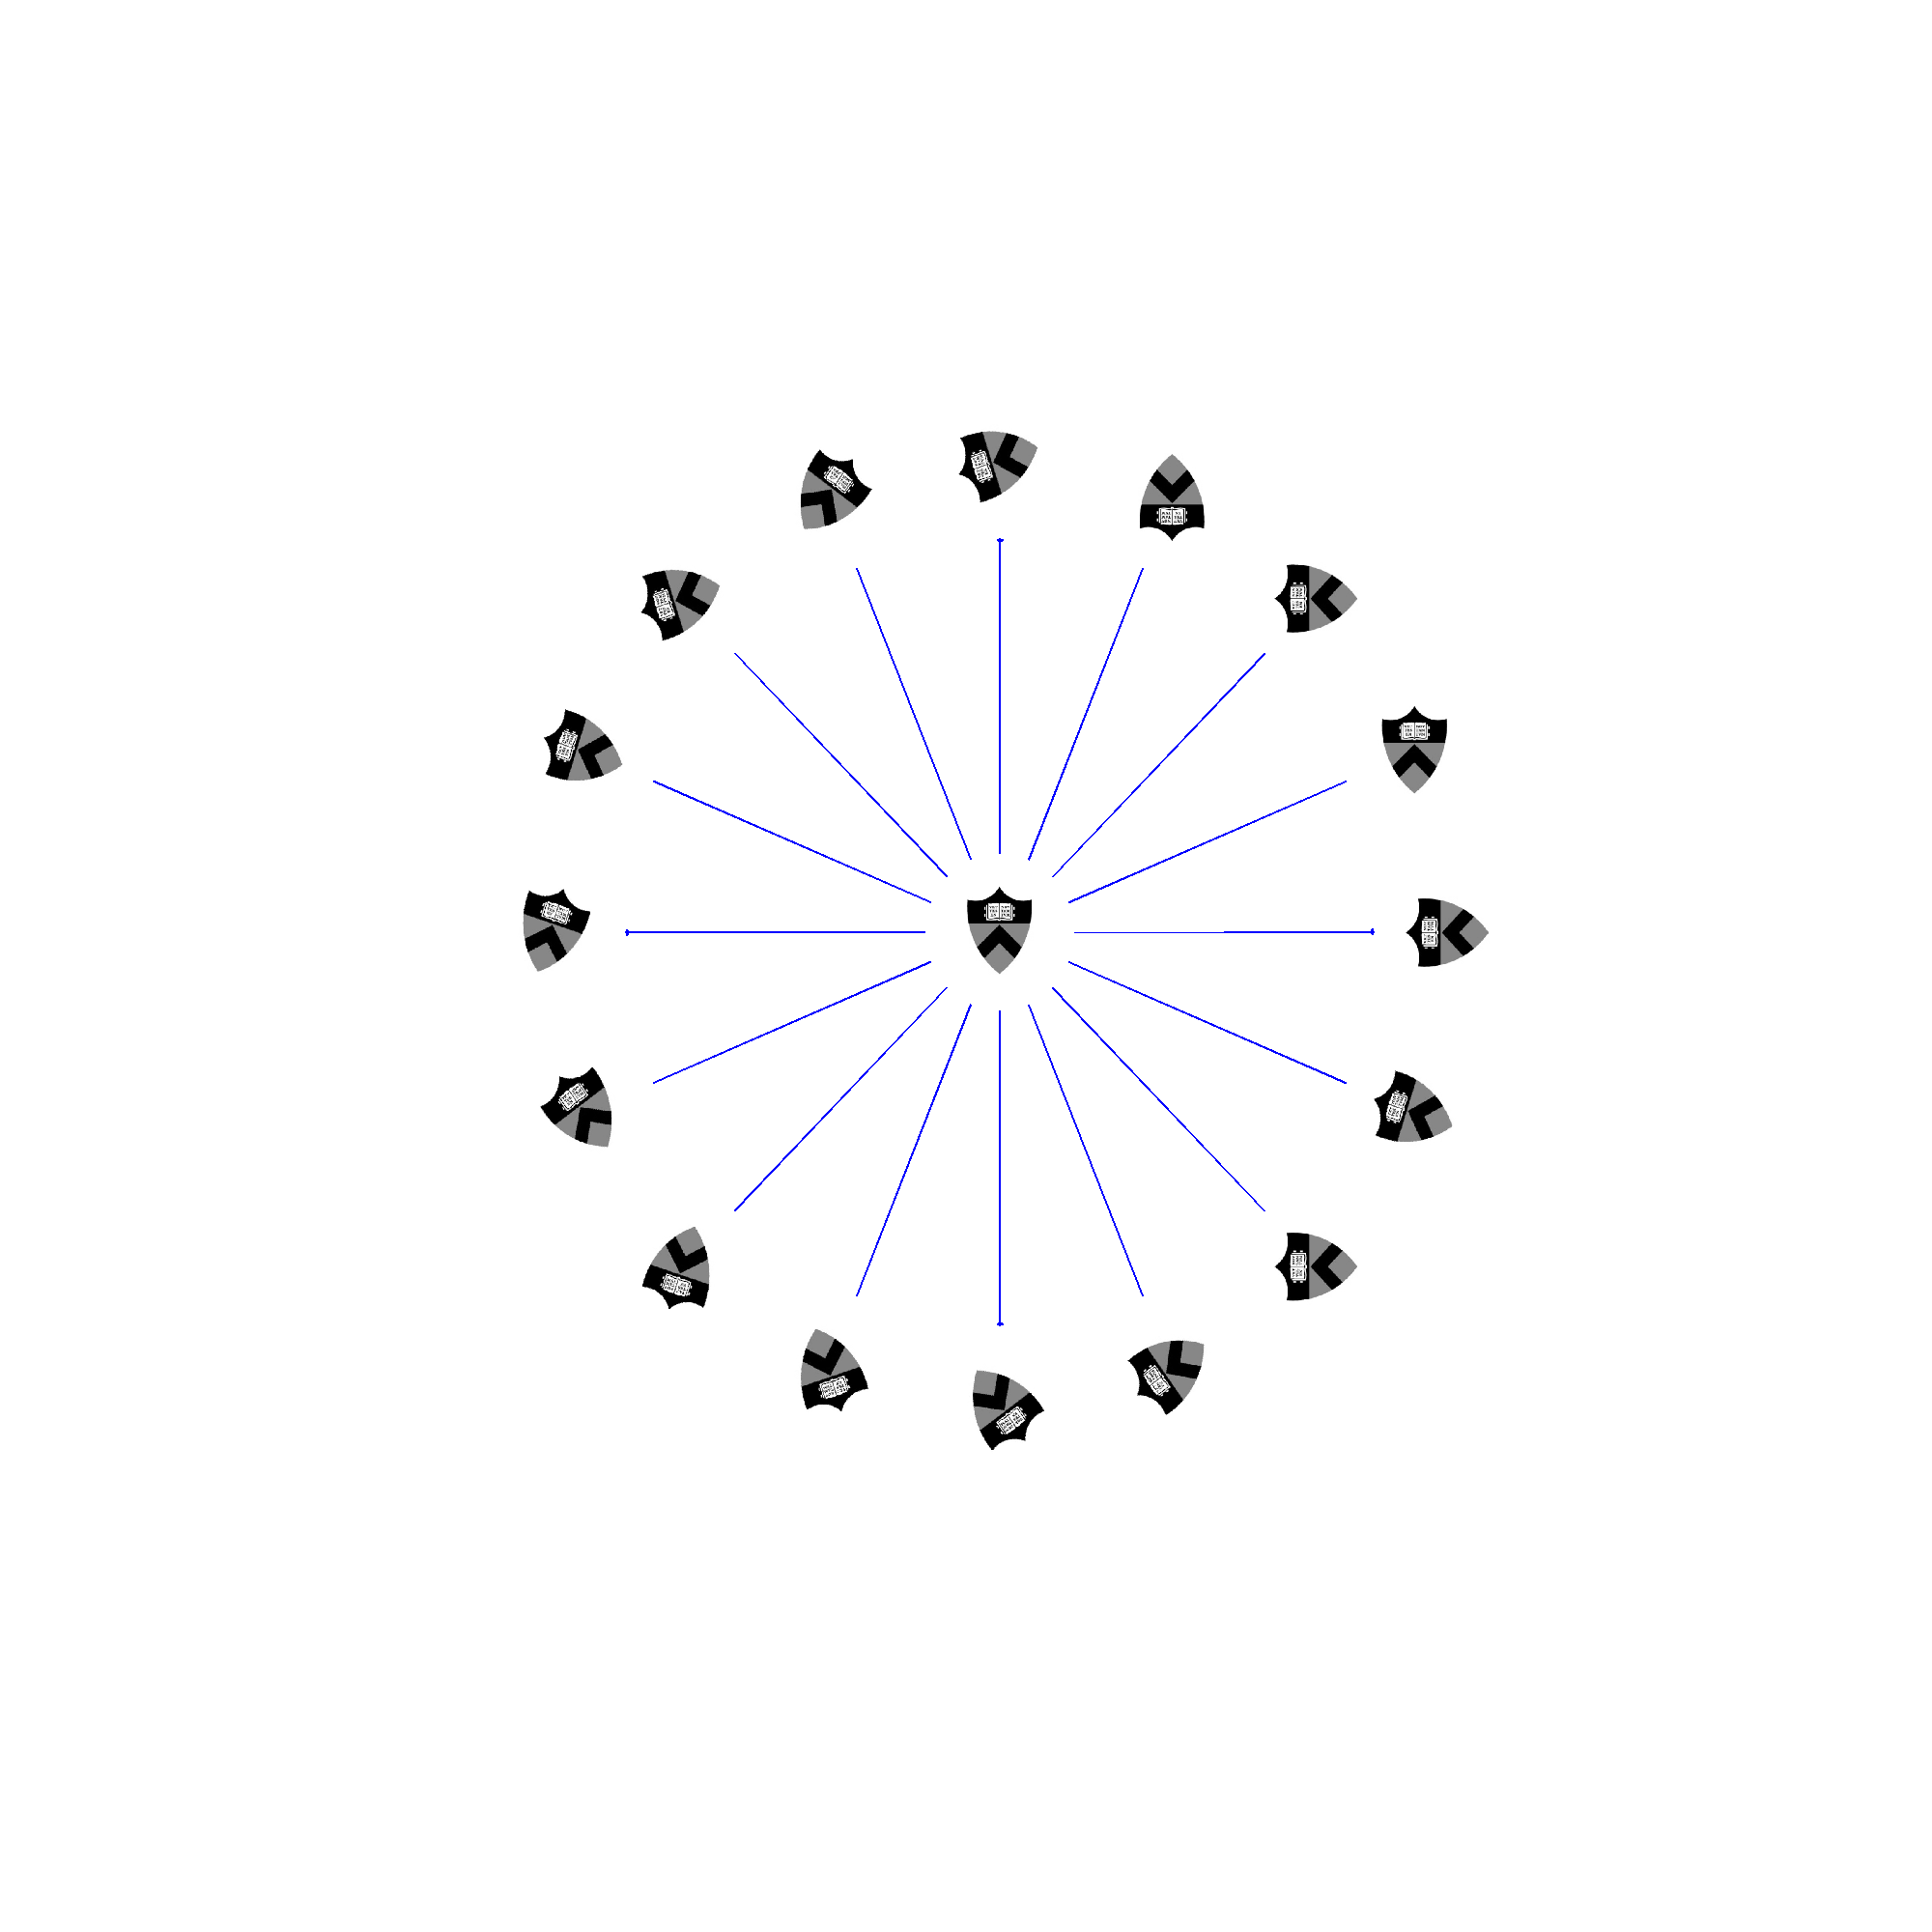
\includegraphics[width=0.5\textwidth, trim=2in 2in 2in 2in, clip]{PU_template1_clean}}
	\only<3>{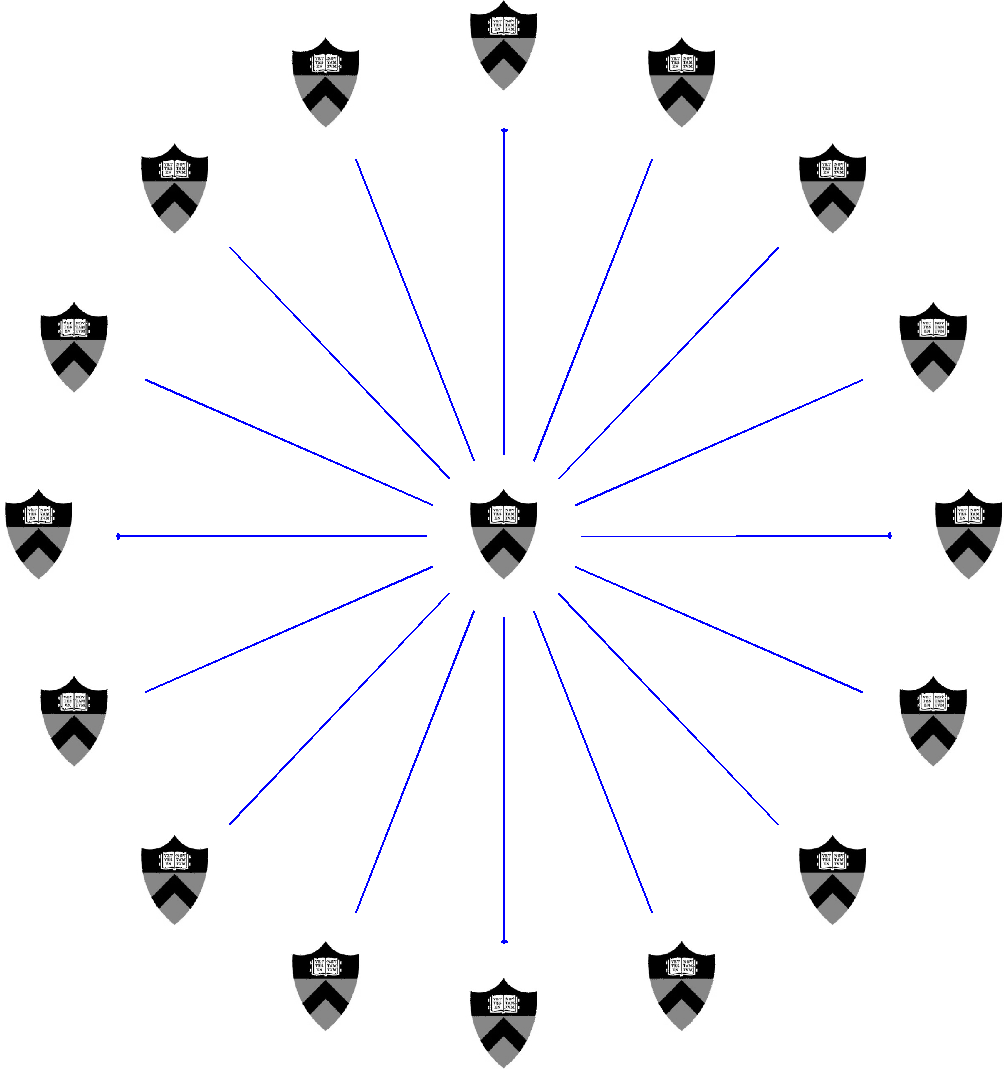
\includegraphics[width=0.5\textwidth, trim=2in 2in 2in 2in, clip]{PU_template2_clean}}

	\only<1>{{\small \em Many images, each of which is a rotated copy of the template.}}
	\only<2>{{\small \em Each image has been rotated to minimize the distance between it and the template.}}
	
	If we have many images and wish to align them, \\ we can rotate each one until it is optimally aligned with a {\bf template}.
	
\end{frame}

\begin{frame}{Factoring Out Rotations}

	\centering
	\only<1>{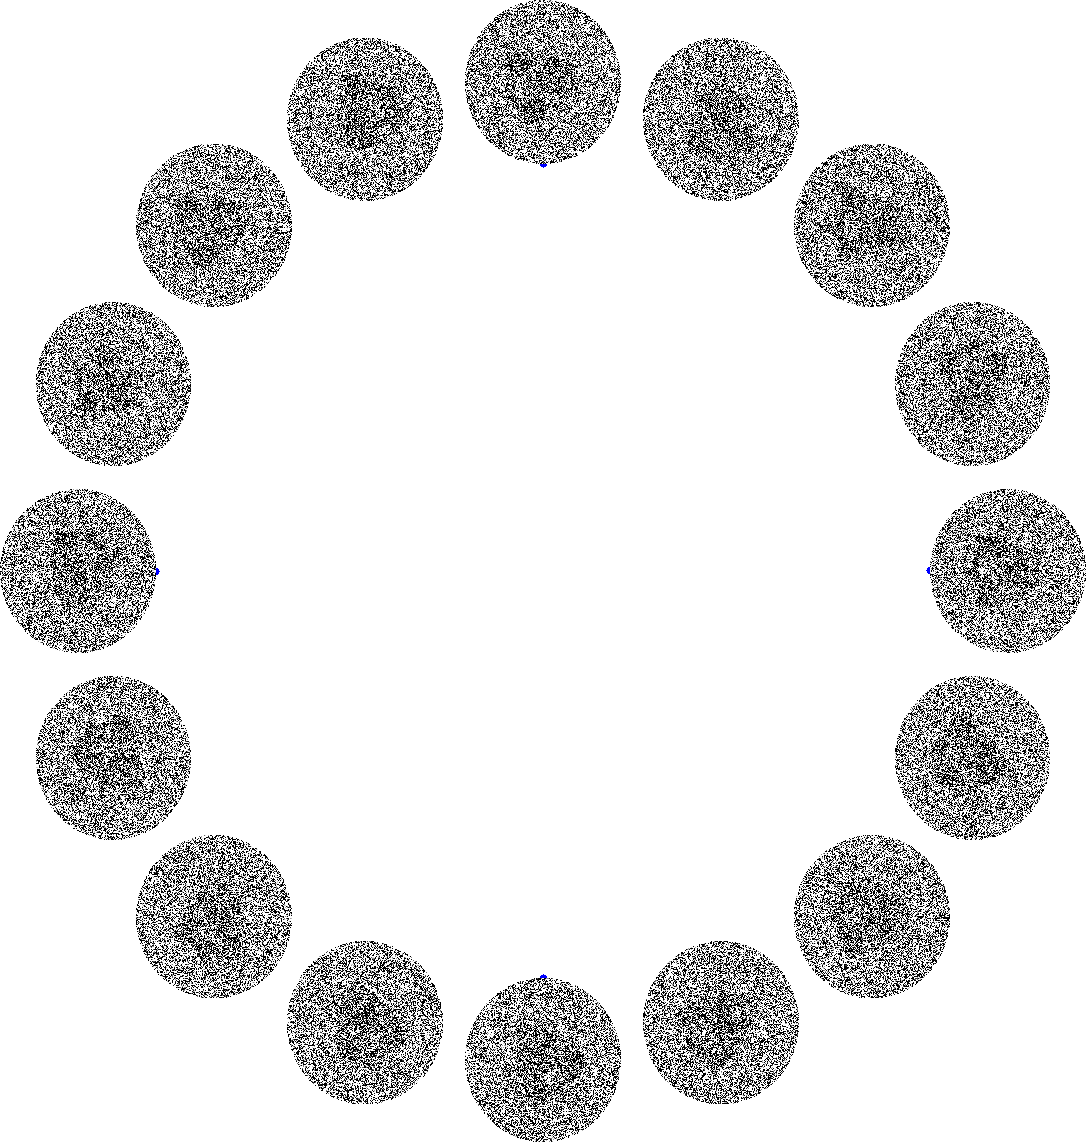
\includegraphics[width=0.5\textwidth]{temp/PU_noisy}}
	\only<2>{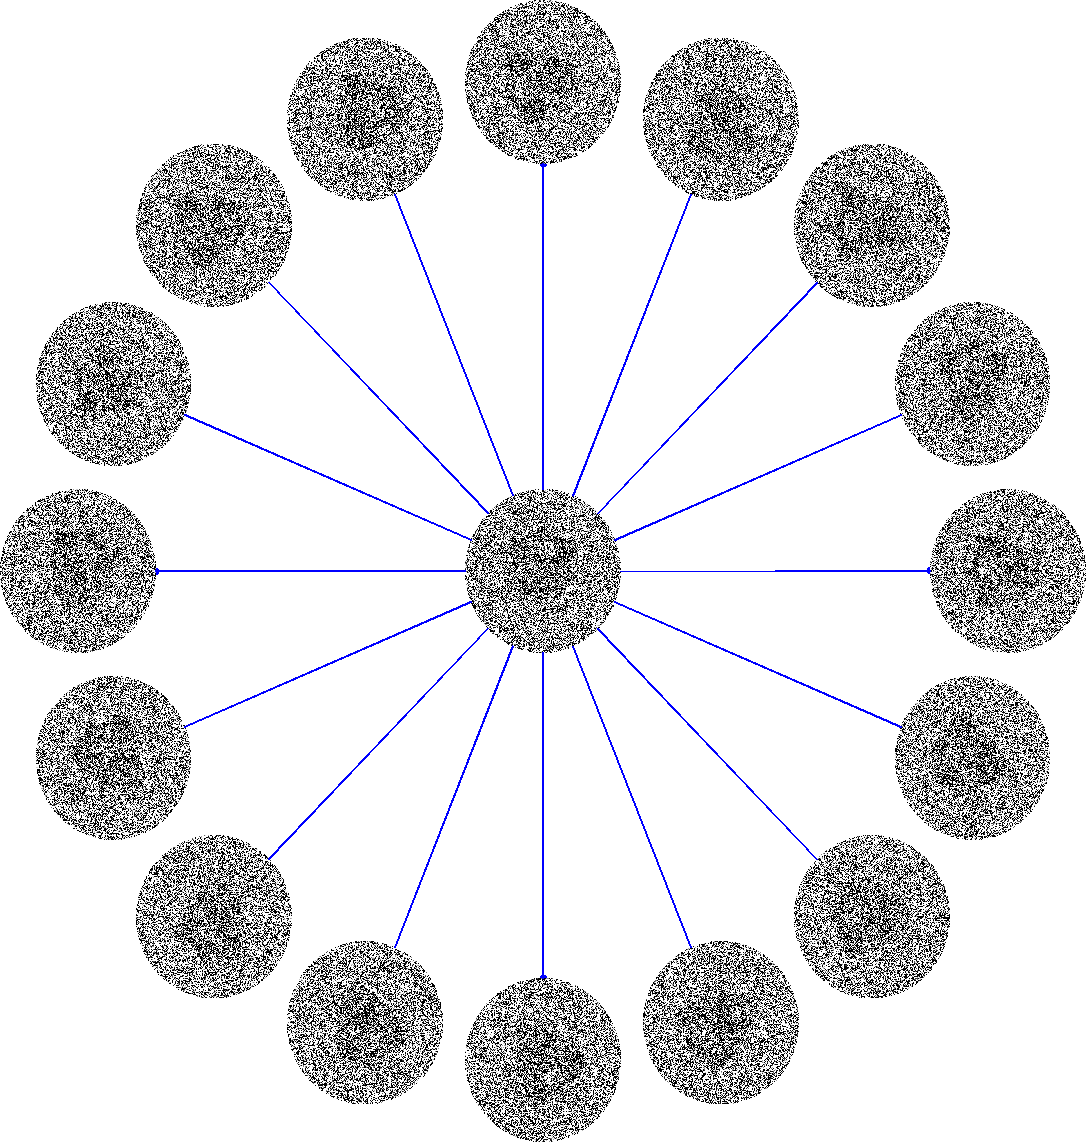
\includegraphics[width=0.5\textwidth]{temp/PU_template1_noisy}}
	\only<3>{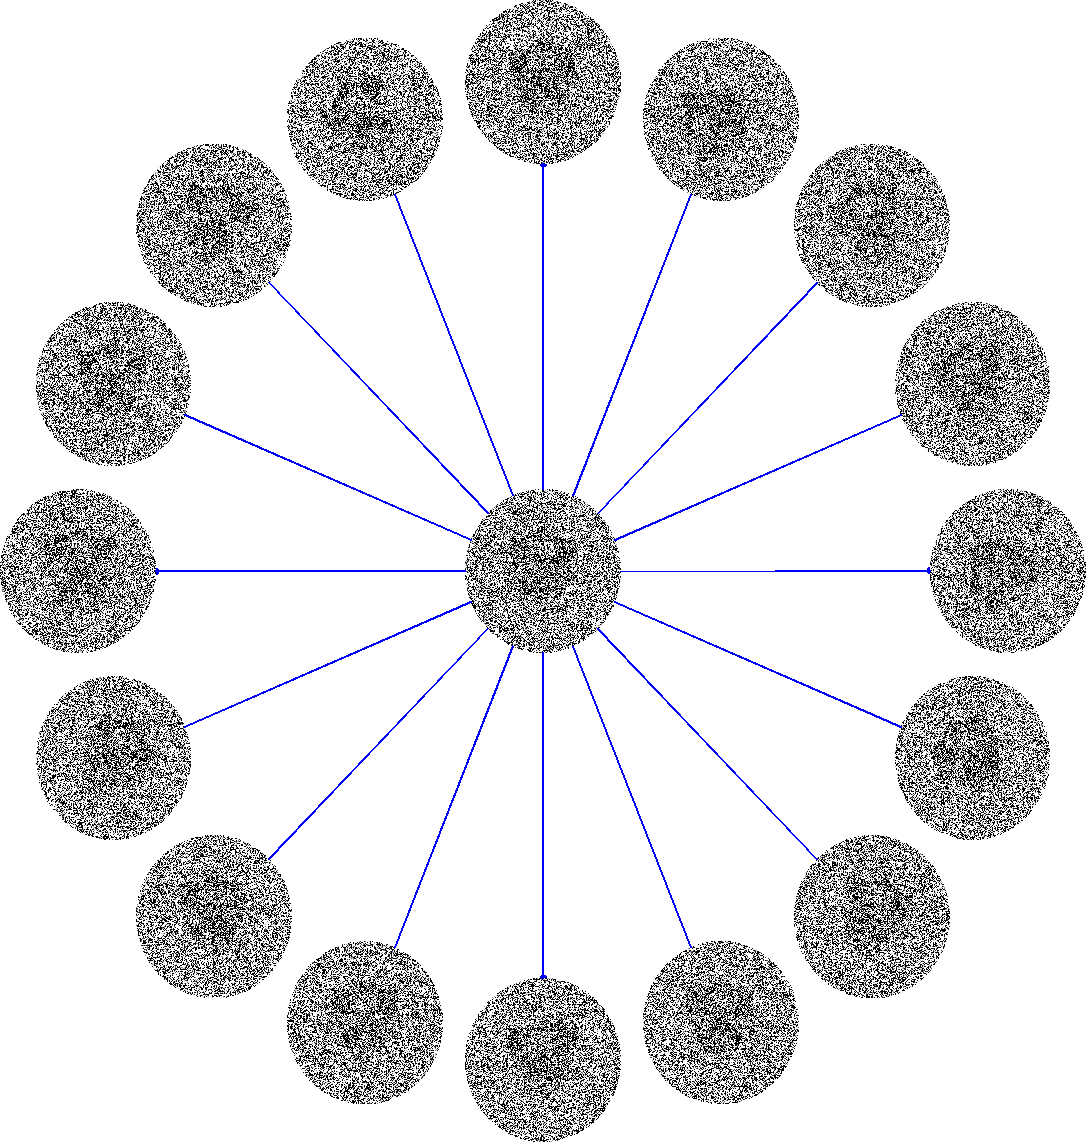
\includegraphics[width=0.5\textwidth]{temp/PU_template2_noisy}}
	\only<4>{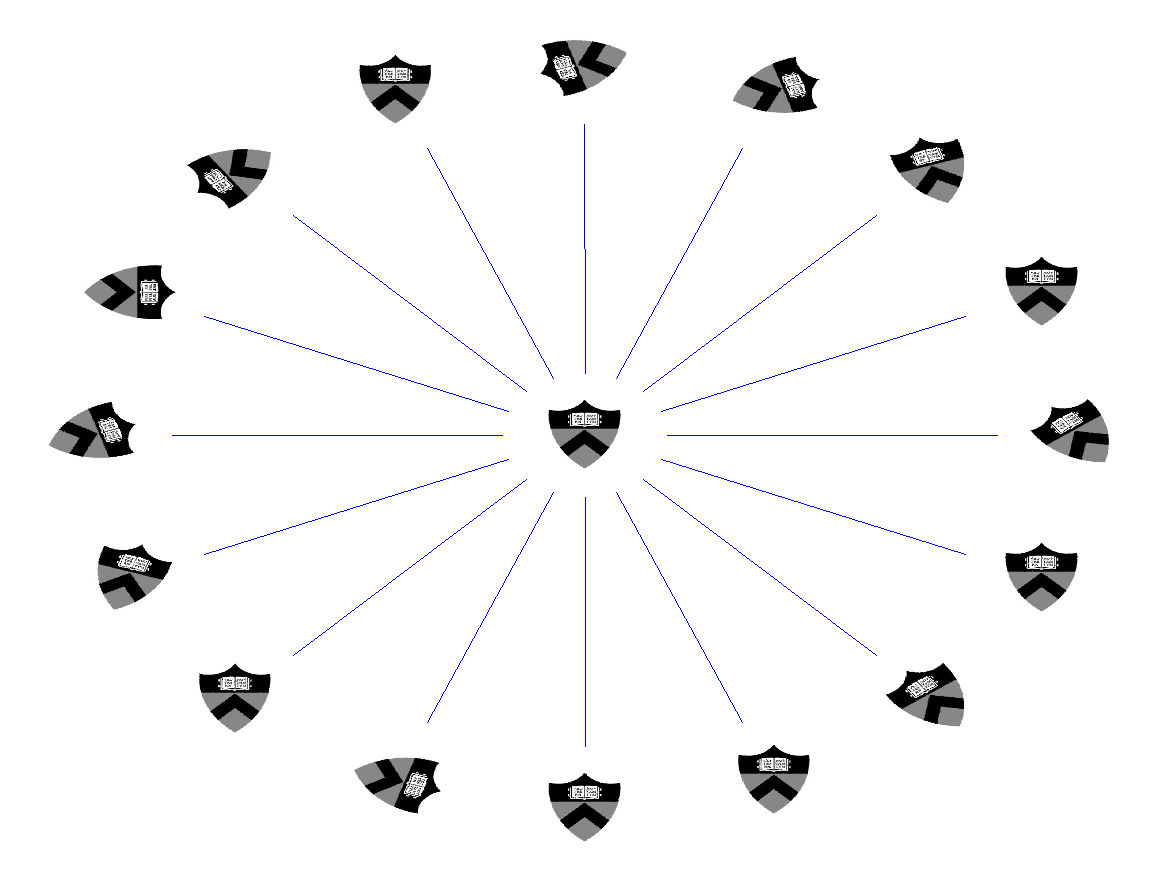
\includegraphics[width=0.5\textwidth]{temp/PU_template3_noisy}}
	
	
	\only<1>{{\small \em Many images, each of which is a rotated noisy copy of the template.}}
	\only<2>{{\small \em Each image has been rotated to minimize the distance between it and the template.}}
	\only<3>{{\small \em There are some misalignments because the images are noisy.}}
	
	However, if the images are noisy, \\then template-based alignment will often be inaccurate.
	
\end{frame}

\begin{frame}{Factoring Out Rotations}
	
	Instead, we would like to use each image as a template for every other image, and then find the most {\em consistent} set of alignments.
	
	\centering
	\only<1>{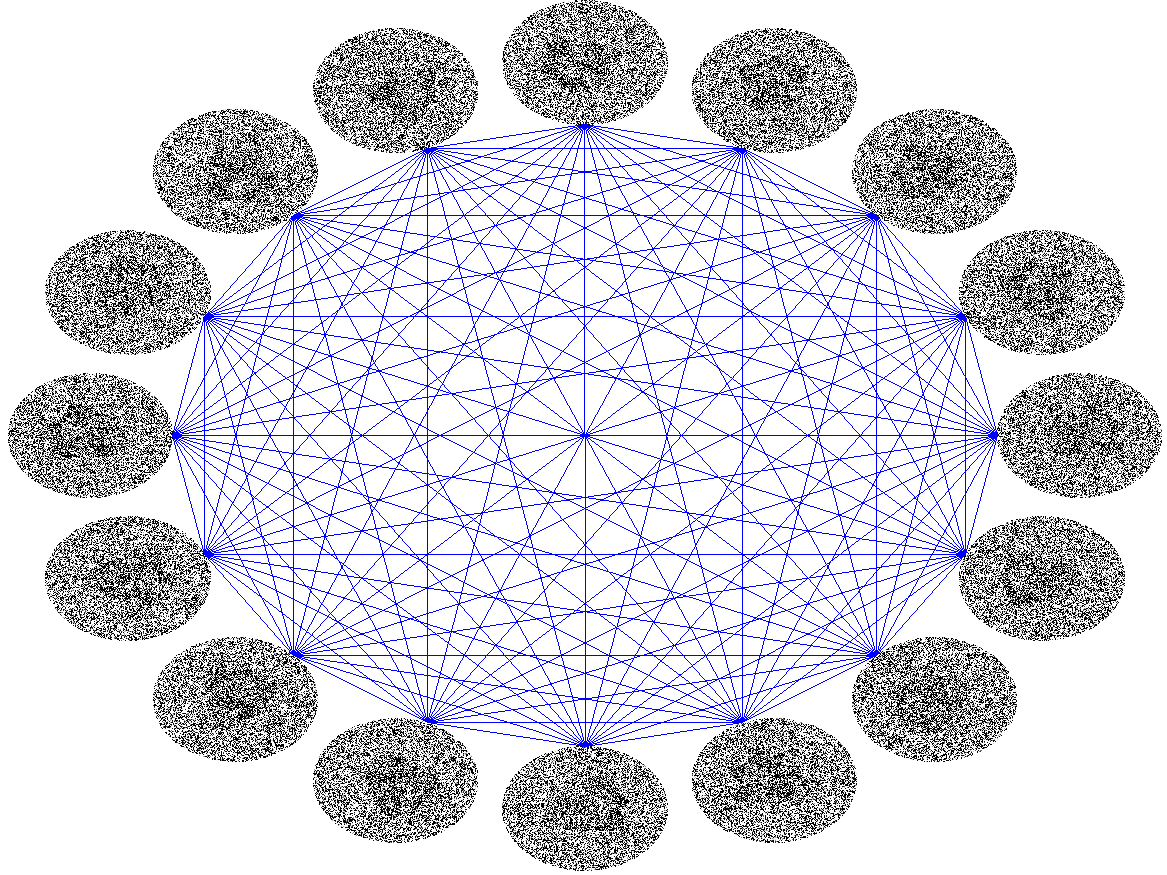
\includegraphics[width=0.5\textwidth]{PU_angsynch1}}
	\only<2>{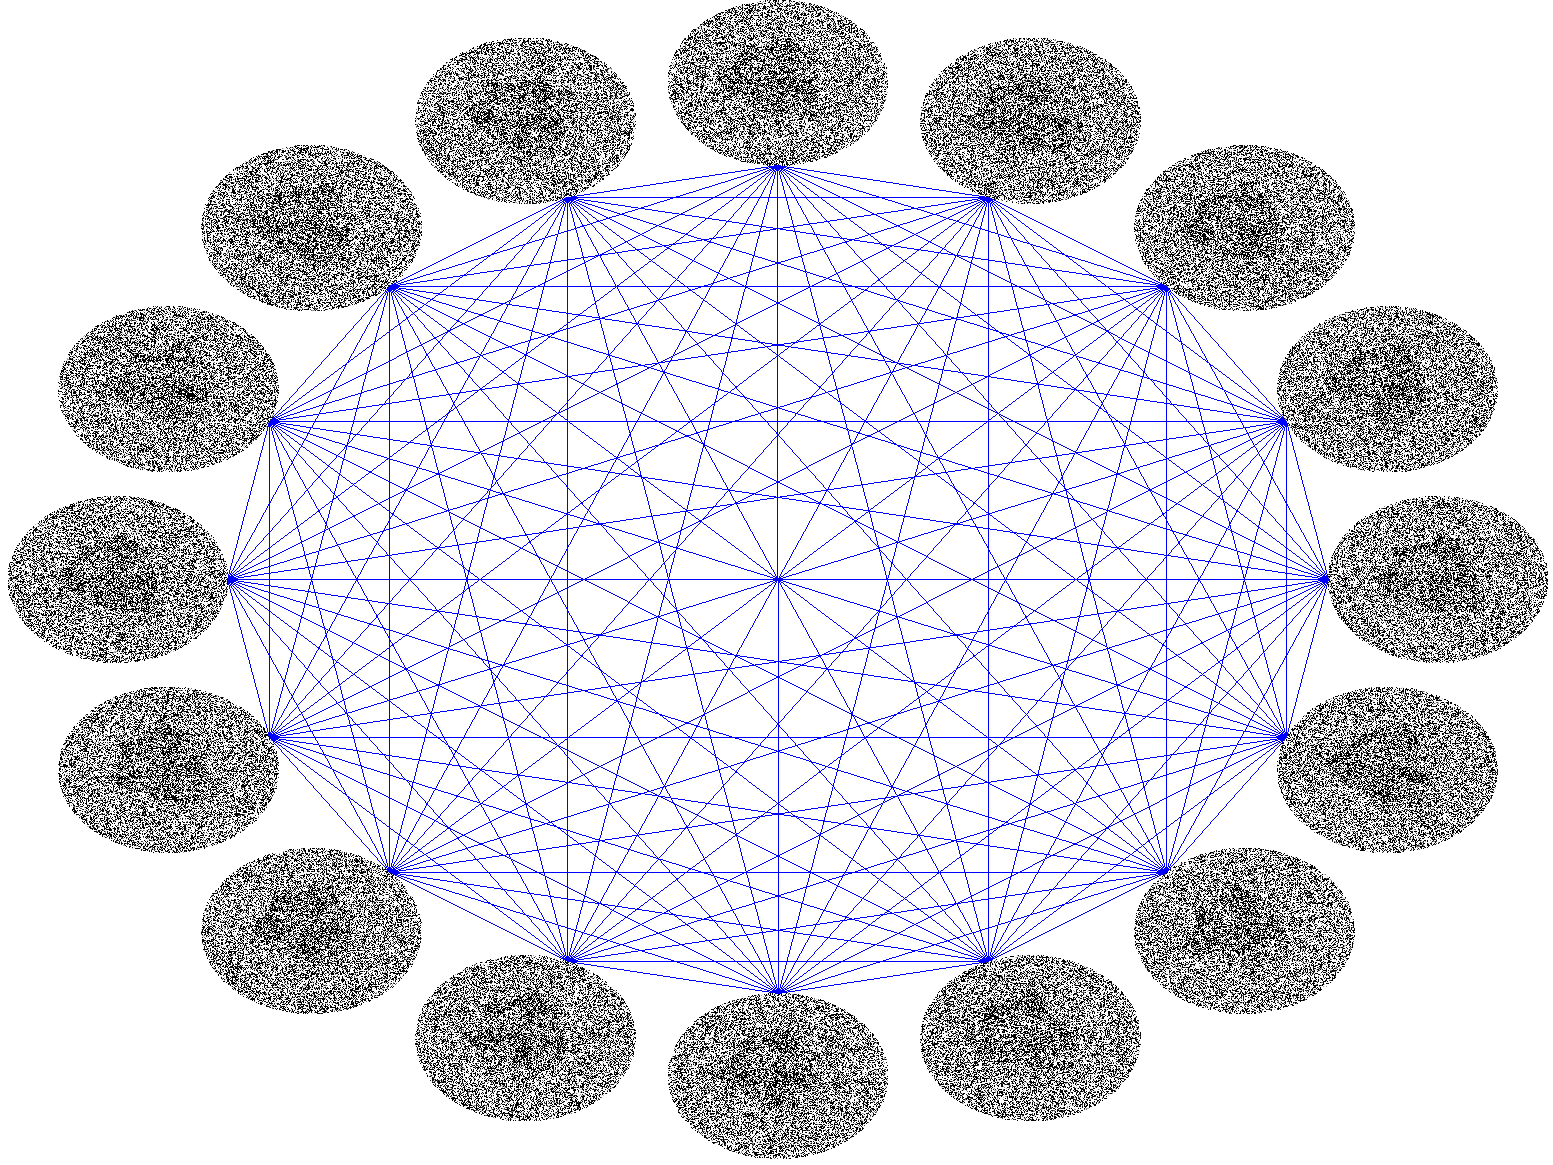
\includegraphics[width=0.5\textwidth, trim=2in 2in 2in 2in, clip]{PU_angsynch2}}
	\only<3>{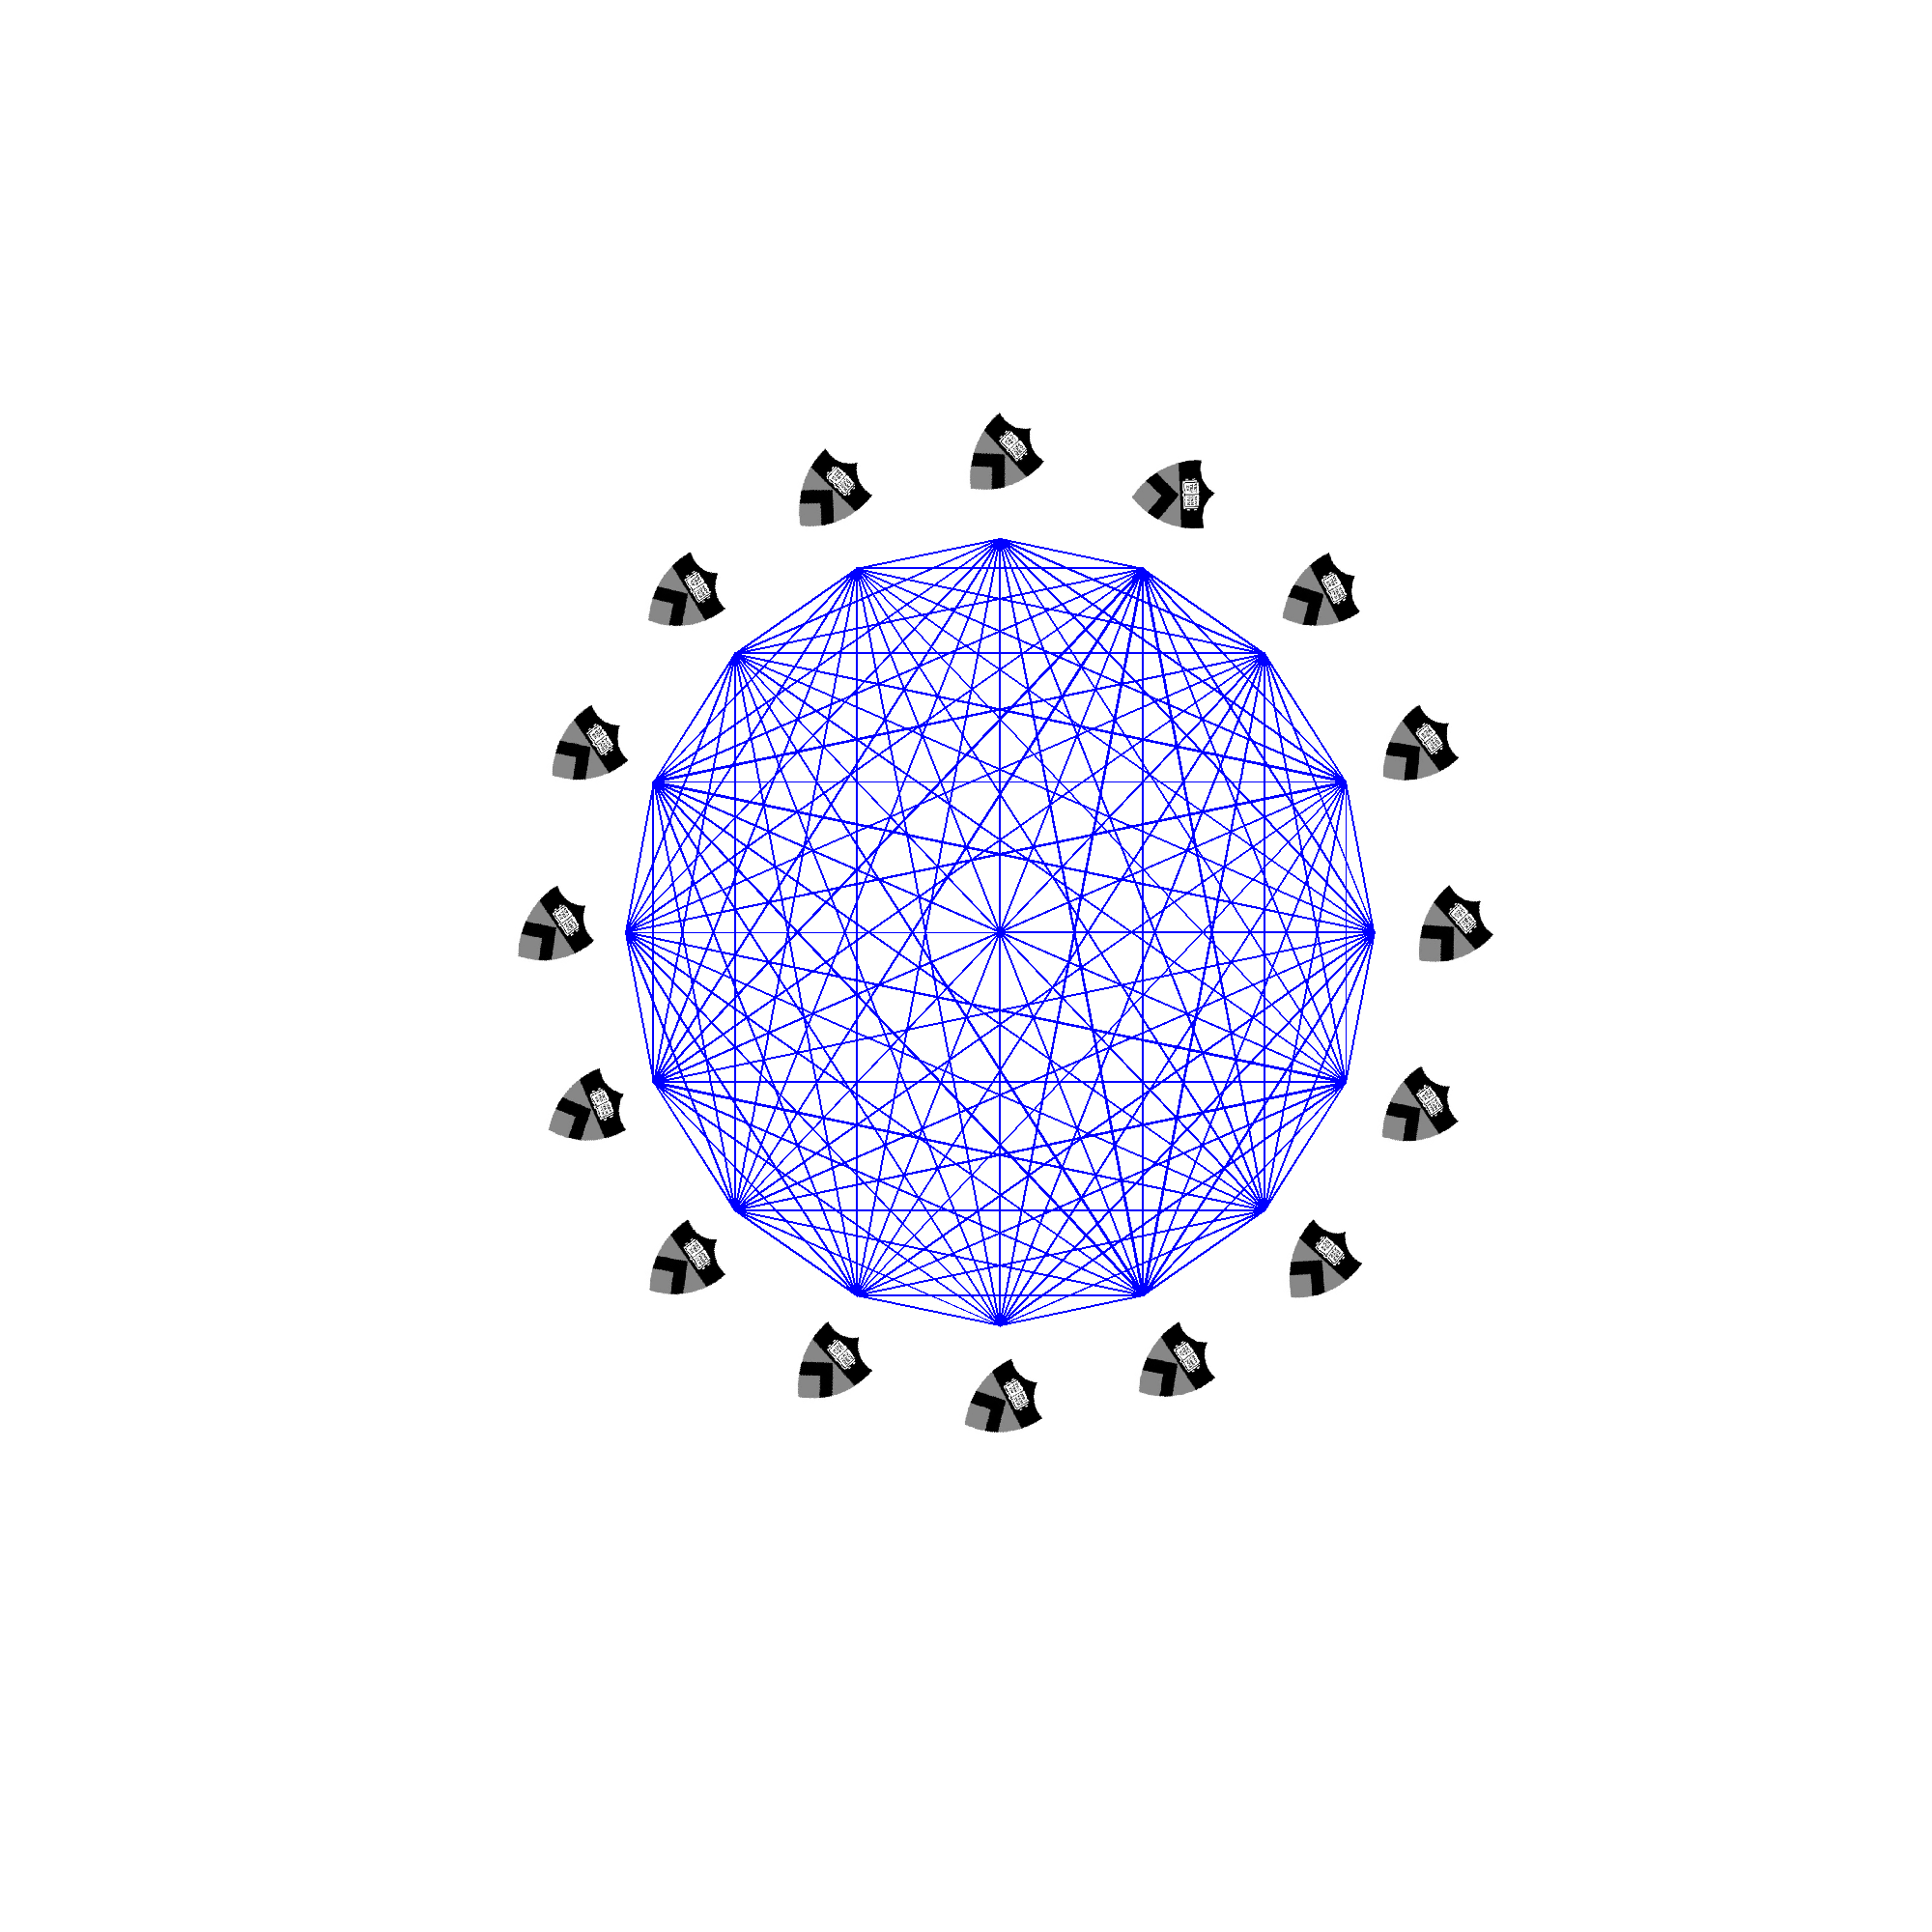
\includegraphics[width=0.5\textwidth, trim=2in 2in 2in 2in, clip]{PU_angsynch3}}
	
\end{frame}

\begin{frame}{Angular Synchronization for Data Alignment}

	\begin{block}{Angular Synchronization Algorithm \footnotemark}
		{\scriptsize 
		 We have {\bf data} $x_1, x_2, \dots, x_n$ (e.g., $x_i$ is the concentration profile of dpERK on a ring).
        
        $\theta_{ij}$ denotes the {\bf angle of rotation} that best aligns $x_i$ and $x_j$.

        We {\bf construct the matrix} $H$, where $H_{ij} = e^{i \theta_{ij}}$.

		The entries of $v_1$, the {\bf top eigenvector} of $H$, contain estimates of the optimal rotations for each data point.

		The optimal rotations $\hat{\theta_1}, \dots, \hat{\theta_n}$ are given by $e^{i \hat{\theta_i}} = \frac{v_1(i)}{|v_1(i)|}$.
		\par}
	\end{block}	
	\footcitetext{singer2011angular}
	
	We can use angular synchronization to align the concentration profiles
	
	\begin{tikzpicture}
		\node[] (fig1) {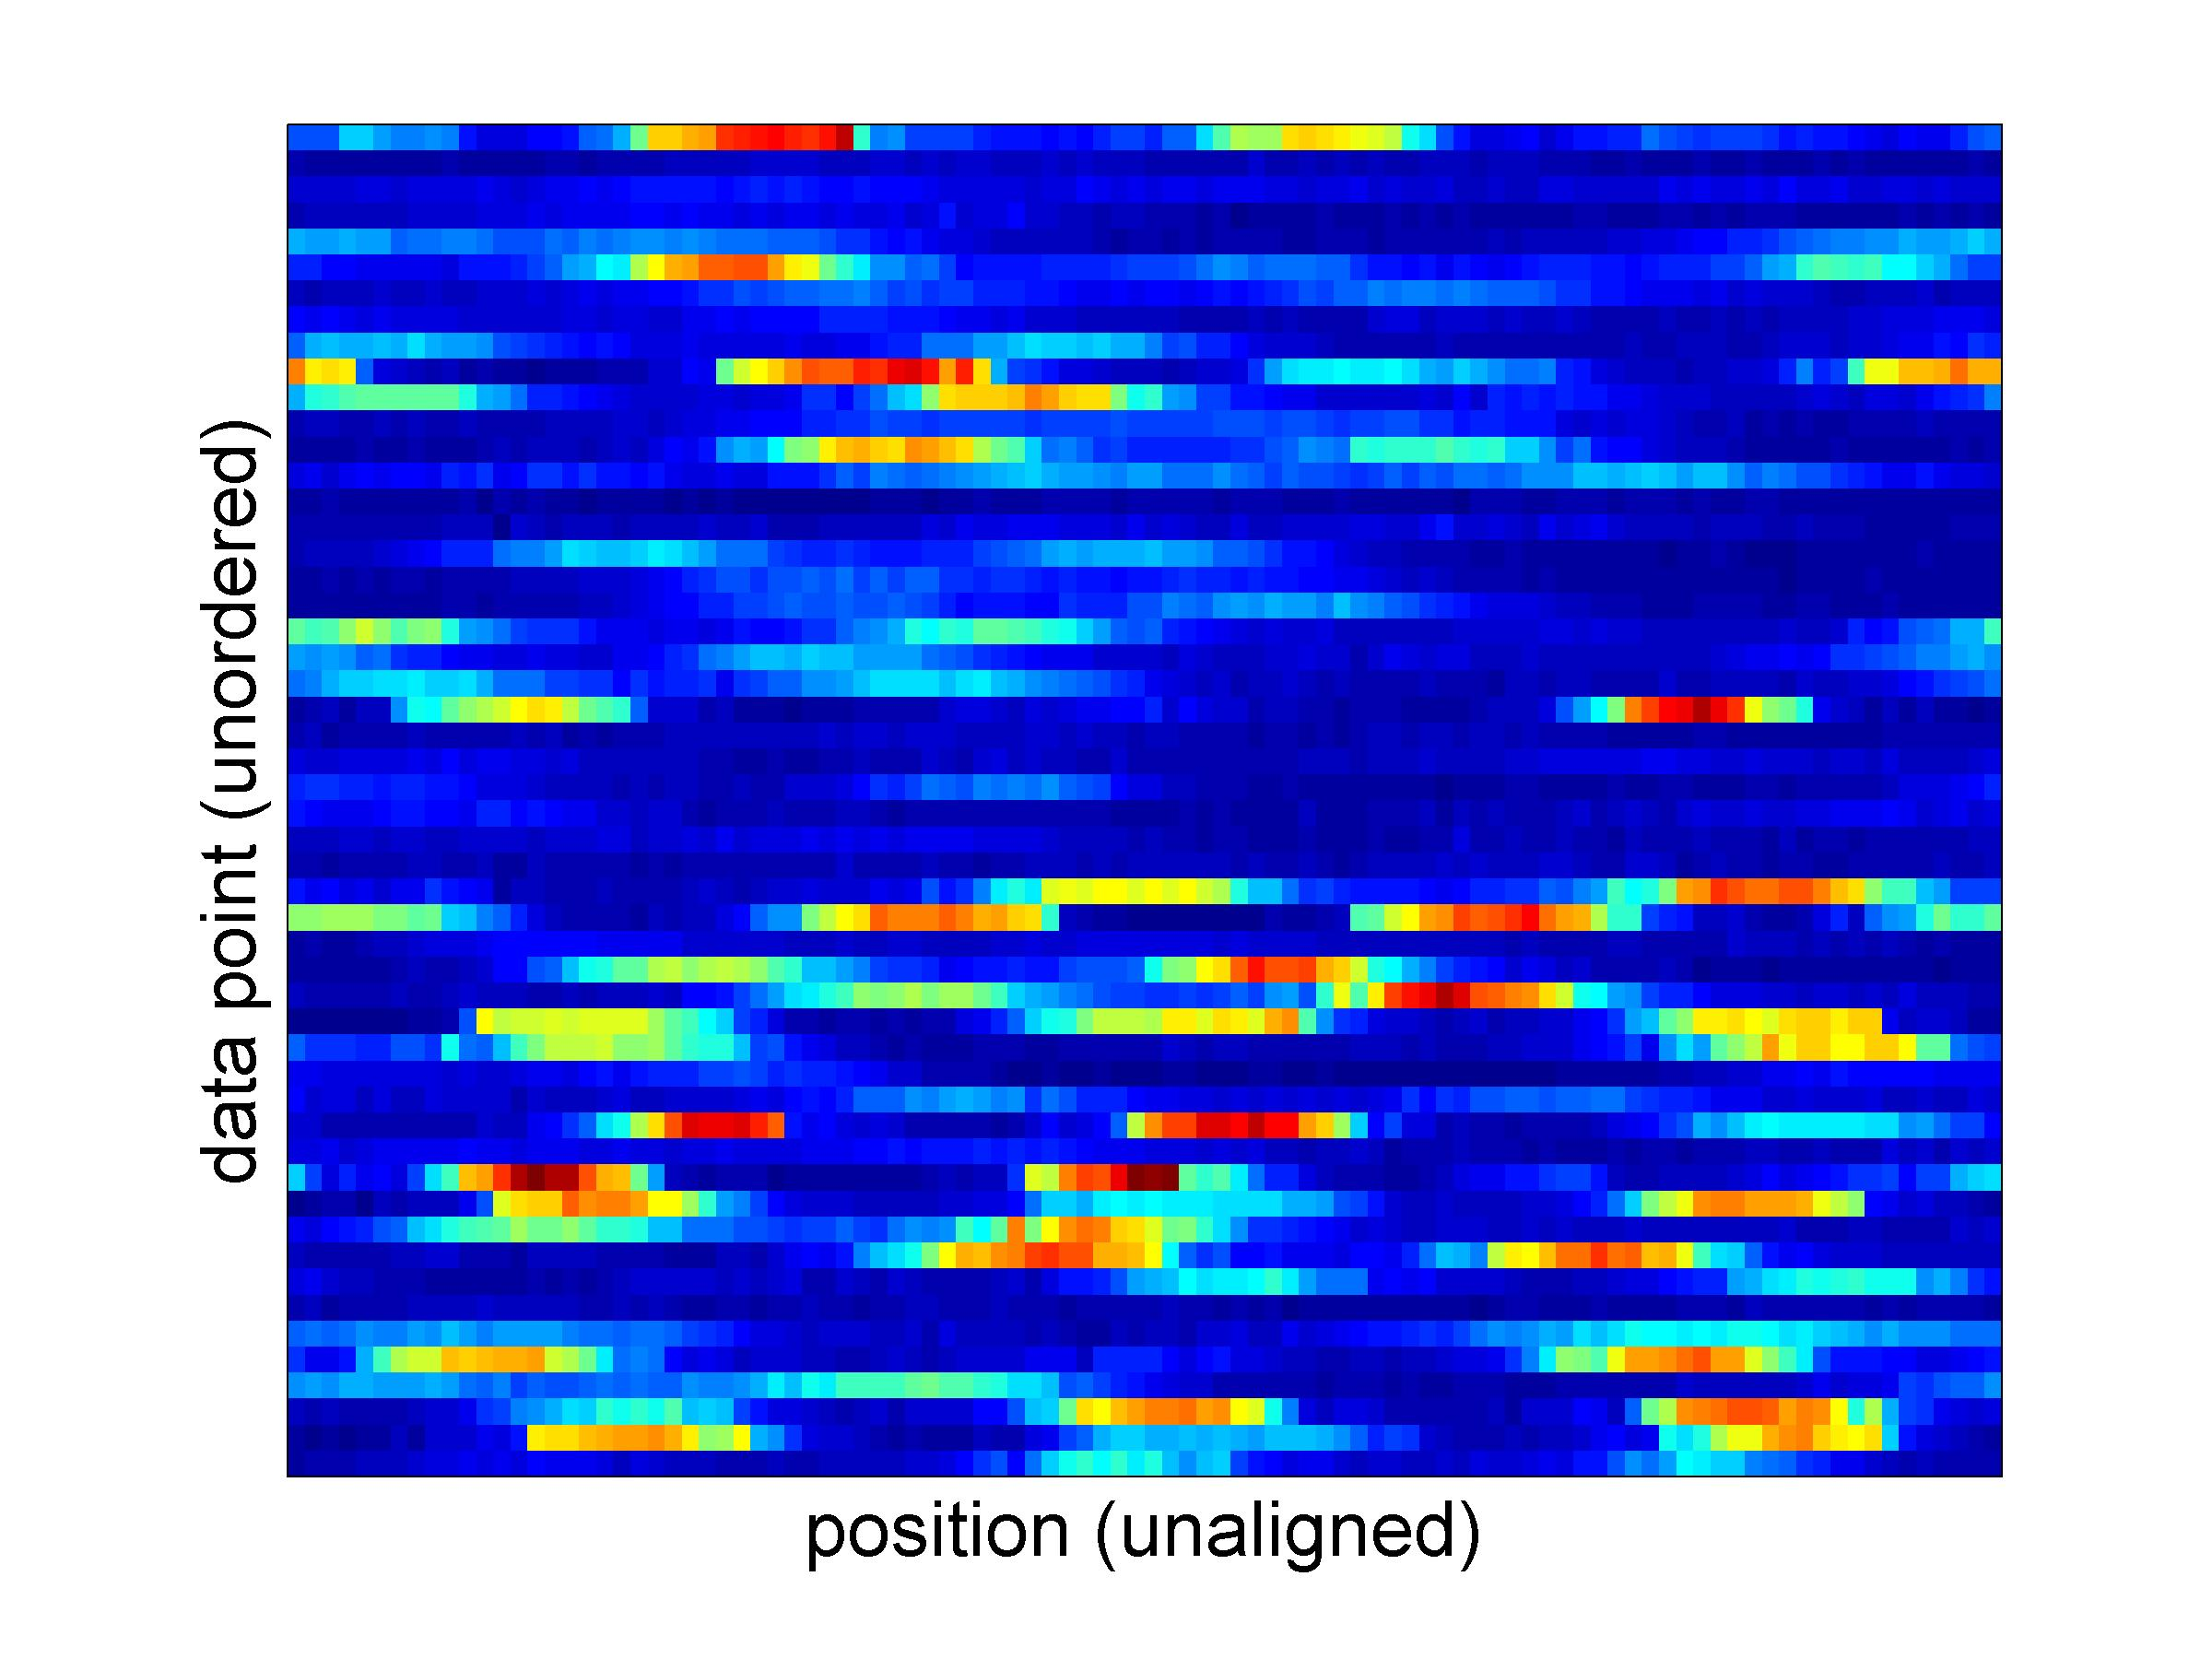
\includegraphics[width=0.25\textwidth]{data_unaligned_unordered}};
		\node[right of=fig1, node distance=0.35\textwidth] (fig2) {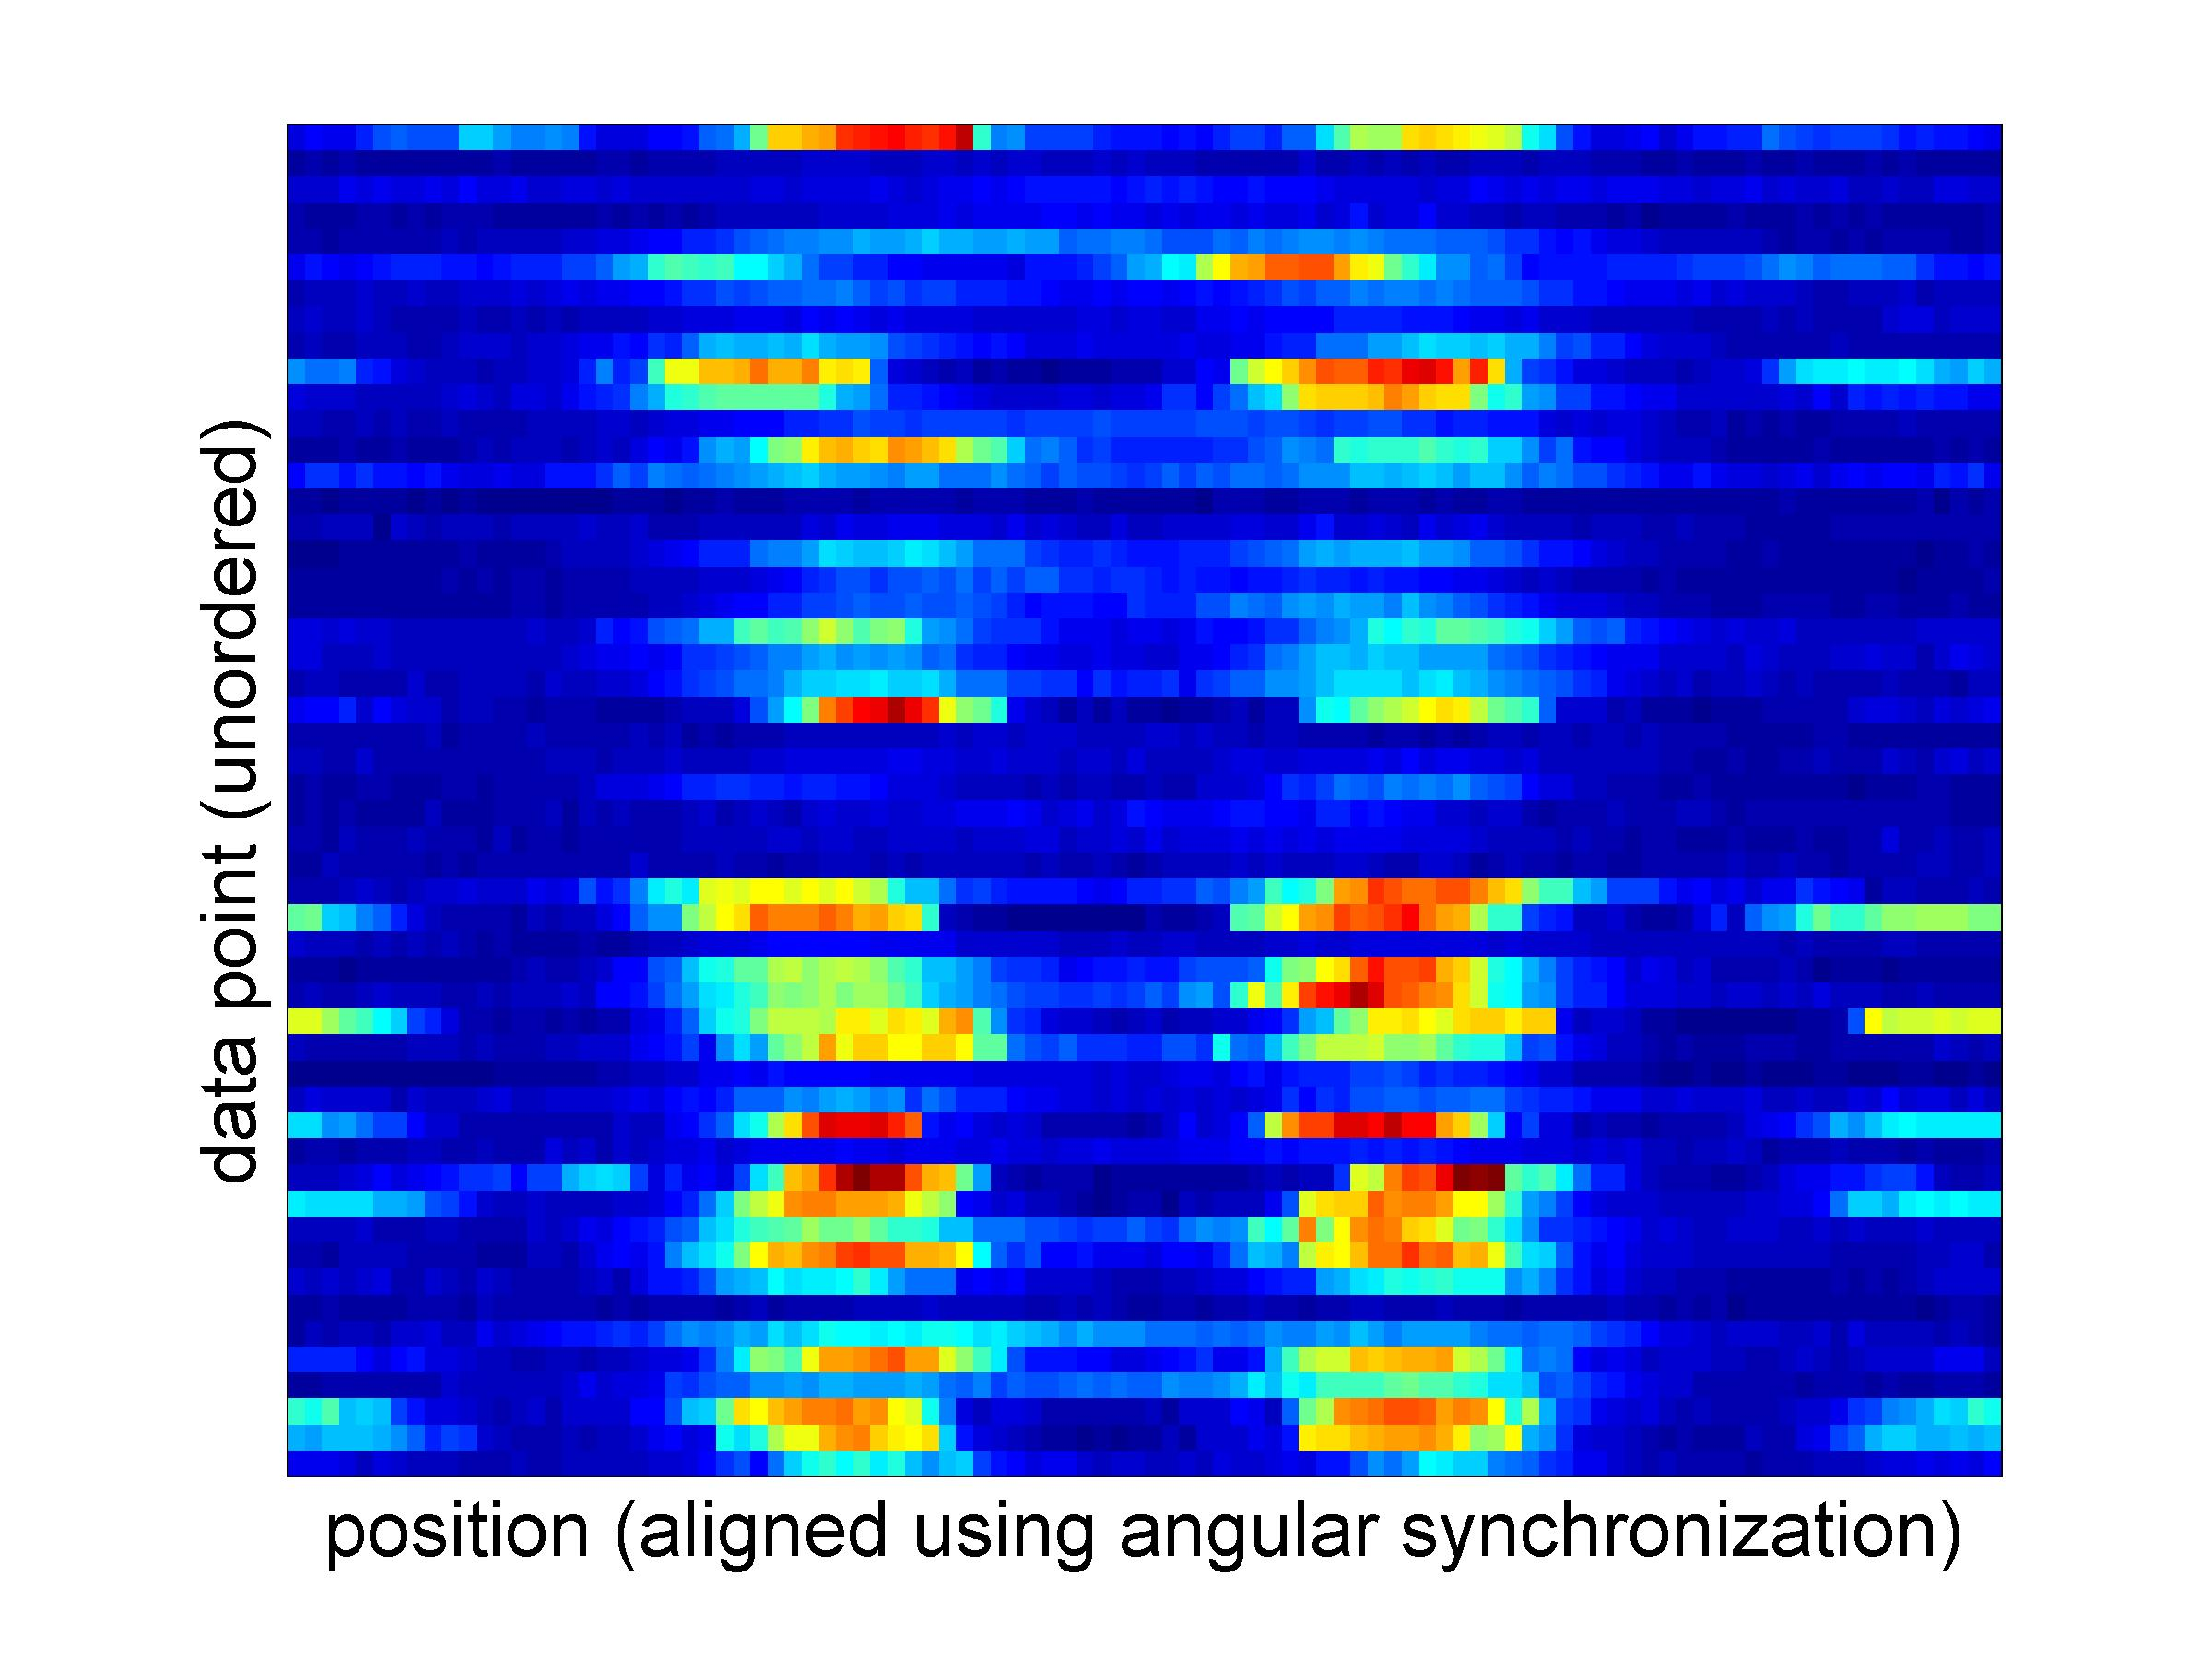
\includegraphics[width=0.25\textwidth]{data_aligned_unordered}};
		\node[right of=fig2, node distance=0.35\textwidth] (fig3) {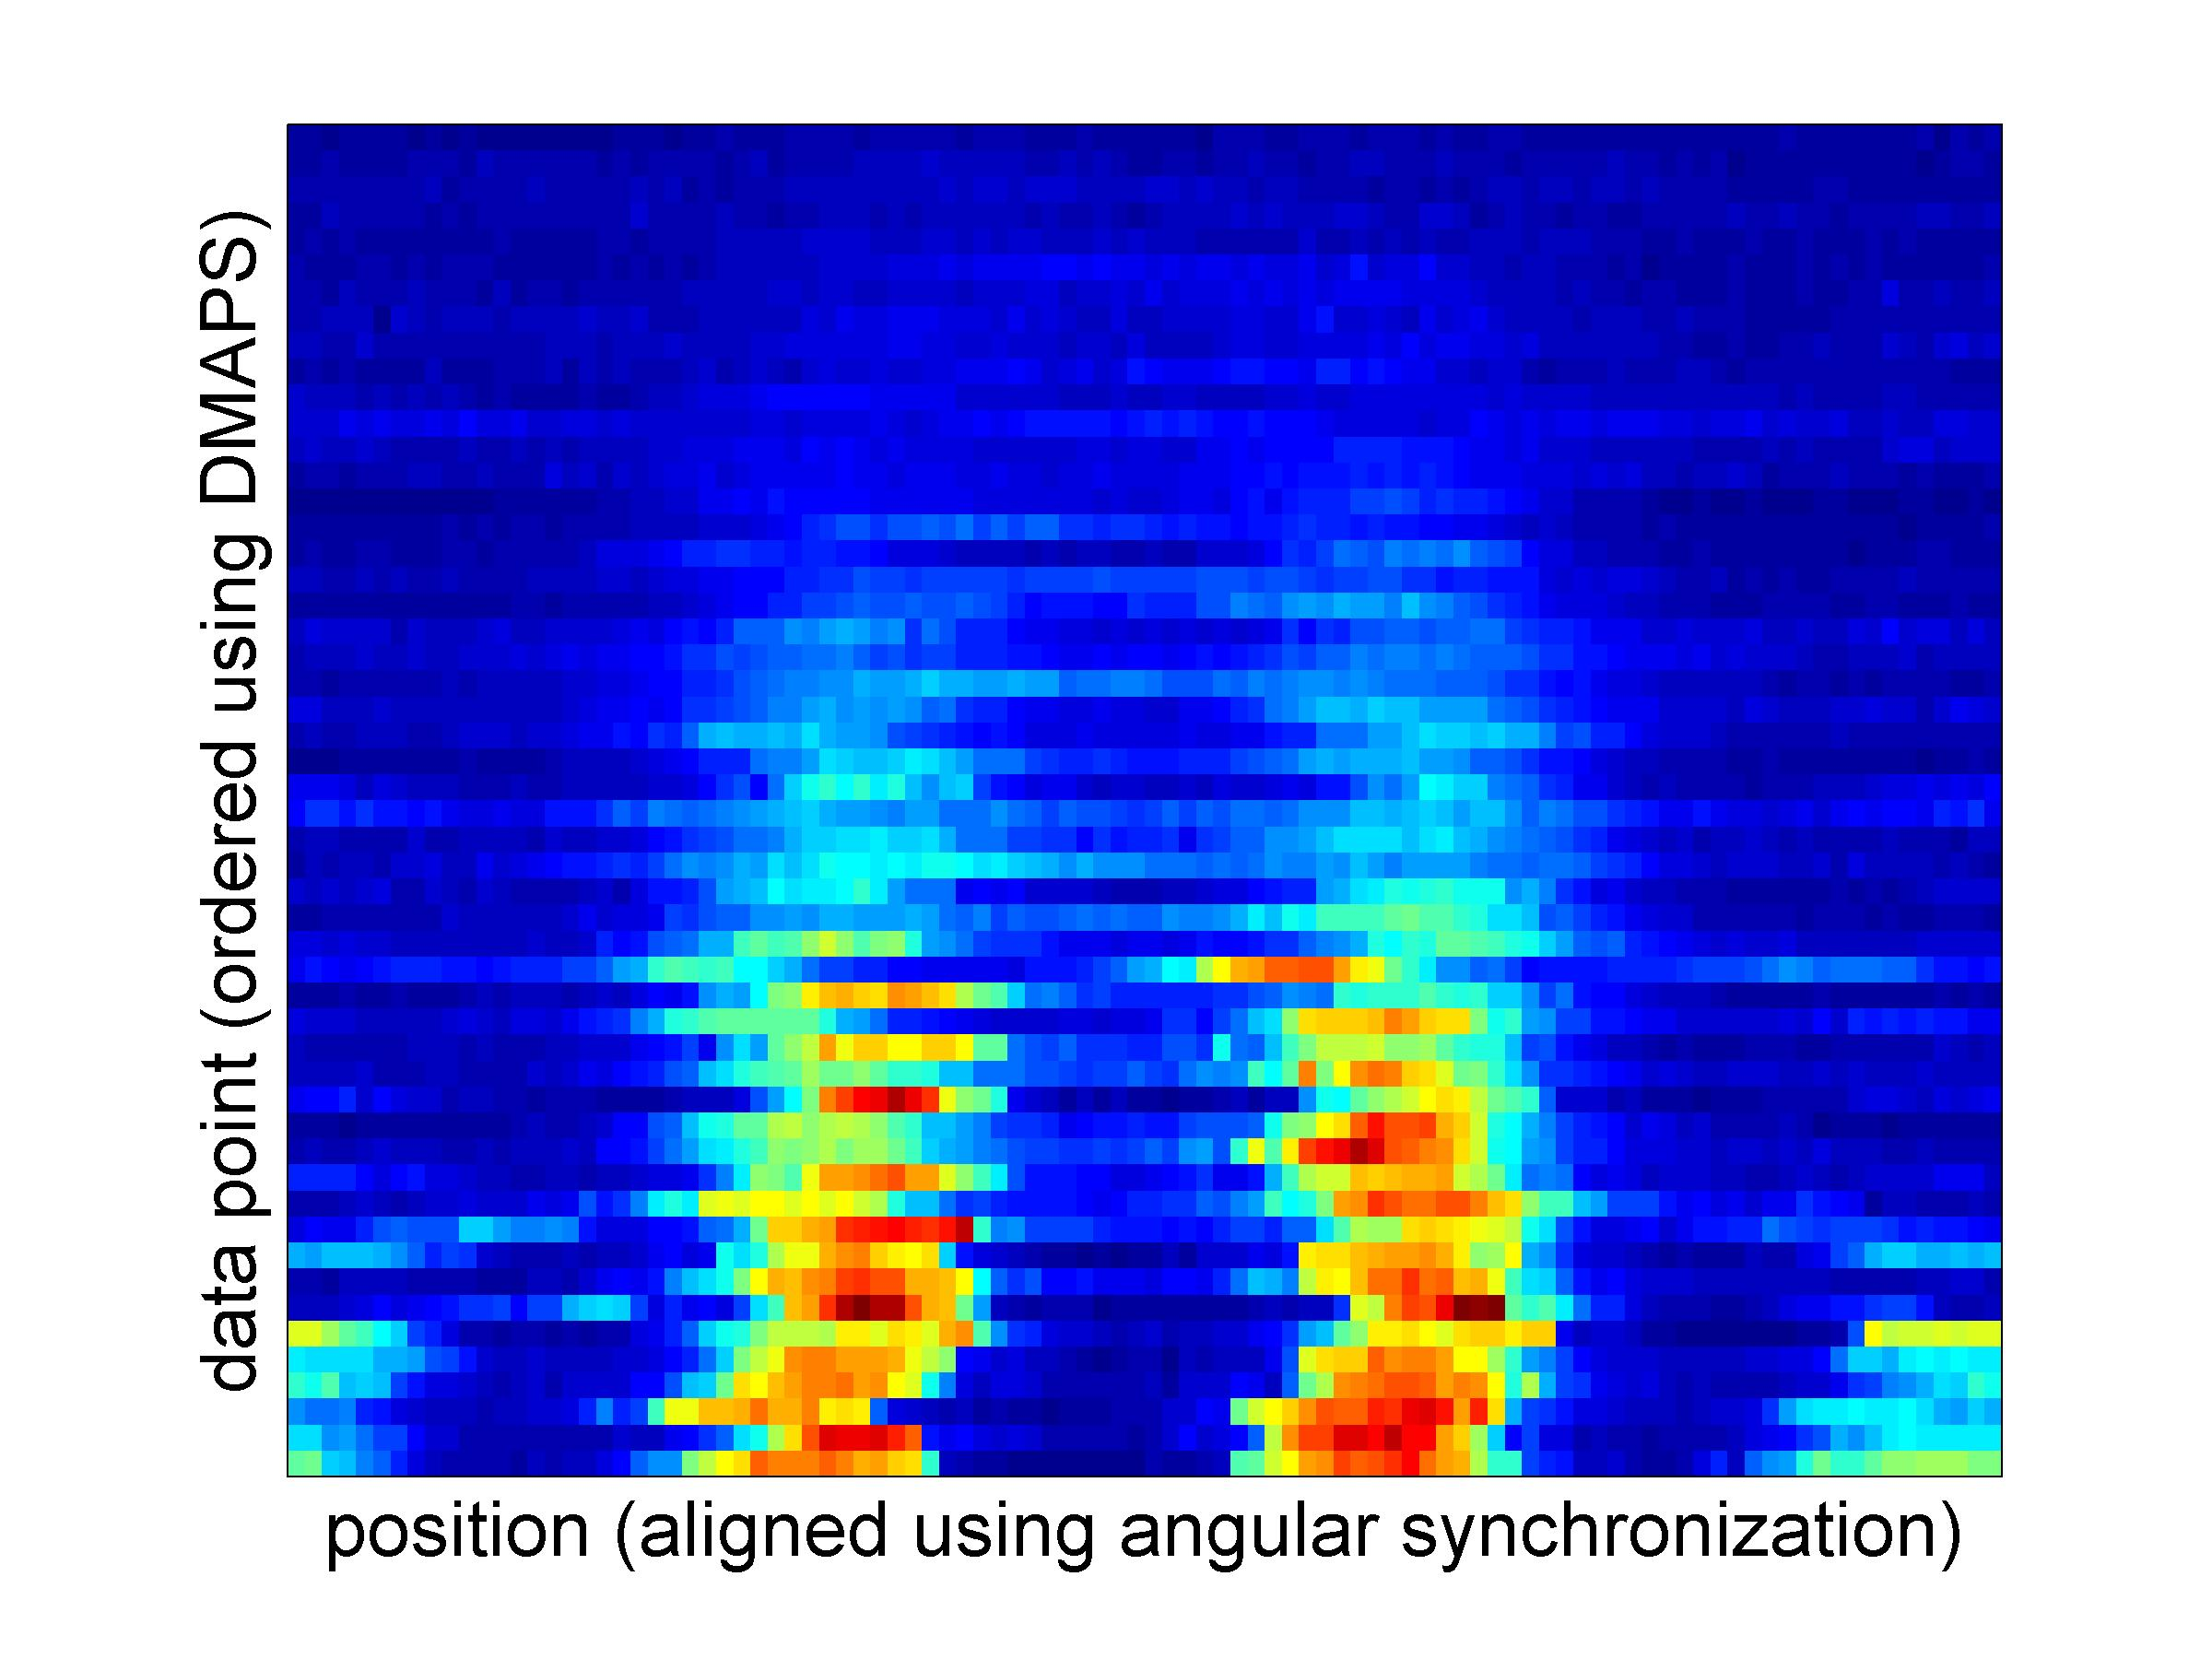
\includegraphics[width=0.25\textwidth]{data_ordered_angsynch}};
		\draw[->] (fig1.east) -- (fig2.west);
		\draw[->] (fig2.east) -- (fig3.west);
		\node[below of=fig1, node distance=0.7in, text width=0.3\textwidth]{{\small Profiles are unaligned and unordered \par}};
		\node[below of=fig2, node distance=0.7in, text width=0.3\textwidth]{{\small Profiles are aligned using angular synchronization but temporally unordered \par}};
		\node[below of=fig3, node distance=0.7in, text width=0.3\textwidth]{{\small Profiles are then ordered in time using DMAPS \par}};
	\end{tikzpicture}

\end{frame}

\begin{frame}{Vector Diffusion Maps: Synchronization and DMAPS}
	\begin{itemize}
		\item Our data contains both symmetries {\em and} dynamics
		\item We would like to combine angular synchronization and diffusion maps into one computation that allows us to both align and order our data
	\end{itemize}
	
	\begin{block}{Diffusion maps}
		Calculate top eigenvectors of $W$, where $W_{ij} = e^{-\frac{d^2(x_i, x_j)}{\epsilon}} / \sum_j e^{-\frac{d^2(x_i, x_j)}{\epsilon}} $
	\end{block}

	\begin{block}{Angular Synchronization}
		Calculate top eigenvector of $H$, where $H_{ij} = e^{-i \theta_{ij}}$
	\end{block}
	
	\begin{block}{Vector Diffusion Maps (VDM) \footnotemark} 
		Calculate the top eigenvectors of $S$, where $S_{ij} = W_{ij}H_{ij}$
		
		The top eigenvectors then give us the optimal rotations {\em and} the embedding coordinates for our data
	\end{block}
	\footcitetext{singer2012vector}
\end{frame}

\begin{frame}{Align and Order using Vector Diffusion Maps}

	\centering
	We can use vector diffusion maps to align {\em and} order the profiles.

	\begin{tikzpicture}
		\node[] (fig1) {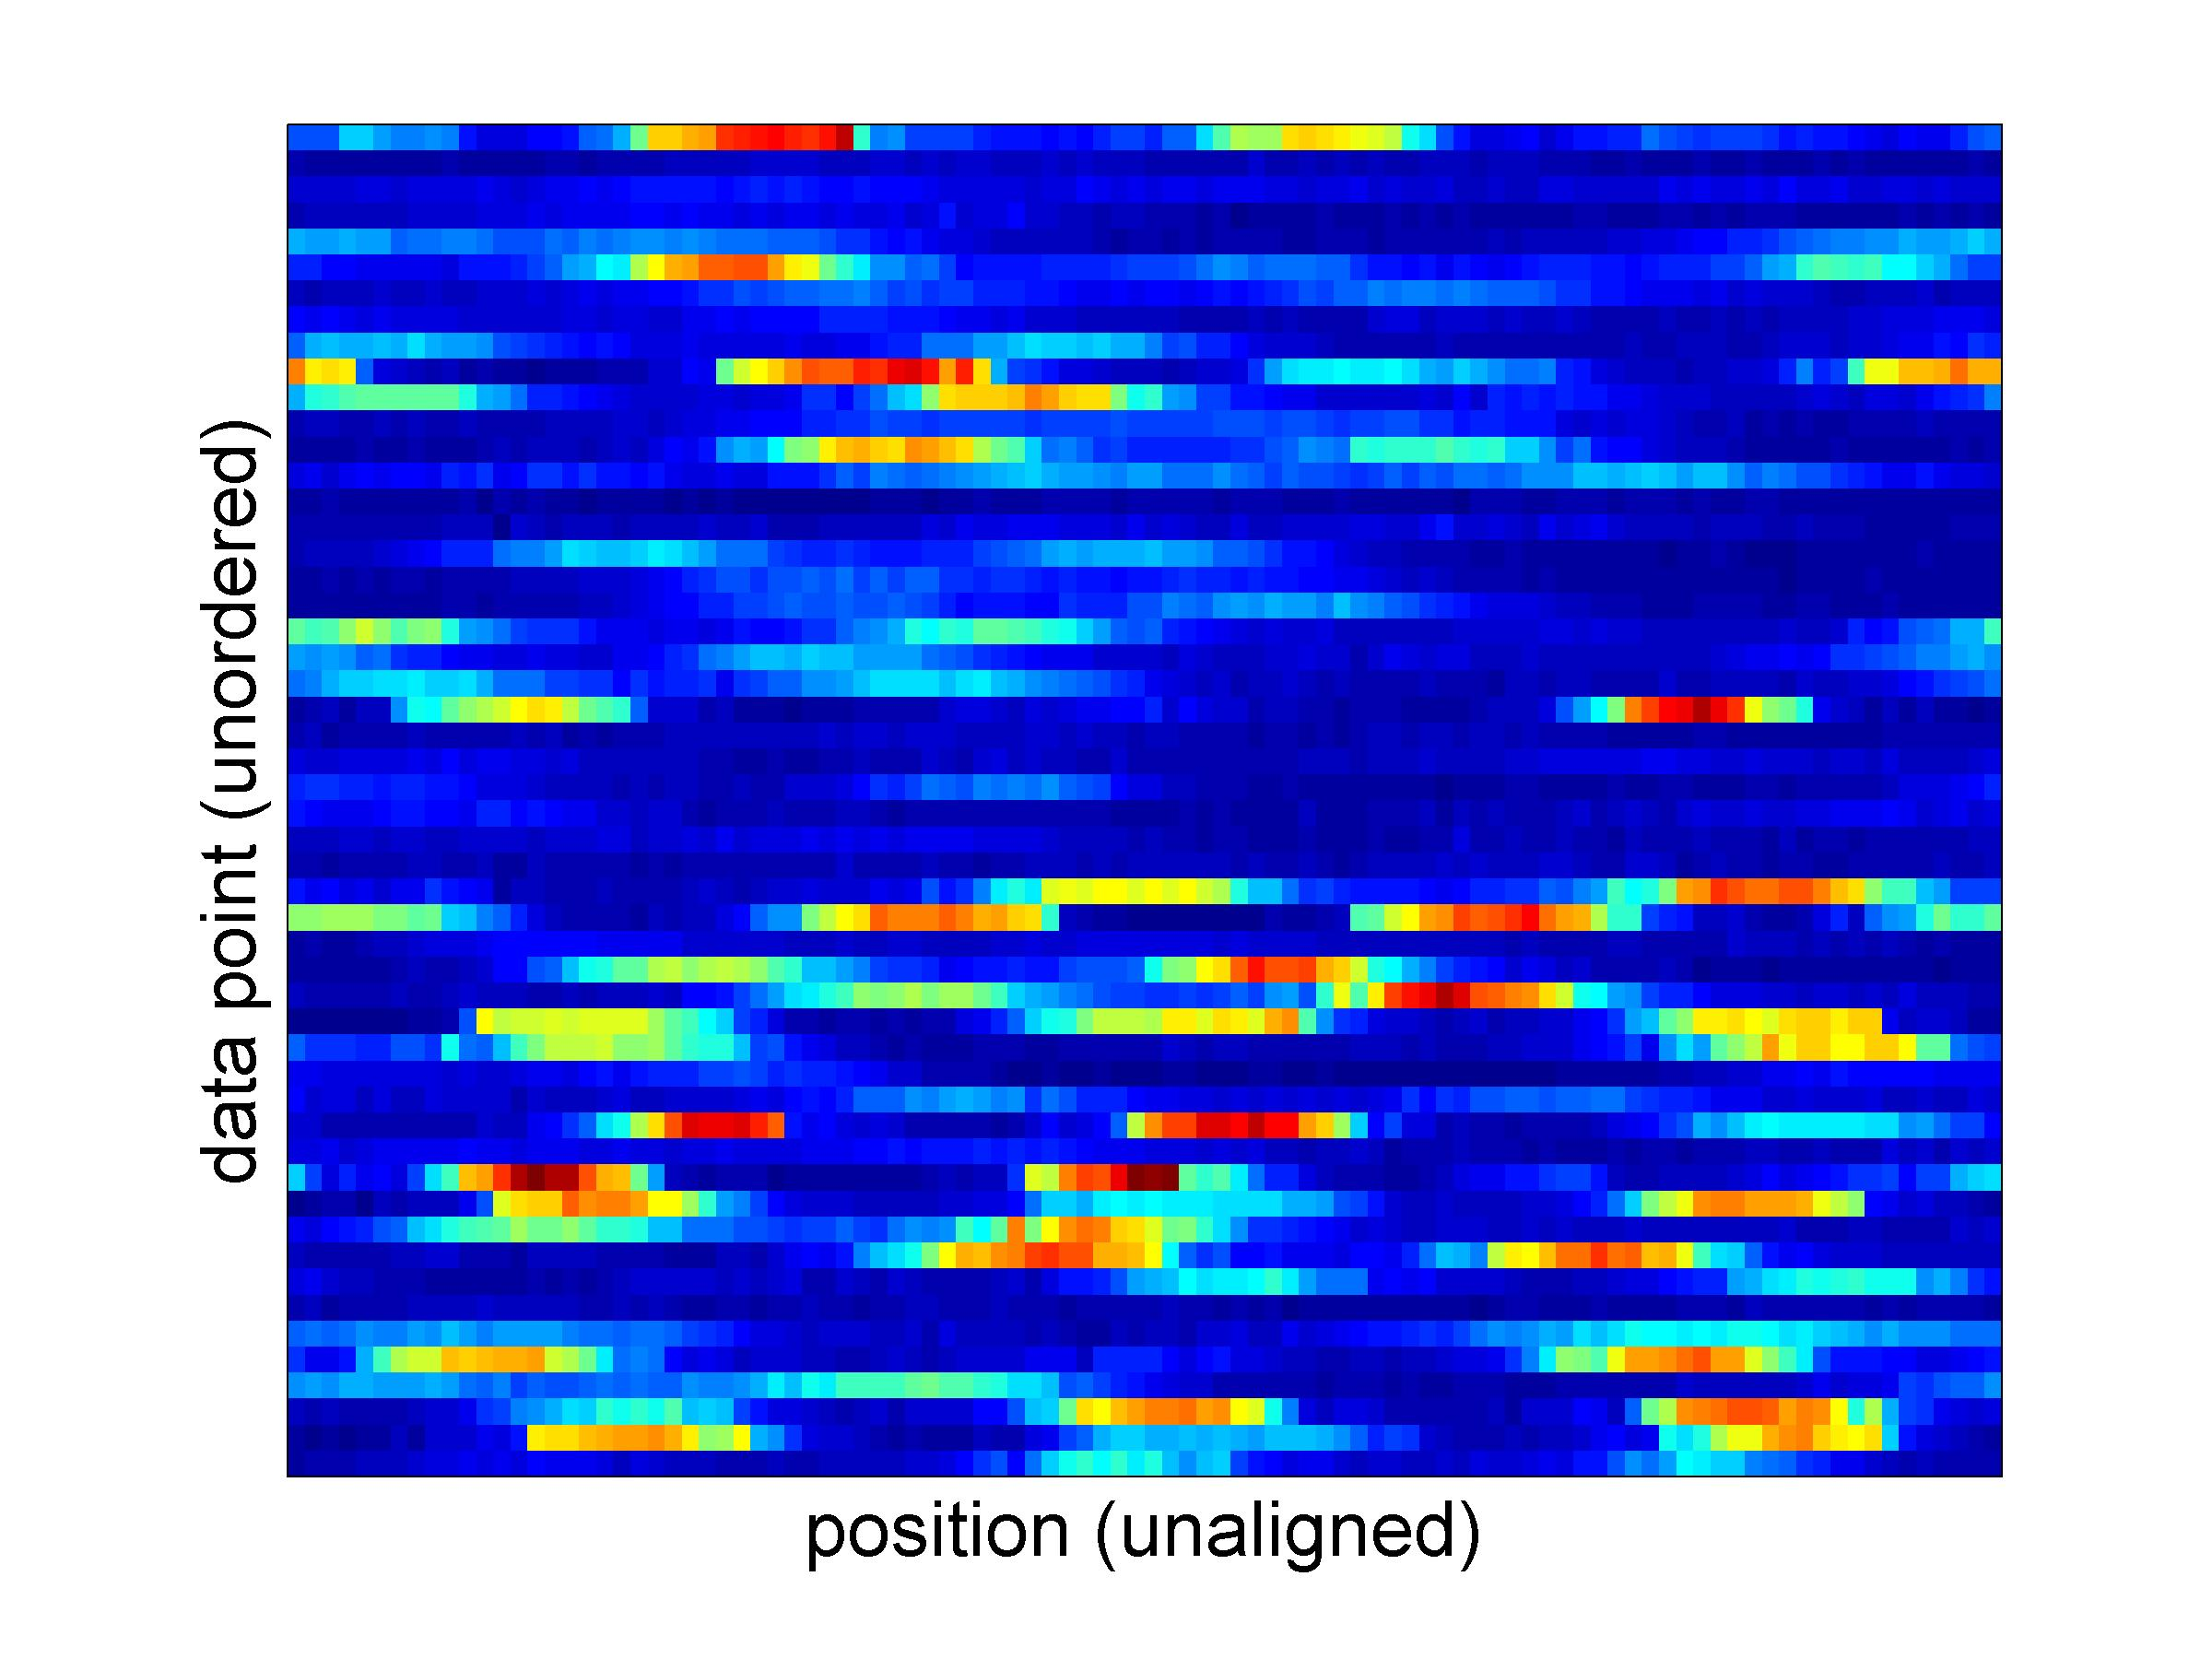
\includegraphics[width=0.35\textwidth]{data_unaligned_unordered}};
		\node[right of=fig1, node distance=0.6\textwidth] (fig2) {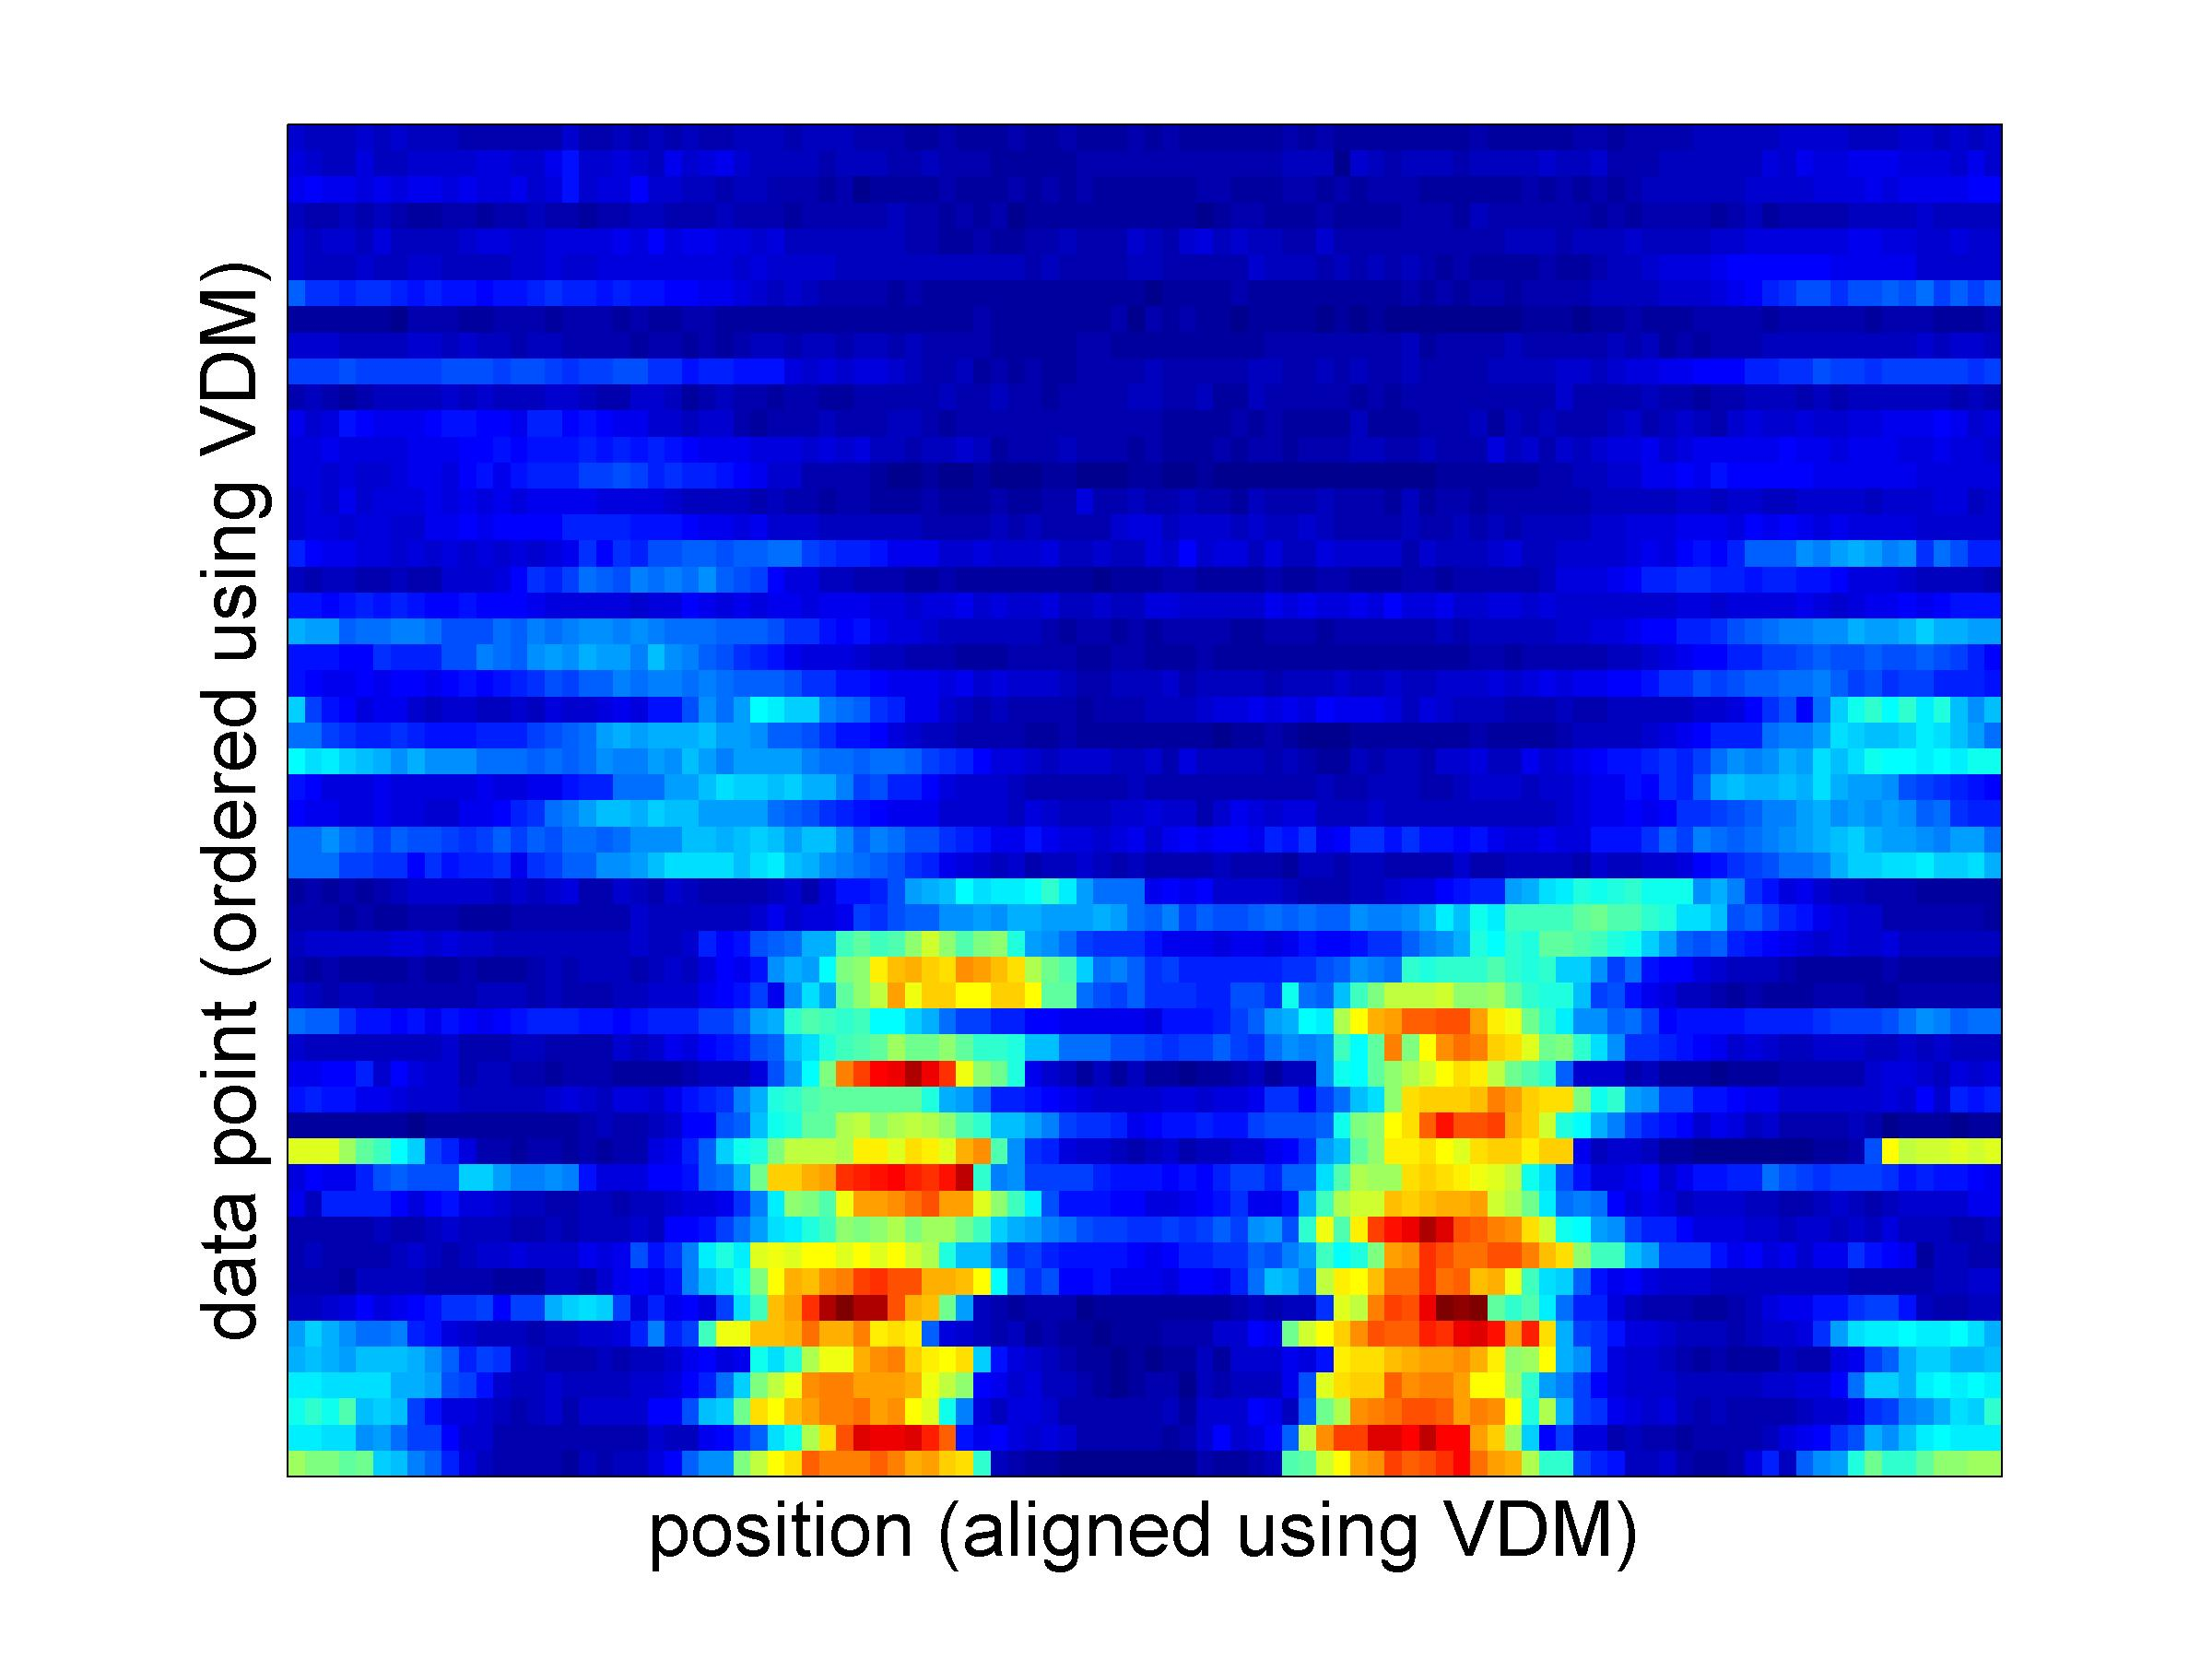
\includegraphics[width=0.35\textwidth]{data_ordered_vdm}};
		\draw[->] (fig1.east) -- (fig2.west) node[above,midway, text width=0.3\textwidth, align=center] { Aligned and ordered using VDM};
		\node[below of=fig1, node distance=0.7in, text width=0.4\textwidth]{{\small Profiles are unaligned and unordered \par}};
		\node[below of=fig2, node distance=0.7in, text width=0.4\textwidth]{{\small Profiles are aligned and ordered using vector diffusion maps} \par };
	\end{tikzpicture}
	
	\begin{minipage}{0.4\textwidth}
	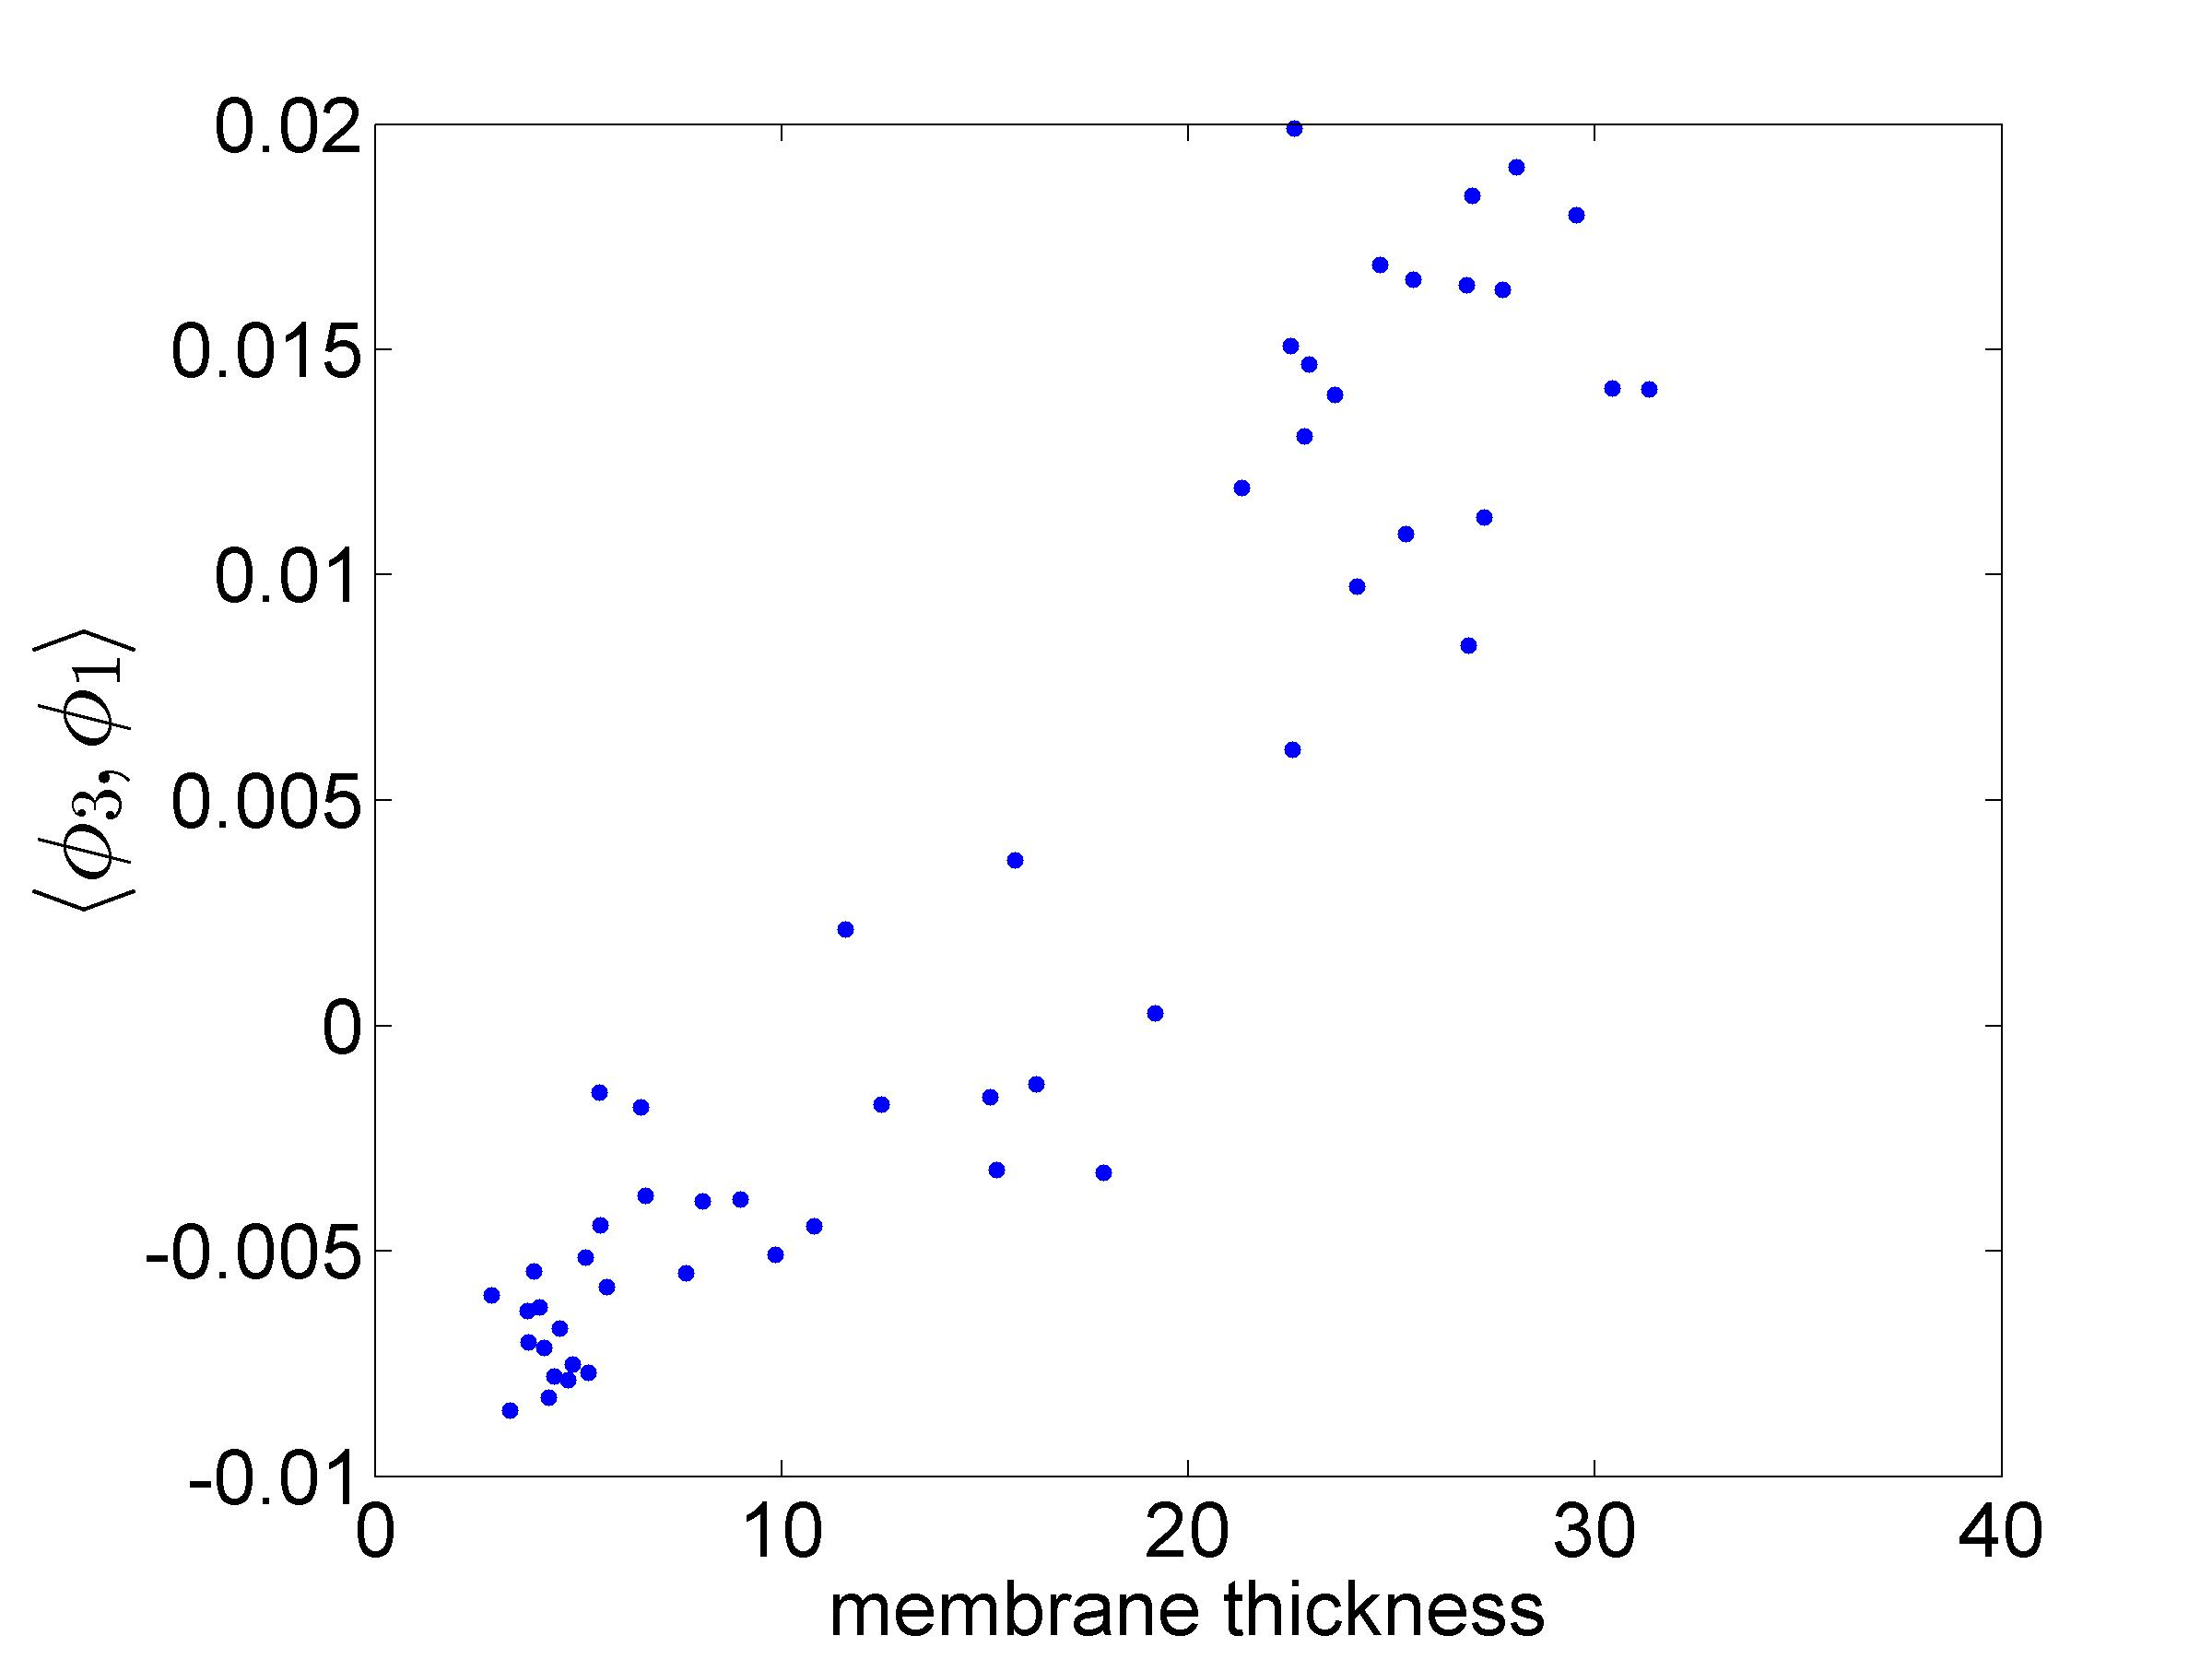
\includegraphics[width=0.9\textwidth]{VDM_time_corr}	
	\end{minipage}
	\begin{minipage}{0.5\textwidth}
	The VDM embedding coordinate, which we use to ``automatically'' order our data, is well-correlated with the membrane thickness, which is known to be monotonic in time.
	\end{minipage}

\end{frame}